%#BIBTEX pbibtex Kitaev_kxy
%!TEX encoding = UTF-8 Unicode
%\documentclass[reprint,amsmath,amssymb,aps,prx]{revtex4-2}
\documentclass[twocolumn,superscriptaddress,showpacs, longbibliography, aps, prb]{revtex4-2}
\usepackage[dvipdfmx]{graphicx}
\usepackage[dvipdfmx]{hyperref}
\usepackage{dcolumn}
\usepackage{physics}
\usepackage{bm}
\usepackage{amsmath,amssymb}
\usepackage{mathtools}
\usepackage{xcolor}
% for Japanese scharacters
%\usepackage[whole]{bxcjkjatype}
\usepackage{hyperref}
\hypersetup{colorlinks=true,breaklinks,linkcolor=blue,urlcolor=blue,citecolor=blue}
\def\vec#1{\boldsymbol #1}
\newcommand{\red}[1]{\textcolor{red}{#1}}
\newcommand{\blue}[1]{\textcolor{blue}{#1}}
\newcommand{\magenta}[1]{\textcolor{magenta}{#1}}
\newcommand{\orange}[1]{\textcolor{orange}{#1}}

\begin{document}


\title{Thermal Hall transport in extended Kitaev models}
\author{Tsuyoshi Okubo}
\affiliation{Institute for Physics of Intelligence, University of Tokyo, Tokyo, 113-0033, Japan}
%\affiliation{JST, PRESTO, Saitama, 332-0012, Japan}
\author{Joji Nasu}
\affiliation{Department of Physics, Tohoku University, Sendai 980-8578, Japan}
% \affiliation{JST, PRESTO, Saitama, 332-0012, Japan}
\author{Takahiro Misawa}
\affiliation{Beijing Academy of Quantum Information Sciences, Haidian District, Beijing 100193, China}
\affiliation{Institute for Solid State Physics, University of Tokyo, 5-1-5 Kashiwanoha, Kashiwa, Chiba 277-8581, Japan}
\author{Yukitoshi Motome}
\affiliation{Department of Applied Physics, University of Tokyo, Tokyo, 113-8656, Japan}

%}

\begin{abstract}
The thermal Hall conductivity---a thermal current analog of the Hall conductivity for electric current---is a useful detector for exotic quasiparticles, %particles,
 such a\red{s %the 
M}ajorana %particles.
fermions, which emerge from quantum many-body effects.
For example, the half-integer quantization of the thermal Hall conductivity at the zero temperature limit
has been regarded as direct evidence of the Majorana %particles. 
fermions.
However, it %has not been clarified 
remains unclear how the thermal Hall conductivity behaves at finite temperatures\red{,} even %for 
in the celebrated Kitaev model on a honeycomb lattice, which is one of the %basic 
\red{fundamental} models for realizing the Majorana %particles 
fermions in quantum magnets\red{, despite the crucial importance to interprete the experimental observations}.  
Here, 
%using a state-of-the-art 
using a finite-temperature tensor network method \red{benchmerked by a thermal pure quantum state technique}, we investigate 
%how the thermal Hall conductivity behaves 
%\orange{behavior of the  thermal Hall conductivity} 
the nature of the thermal Hall conductivity in the Kitaev model with additional interactions under a magnetic field.
We find that the thermal Hall conductivity \red{divided by temperature} significantly %exceeds 
\red{overshoots} the value of the half-integer quantization %in the intermediate temperature range
\red{exhibits a hump while decreasing temperature}, which is consistent with
the experimental results %of 
on \red{a candidate material} $\alpha$-RuCl$_{3}$. 
We also find that the field-\red{direction} %angle 
dependence of the thermal Hall conductivity is
consistent with the sign of the Chern number %of the 
associated with the Majorana fermions,
indicating its topological origin.
We demonstrate that the additional off-diagonal interactions\red{, known as the} %(namely, 
$\Gamma$ and $\Gamma^{\prime}$ terms\red{,} %) %largely 
significantly affect the thermal Hall conductivity. In particular, we show that %negative $\Gamma^{\prime}$ and positive $\Gamma$ 
\red{positive $\Gamma$ and negative $\Gamma^{\prime}$} %terms %remarkably enhance the amplitude 
lead to a remarkable enhancement of the thermal Hall conductivity %at 
in the intermediate temperature region. %We also analyze a classical limit of the extended Kitaev model, %that ignores 
%that does not include quantum effects, as a classical counterpart of quantum systems. 
From the comparison %between 
\red{with} the classical %systems and the quantum systems
\red{counterpart}, we %find 
\red{show} that the effects of the %$\Gamma^{\prime}$ 
\red{$\Gamma$} term %can be captured by the classical model 
\red{go beyond the classical picture, indicating significant quantum fluctuation effects,} while %the effects 
\red{those} of the $\Gamma\red{^\prime}$ term %cannot
\red{is well captured at the classical level.} 
%This indicates that 
%the quantum effects of the $\Gamma$ term are significant. 
%the $\Gamma$ term introduces significant quantum effects.
%Our comprehensive analysis of the thermal Hall conductivity in the extended Kitaev model provides a firm basis for understanding the half-integer quantization of the thermal Hall conductivity in %the Kitaev materials such as $\alpha$-RuCl$_3$.
Our findings establish a comprehensive theoretical framework for understanding 
the thermal Hall %conductivity 
\red{transport} in Kitaev materials such as $\alpha$-RuCl$_{3}$ and 
provide key insights for detecting %and controlling 
the Majorana fermions in quantum spin liquids.
%\red{detectingは良いとして、controlingはこの論文の範囲で何か言えてることがあるのか、不安に思いました。}}
Our developed method also bridges the gap between the theoretical predictions and experimental observations of the thermal Hall conductivity, providing a theoretical foundation for understanding its behavior in a wide range of strongly correlated materials.
\end{abstract}

\maketitle
\section{Introduction}
%Quantum Spin Liquid (QSL) is a highly correlated state of quantum spins 
%without having any long-range orders. 
%Among a variety of QSLs, Kitaev \orange{quantum} spin liquid (KSL) 
%realized as the ground state of the honeycomb lattice Kitaev model~\cite{Kitaev2006} 
%is one of the most studied QSLs in two-dimensional spin models  
%by both experiments and theories~(for a review, see Ref.[\onlinecite{Motome_JPSJ2020}]). 
%Kitaev spin liquid is a キタエフスピン液体は大事。興味をもたれているというこをを書いた方がよい。保留。

\red{[we may break down the following paragraph into a general introduction of fractionalization, quantum spin liquid, and Kitaev QSL; see for instance Kato-san's paper on spin Seebeck]}
Quantum spin liquids (QSLs) are enigmatic states of quantum spin \red{system}s,
which do not %show 
exhibit any 
spontaneous
symmetry breaking even at zero temperature.
Since the QSLs are the source of exotic emergent particles,
such as Majorana %particles (
\red{fermions and} anyon\red{s%)
,} the search for QSLs has been 
one of the central issues of modern condensed matter physics.
Among %several 
various types of QSLs, the Kitaev QSL~\cite{Kitaev2006}, which appears as the ground state
of the Kitaev model on a %the
honeycomb lattice, 
has attracted %a great deal of attention 
significant interest 
%because
sinc\red{e %it has been rigorously 
%shown that 
i}ts low-energy excitations can be \red{rigorously} described by
noninteracting Majorana fermions.
%\blue{noninteracting} Majorana particles appear in low-energy degrees of freedom.
However, it %has been a challenging problem how
remains a challenge to detect the Majorana fermions
in \red{candidate materials for} the Kitaev QSL, since the Majorana fermions are charge-neutral and do not show any characteristic behaviors 
%as a 
in response to electric or magnetic fields.

The thermal Hall conductivity is a promising observable for detecting the
emergent Majorana fermions as they carry heat~\cite{Kitaev2006}.
In the Kitaev model, perturbatively-introduced magnetic fields make the Majorana fermion %systems (systemsはいらない?)
\red{bands} topologically nontrivial.
Accordingly, a
chiral edge current appears, which is protected by %the 
\red{the band topology characterized with} a nonzero Chern number \red{$\nu$}.
Because the chiral edge current is an energy current of Majorana fermions, 
the thermal Hall conductivity %takes 
\red{$\kappa_{xy}$ divided by temperature $T$ is quantized as} %exhibits the half-quantized value 
\begin{align}
{\frac{\kappa_{xy}}{T} = \frac{1}{2} \frac{\pi k_{\mathrm{B}}^2}{6\hbar}}\red{\nu,}
\label{eq:k_xy}
\end{align}
in the zero temperature limit\red{, where $k_{\mathrm{B}}$ and $\hbar$ denote the Boltamann and Dirac constants, respectively}.
\red{Here, $\nu$ takes $\pm 1$ depending on the direction of the magnetic field. This quantized value is half of that for electrons with the same band topology, and hence, it is called the half-integer quantization.} 
%This half-quantization 
\red{Detecting this peculiar behavior} offers
direct evidence of the 
Majorana fermions.

%The thermal Hall conductivity is one of the characteristic phenomena observed 
%in the \orange{KSL} under applied magnetic field~\cite{Kitaev2006}. 
%Based on the Majorana fermions picture, the external magnetic field opens a gap in the bands of %mobile 
%\orange{itinerant} Majorana fermions, 
%and the chiral edge current appears. 
%Due to the chiral edge current, the thermal Hall transport is induced. 
%Because the chiral edge current is a current of \orange{Majorana} fermions, 
%the thermal Hall conductivity takes the half-quantized value 
%\begin{align}
%\orange{\frac{\kappa_{xy}}{T} = \frac{1}{2} \frac{\pi k_{\mathrm{B}}^2}{6\hbar}}
%\end{align}
%in the zero temperature limit.

%Recently, a thermal Hall experiment for $\alpha$-$\mathrm{RuCl_3}$ 
%reported that the half-quantization of the thermal Hall conductivity occurs
%under a tilted magnetic field~\cite{Kasahara_Nature2018}.
%Recently
\red{Strikingly}, \red{such a half-integer quantization was reported in the} %a 
thermal Hall experiment for \red{a quasi-two-dimensional van der Waals magnet} $\alpha$-$\mathrm{RuCl_3}$ 
%has reported the observation of half-\red{integer} quantization 
\red{u}nder \red{a %tilted 
m}agnetic field~\cite{Kasahara_Nature2018}.
Although $\alpha$-$\mathrm{RuCl_3}$ shows magnetic zigzag order at zero magnetic field~{\cite{Sears_PRB2015,Williams_PRB2015,Cao_PRB2016}}, 
inelastic neutron scattering measurements %suggested 
suggest that applying \red{a} magnetic fiel\red{d} %s induces 
drives the syste\red{m} %s 
into
%the Kitaev 
\red{a} QSL~\cite{Banerjee_npjQ2018}.
Th\red{e %observed 
h}alf-\red{integer} quantiz\red{ation observed in this field regime} %ed thermal Hall conductivity 
%indicates 
\red{suggests} that topologically\red{-}nontrivial Majorana bands %emerge 
\red{are realized} in th\red{is material. %e Kitaev candidate material
%$\alpha$-$\mathrm{RuCl_3}$ under magnetic fields. 
%A s
S}imilar %half-quantized thermal Hall conductivity 
%were 
\red{quantization was} observed %under 
\red{even when subjected to an} in-plane magnetic fiel\red{d, %s 
in contrast to the conventional thermal Hall effect of electrons that requires an out-of-plane field~\cite{Yamashita_PRB2020,Bruin_NPhys2022}}.
It %h
\red{w}as also shown that %the angular 
%magnetic-
\red{f}ield angle dependence of the thermal Hall conductivit\red{y
%on the magnetic field 
i}s consistent with %those 
that in the Kitaev model\red{, suggesting that the Majorana fermion bands in the real material have the same topology predicted by the Kitaev model}~\cite{Yokoi_Science2021}\red{.}
%An independent measurement of the thermal Hall conductivity has also %shows 
%reported the half-integer quantization of the thermal Hall conductivity
%~\cite{Bruin_NPhys2022}.

However, there remains controversy on interpreting the observed thermal Hall transport as %the 
evidence of the Kitaev QSL. 
For example, the observed thermal Hall conductivity %shows 
\red{exhibits} an overshoot\red{ing behavior while decreasing temperature before converging to} %of 
%beyond 
the half-\red{integer} quantized value\red{.} 
%for higher temperatures, 
%and t
\red{T}he origin of %such overshooting 
\red{this} behavior %has not been 
\red{remains un}resolved\red{,}  %while 
although contributions from phonons~\cite{Ye2018Quantization,Vinkler2018} and visons~\cite{Joy2022} %have been 
\red{were} proposed. 
In addition, real compounds, including $\alpha$-$\mathrm{RuCl_3}$, %could 
\red{may} contain additional interactions \red{not included in the Kitaev model,} 
such as the Heisenberg interactio\red{n}%s
~\cite{Chaloupka_PRL2010,Chaloupka_PRL2013}, and the \red{symmetric} off-diagonal $\Gamma$ and $\Gamma'$ interactions~\cite{Rau2014,Rau2014pre,Winter2016}\red{, whose} %. 
%The 
effect\red{s remain elusive.} %of such additional interactions on the thermal Hall conductivity 
%beyond the perturbation theories~\cite{TakikawaF2020, YamadaF2021}, %is
%has not yet been fully clarified. %yet.

Furthermore, several %later 
\red{subsequent} experiments %for 
on $\alpha$-$\mathrm{RuCl_3}$ %discussed relationship 
\red{have reported the absence of half-integer quantization.} 
%to 
\red{For instance, instead of the quantization in the transverse component, %with 
quantum oscillations \red{were} observed in the longitudinal thermal conductivity~\cite{Czajka_NPhy2021}\red{. Additionally}, 
other origins of the thermal Hall response were discussed, e.g.,} topological magnons~\red{\cite{Czajka_NMat2023,McClartyDGRPMP2018,Joshi2018}}, 
 para-magnon~\cite{Hentrich_PRB2019}, \red{and}
 phonons~\cite{Lefra_PRX2022}\red{. 
%However, the origin of the thermal Hall conductivity has not been settled. 
T}o resolve the origin of the thermal Hall conductivity observed in experiments, 
it is %demanding 
crucial to \red{obtain reliable results by} perform\red{ing} unbiased analysis  
of the thermal Hall conductivity in the Kitaev model and its extensions\red{.} %, without 
%assuming any quasiparticle excitations.

%Although t
\red{T}he thermal Hall transport in the pure Kitaev model has been well-understood 
in the limit of zero temperature 
and weak magnetic fields \red{as mentioned above~\cite{Kitaev2006}.} %, which %are introduced 
%can be treated by perturbation expansions
%~\cite{Kitaev2006}, 
%the 
%accurate analysis of the thermal Hall conductivity under
%magnetic fields beyond the perturbation theory is limited. 
For finite-temperature properties, %we may use 
%Monte Carlo 
\red{while several numerical} simulation \red{methods %for 
have been developed, they are applicable only} 
at zero magnetic field\red{, %s
where the thermal Hall response vanishes, because of a negative sign problem~\cite{NasuUM2014,NasuUM2015,YoshitakeNM2016,YoshitakeNKM2017,YoshitakeNM2017, YoshitakeNKM2020}}. 
%These calculations successfully showed a double-peak structure in the specific heat and its relationship %to 
%with the Majorana fermions. 
%Unfortunately, 
%However, in order to treat finite 
%magnetic fields, 
%which is necessary for thermal Hall transport, we need to consider an effective interaction %justified only for 
%that is valid only at sufficiently small magnetic fields to avoid the negative sign problems~\cite{NasuYM2017}. 
%Numerical simulations based on the 
\red{A quantum Monte Carlo simulation based on a Majorana fermion representation has been performed for an} effective model \red{derived by a perturbation expansion with respect to the magnetic field~\cite{NasuYM2017}. 
It} showed a non-monotonic temperature dependence 
%of 
in the thermal Hall conductivity %: it has 
\red{with} a weak peak at high temperature\red{, %and 
%converges to the half-quantized value~\cite{NasuYM2017}. 
%However, 
but the result cannot explain the overshooting behavior observed in experiments since} the peak value is much smaller than the half-\red{integer} quantized value\red{.} %, 
%and then, 
%the %huge 
%large $\kappa_{xy}$ beyond the half-quantized value, 
%which is observed in the experiment %of 
%on $\alpha$-$\mathrm{RuCl_3}$, 
%has not been explained by the effective model based on the perturbation theory.
% \blue{\cite{Rau2014,Rau2014pre}はどこかで引用}

The effects of %the symmetric off-diagonal 
\red{non-Kitaev} interaction\red{s %called $\Gamma$ and $\Gamma'$ terms, 
h}ave also been investigated based o\red{n %the 
p}erturbative %treatment
\red{arguments.} %justified in the %situation 
%regime of small magnetic fields 
%and small off-diagonal interactions~\cite{TakikawaF2020, YamadaF2021}. 
\red{For instance,} %In the case of the $\Gamma'$ interaction, 
it was shown that the $\Gamma'$ term introduces 
an additional contribution to the gap of Majorana fermion band~\cite{TakikawaF2020}\red{; %.
%\textcolor{red}{(Is it better to explicitly write down the relationship 
%between the gap and parameters? If so, we may need to define the Hamiltonian before this paragraph.)}  Maybe not necessary
%T
t}h\red{e %total 
g}ap %is increased (decreased)
increases (decreases)
%for 
with a negative (positive) $\Gamma'$ interaction\red{, which might affect} %.
%Thus, 
the finite-temperature behavior of the thermal Hall conductivity\red{.} %might largely depend on the sign of $\Gamma'$. 
%Based on %the similar perturbation theory, 
%a similar perturbation approach, Ref.~\cite{YamadaF2021} %discussed 
%showed that 
\red{In contrast,} the 
effect of the $\Gamma$ interaction %appeared 
appears %as the third-order contribution. 
\red{at a higher-order expansion~\cite{YamadaF2021},}
%Although %it indicates 
%this 
suggest\red{ing} %s 
\red{weaker influence on} %that the effect of $\Gamma$ in 
the thermal Hall transpor\red{t %is %less 
%weaker 
t}han that of $\Gamma'$\red{. %, 
%t
T}he same analysis also showe\red{d %a possible 
q}uantum phase transition\red{s, %induced by the effective interaction arising from %the 
%third-order perturbation. 
which may lead to} 
%Therefore, a 
no\red{n%-
t}rivial effect\red{s.} %may be induced by %the 
%such phase transitions.
\red{[refer to PRL 122, 147203 (2019)?]} 
%Note that, as we mentioned, 
\red{Nonetheless, all} these analyses are based on %the
perturbation theory justified for small $\Gamma$ and \red{$\Gamma'$ %. 
%Furthermore, the connections to the thermal Hall transport 
%are only
%have only been discussed %within 
i}n the zer\red{o %-
t}emperature limit. 
\red{Recently, an unbiased calculation using a tensor network method was conducted for the thermal Hall conductivity in the Kitaev-Heisenberg model~\cite{KumarT2023}, but the definition of energy current remains incomplete, as detailed later.} 
Thus, %to 
\red{for a comprehensive} understand\red{ing of} the effect\red{s} of the %off-diagonal 
\red{non-Kitaev} interactions %at finite temperatures
\red{on the thermal Hall transport}, it is necessary to %perform an analysis 
\red{explore a theoretical framework with proper definition of energy current,} beyond %the 
perturbation theory.

\if0{
%As the 
One possible origin of the thermal Hall transport at finite temperatures %, we can also consider 
is topological magnons, which are excited from the magnetic order induced by %the 
applied magnetic fields \cite{McClartyDGRPMP2018,Joshi2018}. 
The edge modes due to such topological magnons %exist 
have
 %with 
a nonzero gap, %at high energies, 
%and then the corresponding 
so that the
thermal Hall transport %becomes zero 
vanishes in the zero temperature limit. 
However, at finite temperatures, we need to consider %a 
contributions from such topological 
magnons in addition to the contributions from the Majorana fermions. 
In realistic situations, the thermal Hall transport might not be 
explained solely by either the Majorana fermions or bosonic quasiparticles such as topological magnons and phonons.
%[一応phononも追加してみましたが不要なときは削除ください]}
% or the topological magnons. 
To understand the thermal Hall transport at %a 
finite temperatures, 
%we need %to treat 
an unbiased %method that can treat
approach is required to handle the complex interplay of
these contributions.
%a complicated mixture of these contributions. 
}\fi

In this paper, we investigate the thermal Hall transport in 
%the 
\red{an} extended Kitaev mode\red{l%s
,} which include\red{s} the \red{symmetric} off-diagonal interactions, \red{$\Gamma$ and $\Gamma^\prime$,} 
%by 
using a finite-temperature tensor network method %and %the 
%an approach exploiting the 
\red{benchmarked with a}
thermal pure quantum state %s
\red{method}. 
For comparison, we also perform %the 
classical Monte Carlo simulations
%for 
in the classical limit of %the 
%extended Kitaev 
\red{the} mode\red{l%s
.}
We properly define the energy current from the model Hamiltonian 
and calculate the edge current in the systems with open boundaries. 
This treatment does not assume %any origins 
a specific origin for %of 
the thermal Hall transport, 
and %considers 
\red{includes} all contributions on an equal footing.  
We find that %this 
the calculated thermal Hall conductivity shows a clear overshooting behavior similar to the experimental observations, %indicating 
\red{suggesting} that the experimentally\red{-}observed thermal Hall conductivity %might 
\red{can} be \red{qualitatively} explained by %the 
%simple 
\red{the} extended Kitaev mode\red{l%s
.}
%We also %discuss 
%analyze 
\red{Through comprehensive analyses of} the effect\red{s} of %off-diagonal interactions on the thermal Hall conductivity. 
\red{$\Gamma$ and $\Gamma^\prime$,} 
%Indeed, 
we %find 
\red{demonstrate} that depending on the sign and %the 
type of %the 
%off-diagonal %couplings,
\red{these} interactions, the thermal Hall conductivity can %change 
\red{vary in both magnitude and} %its 
sign at finite temperatures. 
\red{In particular, we find that the thermal Hall conductivity is significantly enhanced by positive $\Gamma$ and negative $\Gamma^\prime$ in an intermediate temperature range.} 

The organization of this paper is as follows. 
In Sec.~\ref{sec:model}, we introduce the extended Kitaev model and
give a brief overview of previous studies on %the extended Kitaev model.
this model.
In Sec.~\ref{sec:method}, we explain %how to calculate the
the procedure for calculating the
thermal Hall conductivity %for 
in the extended Kitaev model.
We also %explain 
\red{introduce} the \red{numerical} methods used in this study, i.e.,
the exponential tensor renormalization (XTRG) method,
the \red{canonical} thermal pure quantum state (\red{c}TPQ) method, and
%the 
classical Monte Carlo simulations.
In Sec.~\ref{sec:pureKitaev}, we show the temperature
dependence of the thermal Hall conductivity for the pure Kitaev model under a magnetic field
along the [111] direction. We also show the field-\red{direction} %angle 
dependence 
of the thermal Hall conductivity.
In Sec.~\ref{sec:Gamma}, we show how the off-diagonal interactions
$\Gamma$ and $\Gamma^{\prime}$ %terms 
affect the temperature
dependence of the thermal Hall conductivity.
In Sec.~\ref{sec:classicalMC}, we analyze 
the thermal Hall conductivity in the classical limit of the Kitaev model.
Section~\ref{sec:Summary} is devoted to a summary and discussion.


\section{Model}
\label{sec:model}
To investigate the thermal Hall conductivity %transport 
in \red{the} Kitaev \red{spin} systems, 
we consider an extended Kitaev model containing the \red{symmetric} off-diagonal $\Gamma$ and $\Gamma'$ interactions 
%together with the Kitaev interaction 
on the honeycomb lattic\red{e.} %(Fig.~\ref{fig:lattice}). 
The Hamiltonia\red{n %of the model under a magnetic field 
i}s given %as
by
\begin{equation}
 \mathcal{H} = \sum_{\gamma = x,y,z} \sum_{\langle i,j \rangle_\gamma}\mathcal{H}_{ij}^\gamma -  \sum_{i,\gamma} h^\gamma S_i^\gamma,
 \label{eq:model-Hamiltonian}
\end{equation}
with
\begin{align}
 \mathcal{H}_{ij}^\gamma &= \Bigl[ K S_i^\gamma S_j^\gamma + \Gamma\left( S_i^\mu S_j^\nu + S_i^\nu S_j^\mu \right) \notag\\
&\qquad + \Gamma'\left( S_i^\mu S_j^\gamma + S_i^\nu S_j^\gamma + S_i^\gamma S_j^\mu + S_i^\gamma S_j^\nu \right) \Bigr]\\
&= \sum_{\alpha,\beta = x,y,z} J_{\alpha\beta}^\gamma S_i^\alpha S_j^\beta, 
\end{align}
where $\langle i,j\rangle_\gamma$ %means 
denote\red{s %the 
n}earest\red{-}neighbor pair\red{s} o\red{n %the 
$\gamma$}-bond\red{s on the honeycomb lattice [see Fig.~\ref{fig:lattice}(a)], and $S_i^\gamma$ represents the $\gamma$ component of the spin-$1/2$ operator at site $i$;} %. 
$(\mu, \nu, \gamma)$ %represents 
is a cyclic permutation of $(x,y,z)$, for example,
$(\mu, \nu, \gamma)=(y,z,x)$ for the $x$-bond.
\red{The second term in Eq.~\eqref{eq:model-Hamiltonian} represents the Zeeman coupling to an external magnetic field $\bm{h} = (h^x, h^y, h^z)$.}
% Throughout the paper, we consider the ferromagnetic Kitaev interaction $K= -1$. 
% \red{We also set the amplitude of the primitive translation vector of the honeycomb 
% lattice to the unit length and \orange{$k_B = \hbar = 1$.}} We discuss, typically, physical quantities 
% for the model on \red{$(L, L') = (6, 6)$} shown in Fig.~\ref{fig:lattice}(a). \orange{The total system size is given by $N_{\rm s}=2\times L\times L^{\prime}$.} 
% In Appendix \ref{app:XTRG_Bench}, we compare the results with those of \red{$(L, L') = (4, 8)$}. 

% \blue{XC4、XC6という表現が少しマニアックな気がします。$(L,L')=(4,6),(6,6)$とかの方がわかりやすい?
% もしくは、$L_X=2L$、$L_Y=L'/2$のように基本並進ベクトル基準にして、実空間を$\bm{R}=(X,Y)$で表現した方がよいかもしれないです。
% この場合、site positionも$\bm{R}_i$として、$\kappa_{XY}$のように表現すべきかもしれません。}\red{$(L,L')$方式を採用してみる。}

\begin{figure}
  \begin{center}
    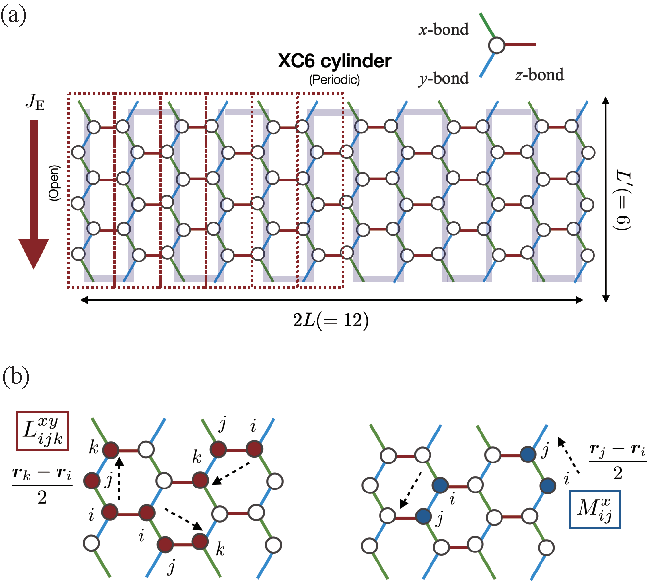
\includegraphics[width=\linewidth]{Figs/lattice.pdf}
  \end{center}
  \caption{(a) Schematic view of %an $(L, L') = (6, 6) $ 
\red{the} honeycomb lattice structure \red{with  $(L, L') = (6, 6) $,} consisting of 72 sites\red{, which is typically used in the XTRG calculations}. 
\red{The inset represents $\gamma$-bonds in the Hamiltonian in Eq.~\eqref{eq:model-Hamiltonian}.} 
%Along the vertical direction, w
\red{W}e impose the periodic \red{and open} boundary conditions \red{along the vertical and horizontal directions, respectively.} %, 
%  while %the left and the right boundaries are open. 
%  the open boundary condition is imposed in the horizontal axis. %}
  We consider the thermal current $J_{\mathrm{E}}$ in a downward direction indicated by the arrow. In the tensor network simulation, we consider a snake-like matrix product operators indicated by the gray thick line behind the lattice. (b) Graphical representations of the three-body ($\red{L_{ijk}^{\gamma\gamma^\prime}}$) and the two-body ($\red{M_{ij}^\gamma}$) terms in the definition of the thermal current \red{in Eq.~}\eqref{eq:def_J}.
\red{[omit ``XC6 cylinder" in (a)?]} 
\red{[indicate ``$l=1$", `$`l=2$", ... above or below the dotted boxes in (a)?]} 
\red{[place the boxes in (b) above each panel?]} 
}
  \label{fig:lattice}
\end{figure}

%\red{To investigate the magnetic property of the model, we defined the magnetization parallel to the appliged magnetic field, $M_{\parallel}$, as $M_\parallel=\vec{M}\cdot\vec{h}/|\vec{h}|$, where $\vec{M} = \frac{1}{N}\sum_i \vec{S}_i$ is the total magnetization.}

%\orange{\bf [ここでもっと詳しく、K-G-G'模型の基底状態の先行研究について触れる必要がある?]}\blue{[$\to$加えてみましたがイントロに持ってきてもよいかもしれません。]}
\red{A microscopic origin of the Kitaev interaction $K$ in Eq.~\eqref{eq:model-Hamiltonian} was proposed for effective $j_{\rm eff}=1/2$ moments in spin-orbit coupled Mott insulating systems~\cite{Jackeli_PRL2009}. 
It was pointed out that magnetic ions with $t_{2g}^5$ electron configurations comprise the spin-orbit entangled $j_{\rm eff}=1/2$ states under the strong spin-orbit coupling, and exchange processes with indirect hoppings via ligands generate the bond-dependent Kitaev-type interactions between the $j_{\rm eff}=1/2$ moments in edge-sharing octahedral coordinates.} 
The \red{symmetric off-diagonal} %symmetric spin 
interaction\red{s %with 
%denoted by 
$\Gamma$} and $\Gamma'$ were %first introduced
%originally proposed in Ref.~\cite{Rau2014} 
\red{introduced} as additional contributions %to the Kitaev and Heisenberg interactions.
\red{arising from different exchange processes~\cite{Rau2014}.} 
%These interactions %are given 
%arise as superexchange-type couplings between nearest neighbor $j_{\rm eff}=1/2$ spins in transition metal ions with strong spin-orbit coupling where neighboring octahedra consisting of ligand ions share their edges.
%They are derived by performing perturbation expansions in the strong correlation limit of the three-orbital Hubbard model for the $t_{2g}^5$ configuration~\cite{Jackeli_PRL2009}.
%The virtual hoppings via $p$ orbitals in ligand ions %mainly dominate 
%primarily govern the exchange process, and direct hoppings between the neighboring $d$ orbitals are secondary.
%The former induces the Kitaev and $\Gamma$ interactions, but the Heisenberg interaction is caused only by the latter. Hence, the Kitaev and $\Gamma$ interactions are %believed to be leading interactions for 
\red{On one hand, the $\Gamma$ interaction is derived by the exchange process including both direct and indirect hoppings, which can be relevant} 
%considered to be the dominant interactions
%governing the magnetic properties 
in Kitaev candidate materials~\cite{Yamaji2014,Winter2016,Winter_2017rev}.
\red{On the other hand, %T
t}he $\Gamma'$ interaction %does not appear %in the case where
\red{is induced by symmetry lowering of} 
%when 
the octahedra surrounding %transition metal 
\red{magnetic} ions %retain 
\red{from} the cubic symmetry\red{, %.
%The symmetry lowering by a trigonal distortion, 
%which is 
i}nevitabl\red{y existing} %e 
in real materials\red{~\cite{Rau2014}.} %, %results in 
%induces this interaction~\cite{Rau2014}.
%The spin excitations and thermodynamic properties of extended Kitaev models, including $\Gamma$ and $\Gamma'$ interactions, have been calculated, and 
\red{The} realistic \red{values of interaction} parameters have been %examined to reveal the magnetic properties of 
\red{extensively discussed for} the Kitaev candidate material\red{s~\cite{Yamaji2016,Suzuki2018,laurell2020dynamical,Maksimov2020}.} %, iridium oxides $A_2$IrO$_3$ ($A=$Na,Li) and $\alpha$-RuCl$_3$~\cite{Yamaji2016,Suzuki2018,laurell2020dynamical,Maksimov2020}.
Most theoretical works have suggested $K<0$ and $\Gamma>0$ for \red{the primary candidate} $\alpha$-RuCl$_3$\red{,} %but 
although the sign of $\Gamma'$ %is still 
remains under debate.

%Because of the complexity of realistic models, t
\red{T}he $K$-$\Gamma$ model\red{, which is given by Eq.~\eqref{eq:model-Hamiltonian} with $\Gamma^\prime=0$,} has been %recently 
\red{intensively} studied %recently 
as a simplified \red{realistic} model\red{, by %.
%This model has been examined %by 
using various theoretical methods, such as} the exact diagonalization~\cite{catuneanu2018,Yamada2020}, \red{the %D
d}ensity %M
\red{m}atrix %R
\red{r}enormalization %G
\red{g}rou\red{p %(DMRG) 
m}ethod~\cite{Gohlke_PRB2018}, 
%tensor network \orange{methods}
\red{the} infinite %P
\red{p}rojected %E
\red{e}ntangled %P
\red{p}air %S
\red{s}tat\red{e %(iPEPS) 
m}ethod~\cite{Lee_NCom2020,ZhangLLLW2023}, a variational approach~\cite{Zhang2021}, \red{the} spin-wave theory~\cite{Smit2020}, and a classical spin approach~\cite{Rayyan2021}.
In the \red{classical limit, %$K$-$\Gamma$ 
this} model %, there is a large 
\red{exhibit macroscopic} degeneracy\red{. %in the classical limit.
%Once q
Q}uantum fluctuations %are taken into account, 
\red{lift this degeneracy, %quantum-disordered states could %potentially 
%emerge, 
b}ut the detailed phase diagram %is still 
remains controversial.
The introduction of the $\Gamma'$ interaction to the $K$-$\Gamma$ model with $K<0$ and $\Gamma>0$ %brings about 
induces \red{magnetically} ordered phases\red{: %in addition to quantum-disordered states.
%It has been pointed out that 
a positive $\Gamma^\prime$ stabilizes} a ferromagnetic phase and \red{a} chiral spin \red{ordered} phase with nonzero spin scalar chiralit\red{y% appear %in the case with
%for $\Gamma'>0$
~\cite{Luo2022PRR,Luo2022}, and} %.
%On the other hand, %the 
a negative $\Gamma'$ induces the zigzag order, which has been observed in Kitae\red{v %-
c}andidate materials at low temperatures~\cite{Rusna2019,gordon2019theory,Chern2020,Lee_NCom2020}. %}
% \orange{
% The ground state phase diagram %of this extended Kitaev model ($K$-$\Gamma$-$\Gamma^{\prime}$ model)
% has been investigated by 
% the DMRG method~\cite{Gohlke_PRB2018} and the tensor-network method~\cite{Lee_NCom2020}. 
% It is shown that the zigzag state is stabilized by small but finite $\Gamma$ and $\Gamma'$.}
Thus, %this 
\red{the $K$-$\Gamma$-$\Gamma^\prime$} model \red{in Eq.~\eqref{eq:model-Hamiltonian}} might be suitable %to investigate 
for investigating the relevant 
effects of \red{symmetric} off-diagonal interactions on the thermal Hall conductivity in real compounds including $\alpha$-$\mathrm{RuCl_3}$.


%Throughout the paper
\red{In the following sections}, we consider the ferromagnetic Kitaev interaction \red{by setting} $K= -1$, which %is naturally expected 
naturally arises from the %super
\red{e}xchange process in \red{the} $t_{2g}^5$ systems\red{~\cite{Jackeli_PRL2009}}. 
\red{For $\Gamma$ and $\Gamma^\prime$, we consider both positive and negative cases.} 
We %also 
\red{take $k_{\rm B} = \hbar = 1$ and} set the %amplitude 
\red{length} of the primitive translation vector of the honeycomb 
lattice to the unit length\red{.} %and $k_B = \hbar = 1$. 
We typically %discuss %, typically, 
\red{compute} physical quantities 
for the model %on 
\red{on a finite-size cluster} with $(L, L') = (6, 6)$ shown in Fig.~\ref{fig:lattice}(a)\red{, including} %. The total system size is %given by 
$N_{\rm s}=2\times L\times L^{\prime} \red{=72}$ \red{spins}.
%In Appendix \ref{app:XTRG_Bench}, 
%\orange{we investigated the bond dimension dependence of physical quantities for system sizes $(L, L') = (6,6)$ and $(4,8)$.}
%\orange{\bf この文はあとでも触れているので不要?}
%we compare the results with those of \red{$(L, L') = (4, 8)$}. 

\section{Method}
\label{sec:method}
In this section, we %\orange{introduce definition}
introduce \red{the methods used in this study. 
First, we define %the definition of 
the energy current and} 
the thermal Hall conductivity %for finite-size clusters described above
\red{in Sec.~\ref{subsec:Thermal Hall conductivity}}. Then, we %explain %three 
describe %three
\red{two} 
numerical methods for calculating the finite-temperature %properties of the model. 
\red{behaviors: a tensor network method called the XTRG method in Sec.~\ref{subsec:Tensor network method} and the cTPQ method in Sec.~\ref{subsec:Thermal pure quantum state}. 
We employ the former for main calculations on the $(L, L') = (6, 6)$ cluster introduced above, and use the latter for the benchmark in smaller size clusters.}
%To investigate quantum spin models, we employ two methods. 
%For smaller clusters, we use the thermal pure quantum state (TPQ) method %,while 
%and we employ a tensor network-based method for larger clusters. 
%As 
\red{Finally, in Sec.~\ref{subsec:Classical Monte Carlo simulation}, we briefly describe the method of classical Monte Carlo simulation to study} a %reference 
classical counterpart to th\red{e %quantum 
m}odel\red{.} %, 
%we investigate the classical spin model with the same interaction coefficients
%by using %the 
%classical Monte Carlo simulations. 

\subsection{Thermal Hall conductivity}\label{subsec:Thermal Hall conductivity}
%{\bf \orange{このkappaxyの定義に関して引用文献は必要?}}\blue{[$\to$追加してみました]}
To investigate the thermal Hall conductivity in %the 
Kitaev systems, w\red{e %first 
d}efine 
%the energy current $\bm{J}_{\mathrm{E}}$ through the commutation relation between the Hamiltonian and 
the energy polarization %$\bm{P}_{\mathrm{E}}$, which %are
%is defined %as
%by
\red{as}~\cite{Katsura2010,NasuYM2017}
%$\bm{P}_{\mathrm{E}}$, as $\bm{J}_{\mathrm{E}} =  i \left[\mathcal{H}, \bm{P}_{\mathrm{E}}\right] \notag$
%\blue{, where the reduced Planck constant is set to be unity [$k_B$を1にすることと長さの単位についても言及した方がよいかもしれません。]}\red{Modelのところの$K=-1$のところに単位などについて、まとめて書くことにした。$\hbar$はとりあえずここのまま。}. 
%$\hbar$はkbのところで1にすると宣言
%The energy polarization is defined as 
\begin{equation}
 \bm{P}_{\mathrm{E}} = \sum_{\alpha,\beta,\gamma}\sum_{\langle i,j\rangle_\gamma} \frac{\bm{r}_i + \bm{r}_j}{2} J_{\alpha\beta}^\gamma S_i^\alpha S_j^\beta - \sum_{i,\gamma} \bm{r}_i h^\gamma S_i^\gamma,
\end{equation}
where $\bm{r}_i$ is the position of site $i$. 
From the commutation relation between the Hamiltonian and $\bm{P}_{\mathrm{E}}$,
the energy current $\bm{J}_{\mathrm{E}}$ is 
%given by
\red{obtained as} 
%defined as
%By substituting $\bm{P}$ into the definition of $\bm{J}_{\mathrm{E}}$, we obtain
  \begin{align}
   \bm{J}_{\mathrm{E}} &=  i \left[\mathcal{H}, \bm{P}_{\mathrm{E}}\right] \notag \\
&= \sum_{\gamma,\gamma'}\sum_{\langle i,j,k\rangle_{\gamma,\gamma'}} \frac{\bm{r}_k-\bm{r}_i}{2}L_{ijk}^{\gamma\gamma'} + \sum_{\gamma}\sum_{\langle i,j\rangle_{\gamma}} \frac{\bm{r}_j-\bm{r}_i}{2}M_{ij}^{\gamma} 
   \label{eq:def_J},
  \end{align}
where $\langle i,j,k\rangle_{\gamma,\gamma'}$ represent\red{s} %the 
three neighboring sites consisting o\red{f %the 
t}wo nearest-neighbor pairs $\langle i,j\rangle_{\gamma}$ and $\langle j,k\rangle_{\gamma'}$ connected at site $j$.
The operator $L_{ijk}^{\gamma\gamma'}$ is the contribution from three-spin correlations,
\begin{equation}
 L_{ijk}^{\gamma\gamma'} = \sum_{\alpha,\beta,\alpha',\beta',\gamma''} J_{\alpha\beta}^\gamma J_{\alpha'\beta'}^{\gamma'} \epsilon_{\alpha\gamma''\alpha'} S_i^\beta S_j^{\gamma''}S_k^{\beta'},
 \label{eq:L}
\end{equation}
and $M_{ij}^\gamma$ represents the contribution from two-spin correlations,
\begin{equation}
 M_{ij}^{\gamma} = \sum_{\alpha,\beta,\gamma',\gamma''} J_{\alpha\beta}^\gamma h_{\gamma'} \epsilon_{\gamma'\alpha\gamma''} \left(S_i^{\gamma''} S_j^{\beta} - S_i^{\beta} S_j^{\gamma''} \right),
 \label{eq:M}
\end{equation}
where $\epsilon_{\alpha\beta\gamma}$ %means 
denotes the completely antisymmetric tensor, which comes from the commutation relation between spins. 
\red{The schematic pictures of these operators are shown in Fig.~\ref{fig:lattice}(b).} 
It is worth noting that \red{the} three\red{-spin} produc\red{t %of spin operators 
i}n $L_{ijk}^{\gamma\gamma'}$ coincides with the effective \red{magnetic} field derived by third-order perturbations with respect to $\bm{h}$ \red{in the Majorana representation of the Kitaev model~\cite{Kitaev2006,NasuYM2017}}.
%In the Majorana representation, t
\red{T}he effective \red{magnetic} field %gives 
induces the next nearest-neighbor hoppings, which open \red{an} excitation ga\red{p} %s 
in \red{the} noninteracting Majorana fermion bands and resul\red{t} %s 
i\red{n %topologically 
n}o\red{n%-
t}rivial band %structures 
\red{topology} with nonzero Chern numbers~\cite{Kitaev2006}.
Thus, \red{the $L_{ijk}^{\gamma\gamma'}$ term in Eq.~\eqref{eq:def_J} is expected to induce a} %the 
chiral edge curren\red{t %originating from $L_{ijk}^{\gamma\gamma'}$ is expected to %appear 
%emerge and 
c}ontribut\red{ing} %e 
to the thermal Hall effect, at least in the pure Kitaev model with weak magnetic fields.
\red{In contrast, the $M_{ij}^{\gamma}$ term is proportional to the magnetic field, which is not present in the perturbation. 
These two contributions will be examined separately in Sec.~\ref{sec:Results}.}

We note that our definition of the energy current is 
different from that used in Ref.~[\onlinecite{KumarT2023}], where the energy current is defined %by 
through the commutation relation %between 
of the local Hamiltonians.
%Since the 
The energy curren\red{t %in the system 
s}hould be defined %by 
through the commutation relation of the total Hamiltonian and the total energy polarization as given in
Eq.~(\ref{eq:def_J}). %should be 
%\orange{provides} a proper definition of the energy current. 
The energy current used in Ref.~[\onlinecite{KumarT2023}] 
neglects %non-local contributions to the energy current.
the position dependence included in the definition o\red{f} %the polarization 
$\vec{P}_{\red{\mathrm{E}}}$.
This could explain why $\kappa_{xy}$ in Ref.~[\onlinecite{KumarT2023}] is significantly smaller than %that 
the value obtained %shown 
in this study.
%\orange{\bf Kumarたちとの違いの説明はこれでいいんでしたっけ?}\red{$\to$ 要検討。Zoomで相談したいです。}
%\orange{PEの位置依存性を無視していることを明示的に書くようにしました。}\red{$\to$ \textbf{確認しました}}

%The local energy current $L_{ijk}^{\gamma\gamma'}$ ($M_{ij}^{\gamma}$) is defined on the line segment connecting sites $i$ and $k$ ($i$ and $j$).
%Here
\red{In the following calculations}, we %introduce 
\red{compute the thermal Hall current as the summation of} the energy current %$J_{{\rm E},l}^\parallel$ 
along the zigzag chain\red{s on the honeycomb lattice. %labeled by line $l$, 
%such that %$J_{{\rm E},l}^\parallel$ 
%it 
The energy current on each zigzag chain, $J_{{\rm E},l}^\parallel$ labeled by $l$,} includes the contributions fro\red{m %the 
l}ocal currents on the segments inside %the 
a box surrounding the chain and across its right edge, which are shown in Fig.~\ref{fig:lattice}(a)\red{. 
%In an $(L, L')$ honeycomb lattice, we \red{can} define $2L$ lines.
%Note that due to the symmetry of the system, %$J_{\mathrm{E}}$ 
 %$J_{\mathrm{E},{\rm all}}^{\parallel}=\sum_{l=1}^{\red{2L}}J_{{\rm E},l}^\parallel$ is exactly %equal to 
 %zero %for any temperatures. 
 %at any temperature.
% To %pick up 
% extract the
% contribution to the thermal Hall current from %$J_{\mathrm{E}}$, 
We compute} {$J_{\mathrm{E}}^{\parallel}$} %, we consider %that 
\red{by regarding} each term in Eq.~\eqref{eq:def_J} %represents 
 a\red{s %representing 
t}he current density at $(\bm{r}_i + \bm{r}_j)/2$\red{. Then, we obtain the contribution to the thermal Hall current by %and sum them up 
summing up $J_{\mathrm{E}}^{\parallel}$ over half of the system} from the left edge to the center of the system, which is defined as
%Thus, the thermal current at the left side is defined as 
\begin{align}
%J_{\rm E}^\parallel=\sum_{l=1}^{L/2}J_{{\rm E},l}^\parallel.
J_{\rm E}^\parallel=\sum_{l=1}^{L}J_{{\rm E},l}^\parallel.
\label{eq:JE}
\end{align} 
\red{Note that the summation over the whole system cancels out at any temperature due to the symmetry.}
%\orange{\bf 和の上限はL/2であっていますよね?}\red{$\to$ 今の定義だと、lineが全部で$2L$本あって、上限はその半分の$L$のはずです。} \orange{修正:図を2L=12とする方針}\red{\textbf{$\to$ updateしました}}
%As shown in Fig.~\ref{fig:lattice} (a), we consider the energy current along vertical direction of the cluster (circumferential direction of the cylinder), and define it as \orange{$J_{\mathrm{E}}^{\parallel}$} \blue{[絶対値に見えてしまうので、$J_{\mathrm{E}}^\parallel$など文字を変えた方がよい?]}\red{(仰る通りだと思いました。$J_{\mathrm{E}}^\parallel$を採用します。)}. 
 %We also define the current at each line as the sum within a box indicated in Fig.~\ref{fig:lattice}(a). 
%
 % To avoid unnecessary boundary effects from the definition of boxes, we move the right edge of the box slightly to the right so that $L^{xy}_{ijk}$ corresponding to the 
 % diagonal directions of each hexagon are in the same line. \orange{To avoid...か始まるこの文はどういう意味?}\blue{[三澤さんが追加したacross its right edgeで十分で、たぶんこの記述は必要ないように思います。]}
%
% \orange{反映させました}
% \blue{[この定義の部分は要修正ですよね?。lineのナンバリングとboxとの関係が必要。$l$番目のlineに含まれる局所熱流の図があった方がよいと思います。zigzag chainを中心としたboxにして、box内部と右端のedgeと交差する線分で定義された局所熱流を含む、など明示した方がよいと思います。
% The local energy current $L_{ijk}^{\gamma\gamma'}$ ($M_{ij}^{\gamma}$) is defined on the line segment connecting sites $i$ and $k$ ($i$ and $j$).
% Here, we introduce the energy current $J_{{\rm E},l}^\parallel$ along the zigzag chain labeled by line $l$ such that $J_{{\rm E},l}^\parallel$ includes the contributions from the local currents on the segments inside the box surrounding the chain and across its right edge, which are shown in Fig.***. 
% とかでしょうか。このあと、thermal currentとして$J_{\rm E}^\parallel=\sum_{l=1}^{L/2??}J_{{\rm E},l}^\parallel$とした方がよいかも。
% ]}
%
By taking the derivative of $J_{\mathrm{E}}^{\parallel}$ with respect to %the 
temperature, we obtain the thermal Hall conductivity as 
\begin{equation}
 \kappa_{xy}=\frac{2}{L'} \frac{d \langle J_{\mathrm{E}}^{\parallel}\rangle_{T}}{d T},
\label{eq:def_kxy}
\end{equation}
where $\langle %J_{\mathrm{E}}^{\parallel} 
\red{\cdots} \rangle_T$ represents the thermal average at %a 
temperature $T$\red{.} %, and $L'$ is the 
%the circumferential length of the cylinder
%length along the circumferential direction of the cylinder (Fig.~\ref{fig:lattice}(a)). 
% \textcolor{red}{(Should I mention the details of numerical derivatives here?)}
% \blue{[古典系の計算は、基本並進ベクトルに沿って、20x20にとっています(zigzag chainが20本)ので、$L=10,L'=40$]}
\red{[need to mention about the factor of $2/L^\prime$?]} 

% \blue{($L$は倍で$L'$が半分なのが基本並進ベクトルに沿った定義でしょうか。Fig.~\ref{fig:lattice}(a)が$12\times 3$に対応?)}

\subsection{Tensor network method}\label{subsec:Tensor network method}
%In this section, we explain 
\red{Let us first introduce} the tensor network method %used 
employed in our study. 
%for larger clusters that cannot be treated by the thermal pure quantum state method. 
To calculat\red{e %the 
f}inite-temperature properties of the model \red{given by Hamiltonian $\mathcal{H}$}, 
we approximate %a 
the density matrix of the system at an inverse temperature $\beta$, $\rho(\beta) = e^{-\beta\mathcal{H}}$, %as 
by a matrix product operator (MPO) with %the 
bond dimension $D$ [%S
\red{s}ee Fig.~\ref{fig:XTRG}(a)]. \red{In the actual calculations, %T
t}he string of the MPO is arranged in a snake form \red{on the honeycomb cluster}, %as shown in
as indicated by the gray line in Fig.~\ref{fig:lattice}(a). 

To optimize the tensors in an MPO as the density matrix at $\beta$, 
we employ the %exponential thermal tensor renormalization group (
\red{XTRG} %) 
approach~\red{\cite{Chen2018%,Li2020
}}, which has been successfully used to calculate %calculated 
finite temperature properties of %the 
\red{extended} Kitaev model\red{s~\cite{Li2020, LiZWWGQLGL2021}}. In the XTRG method, 
we calculate the density matrix at $\beta$ through the relationship
\begin{equation}
 \rho(\beta)=\rho(\beta/2)\rho(\beta/2).
\end{equation}
When $\rho(\beta/2)$ is represented by an MPO with the bond dimension $D$, $\rho(\beta)$ becomes an MPO with the bond dimension $D^2$. We approximate $\rho(\beta)$ by an MPO with bond dimension $D$ through the standard optimization procedure for the matrix product states (MPS) \cite{Chen2018}  [see Fig.~\ref{fig:XTRG}(b)]. In %particular
\red{the optimization}, we employ the two-site update, %and 
\red{resulting in} the %computation 
\red{total} computational cos\red{t %of the XTRG %algorithm 
%method 
s}cales as $O(D^4)$. As the initial condition of the XTRG %algorithm, 
method, we prepare $\rho(\beta_0)$ with $\beta_0 = 10^{-7}$ through the approximated form $\rho(\beta_0) \simeq 1 - \beta_0\mathcal{H}$, where the Hamiltonian is represented as an MPO. We calculate the expectation value of an operator ${O}$ through thus obtained $\rho(\beta)$ as $\langle {O} \rangle = \mathrm{Tr}%~
[{O}\rho] /\mathrm{Tr}%~
\rho$ (%N
\red{n}ote that the density matrix is not normalized). 
The temperature derivative of $\langle {O} \rangle$ is computed %through numerical derivative.
by numerical differentiation.
In the following, we mainly show the data with $D=500$ for \red{the} $(L, L') = (6, 6)$ %cylinder
\red{cluster}. Several benchmark calculations for different values of $D$ and %a 
different %lattice 
\red{cluster} shapes %will be 
are shown in Appendix~\ref{app:XTRG_Bench}. 

\begin{figure}
  \begin{center}
    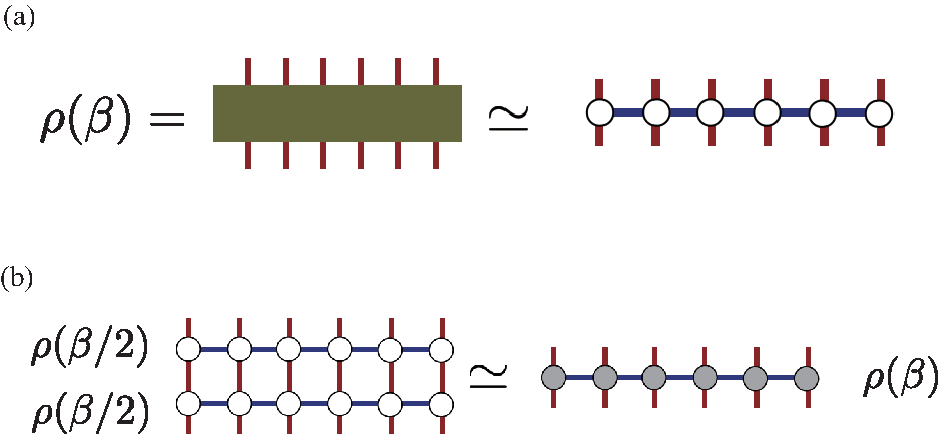
\includegraphics[width=\linewidth]{Figs/XTRG_MPO.pdf}
  \end{center}
  \caption{Tensor network diagram for the density operator approximation. (a) The density matrix is approximated as a %matrix product operator 
\red{MPO} with bond dimension $D$. %Here, t
\red{T}he horizontal line \red{in the right panel} corresponds to the gray line in Fig.~\ref{fig:lattice}(a). (b) The density matrix at $\beta$ is calculated as $\rho(\beta)=\rho(\beta/2)\rho(\beta/2)$. The bond dimension of the obtained $\rho(\beta)$ is truncated %to 
\red{at} $D$ through the standard optimization procedure of MPS.}
  \label{fig:XTRG}
\end{figure}

\subsection{Thermal pure quantum state}\label{subsec:Thermal pure quantum state}
%In this section
\red{Next}, we %explain 
\red{describe} the %basics of the canonical 
%thermal quantum pure (
\red{cTPQ} %) 
state method~\cite{Sugiura_PRL2013}, 
which enables us to calculat\red{e %the 
f}inite\red{-}temperature properties of quantum many-body systems using the power method. We note that several similar methods were independently proposed~\cite{Imada_JPSJ1986,Jaklic_PRB1994,Hams_PRE2000,Lloyd} before the proposal of the cTPQ \red{state} method~[\onlinecite{Sugiura_PRL2013}].
%We construct t
\red{T}he 
cTPQ state %$|\Phi_{\rm cTPQ}^{p}\rangle$ 
\red{is constructed} a\red{s} %follows:
\begin{align}
|\Phi_{\rm cTPQ}^{p}(\beta)\rangle = \exp\Big[-\frac{\beta}{2}\mathcal{H}\Big]|\Phi_{\rm rand}^{p}\rangle,
\end{align}
wher\red{e} %$\beta$ is inverse temperature and 
$|\Phi_{\rm rand}^{p}\rangle$ is the $p$th initial random vector, which is uniformly distributed
on the $N_{\rm H}$\red{-}dimensional hypersphere ($N_{\rm H}$ is the dimension of the Hilbert space of the given system).
Any local physical quantity at inverse temperature $\beta$
can be calculated as the expectation values of $|\Phi_{\rm cTPQ}^{p}(\beta)\rangle$, i.e.,
\begin{align}
\langle A(\beta)\rangle
=\frac{\langle \Phi_{\rm cTPQ}^{p}(\beta)|A|\Phi_{\rm cTPQ}^{p}(\beta)\rangle}
{\langle \Phi_{\rm cTPQ}^{p}(\beta)|\Phi_{\rm cTPQ}^{p}(\beta)\rangle}.
\end{align}
%In actual calculations, 
We numerically %construct 
\red{obtain} the cTPQ state %as follows:
\red{by} 
\begin{align}
%&
\exp\Big[-\frac{\beta}{2}\mathcal{H}\Big]|\Phi_{\rm rand}^{p}\rangle=U(\Delta\tau)^{k}|\Phi_{\rm rand}^{p}\rangle,%\\
\end{align}
\red{where $\beta=k\Delta\tau$ and}
\begin{align}
%&
U(\Delta\tau)=\exp\Big[-\frac{\Delta\tau}{2}\mathcal{H}\Big]\sim\sum_{n=0}^{n_{\rm max}}\frac{1}{n!}\left(-\frac{\Delta\tau}{2}\mathcal{H}\right)^{n}\red{.} %,\\
\end{align}
%&\beta=k\Delta\tau%,
%\end{align}
%where 
\red{In the following calculations,} we take $n_{\rm max}=6$ and $\Delta\tau =0.02$\red{, %in this paper
for which we confirm good convergence of} 
%We confirm that $n_{\rm max}=6$ ($\Delta\tau=0.02$) is sufficiently
%large (small) %for obtaining 
%to obtain converged 
physical quantities
in the calculated temperature region.
In actual calculations, we use $\mathcal{H}\Phi$~\cite{Kawamura_CPC2017,HPhi_v2,HPhi_release}, 
where the cTPQ \red{state} method is implemented.

The cTPQ \red{state} method %gives 
provides the numerically exact
results within the statistical %fluctuations
\red{errors},
which are defined by the statistical distribution of the initial random vectors.
To %evaluate 
estimate the statistical errors %fluctuations, i.e., the errors
of the cTPQ method, 
we employ the bootstrap method~\cite{HPhi_v2}.
%[\orange{bootstrap法の良い文献があれば引用してください。
%HPhi論文に具体的にprocedureを書いたのでとりあえずそれを引用しています。}
%\red{$\to$モンテカルロ法の教科書とかでBootstrap法の説明が載っていたりしますが、今の\cite{HPhi_v2}より適しているかと言えばそうでもない気がするので、今の引用が最適な気がしました。}].
%Using the bootstrap method~[\orange{cite a standard textbook}], we evaluate the average values and 
%error bars of physical quantities.
%The 
Benchmark results of the cTPQ \red{state} method in the pure Kitaev model are 
shown in Appendix \ref{app:cTPQ}. We also %show 
compare %the comparison between 
\red{the results of the cTPQ state method with those of} the XTRG metho\red{d %and 
%with the cTPQ method 
i}n Appendix \ref{app:XTRGcTPQ}.

\subsection{Classical Monte Carlo simulation}\label{subsec:Classical Monte Carlo simulation}
Finally, we %show the details of 
\red{describe} the \red{method of} classical Monte Carlo simulations.
In this method, an $S=1/2$ spin at each site is regarded as a classical vector \red{with length $1/2$}.
%Namely, 
%Specifically, a 
\red{The} classical spin at site $i$ is parameterized by $\theta_i$ and $\phi_i$ as
$\bm{S}_i = \frac{1}{2}(\sin\theta_i\cos\phi_i, \sin\theta_i\sin\phi_i, \cos\theta_i)$.
In the calculation\red{s} of the thermal average, the integral $\int \prod_i d\phi_i d\theta_i \sin\theta_i$ is evaluated %by 
using the Markov-chain Monte Carlo method.
To accelerate %the computation speed 
computations and avoid trapping %the 
spin configurations %at 
in local minima, we use the replica exchange method \cite{Hukushima1996}.
In the simulations, we prepare 48 replicas with different temperatures.
We perform 10~000~000~MC steps for measurements after 10~000~MC steps for thermalization in the 800-site cluster with %$L=10$ and $L'=40$
\red{$(L, L') = (10, 40)$.} 
%[see Fig.~\ref{fig:lattice}(a)].
%\blue{
The temperature derivative of $\langle O \rangle$ is evaluated by the correlation with ${\cal H}$ as  %$
\begin{align}
\red{\frac{d\langle O \rangle}%/
{dT}=\frac{%\left(
\langle O %A
{\cal H}\rangle -\langle O %A
\rangle \langle {\cal H}\rangle} %\right)/
{T^2},} %$. 
\end{align}
\red{which gives accurate estimates compared to numerical differentiation.} 
%, %while 
%\orange{whereas in quantum systems,} it is computed \orange{using numerical differentiation.}
%\red{[whereas 以降は量子系のところに書いたので、削除して良い気がしました。]}
%as a numerical difference 
%in the case of the quantum system.
%[要確認]\red{(この記述通りで、数値微分でOK。量子系のところにちゃんと説明を書く。$\to$書いた。)}
%}

%\clearpage
\section{Result}\label{sec:Results}
\red{In this section, ...}

\subsection{Pure Kitaev model}
\label{sec:pureKitaev}
\subsubsection{Magnetic fi%le
\red{el}d along [111] direction}
We %first discuss the temperature dependence of the
%physical quantities, including the thermal Hall conductivity $\kappa_{xy}$ of the 
%the case where 
\red{begin with the} ferromagnetic Kitaev model %is 
\red{($K=-1$ and $\Gamma = \Gamma^\prime = 0$)} 
%under a 
\red{in an applied} magnetic field %parallel to 
\red{along} the $[111]$ direction \red{($h^x=h^y=h^z$)}. 
In this setup, we expect %positive 
$\kappa_{xy}/T$ to be \red{quantized at a} positive \red{value of $\pi/12$} 
for small magnetic fields $h = |\vec{h}|$ in 
the zero temperature limit~\cite{Kitaev2006}. 
%
Fig\red{ures}%.
~\ref{fig:CMF_pure}(a)-\ref{fig:CMF_pure}(c) show the temperature dependence of 
the specific heat 
$C$, the magnetic moment along the magnetic field $M_{\parallel}$, and the flux density $W$, %which are 
%defined as 
\red{respectively} given by
\begin{align}
C&=\frac{\ev*{{\cal H}^{2}}-\ev*{{\cal H}}^2}{T^2}\red{,} \label{eq:C}\\
M_{\parallel}&=\ev*{\vec{M}}%\vec{M}
\cdot\frac{\vec{h}}{|\vec{h}|},~~\vec{M}=\frac{1}{N_{\rm s}}\sum_{i}\vec{S}_{i}\red{,} \label{eq:Mag}\\
W&=\frac{1}{N_{\rm h}}\sum_{p}\ev*{W_{p}}, %W_{p},
~~W_{p}=2^6\prod_{i\in p}S^{\gamma_{i}}_{i} \label{eq:W},
\end{align}
where $p$ runs over all hexagons in the honeycomb lattice and $N_{\rm h}$ is the number of hexagons\red{;} %. 
$\gamma_{i}$ %represents 
denotes the bond component %not belonging to 
that does not belong to the edges of $p$ at site $i$.

%\orange{where $p$ runs all hexagons in the honeycomb lattice and
%$\gamma_{i}$ represents the bond component 
%not belonging to the edges of $p$ at site $i$.}
%for various magnetic fields. 
%{\bf \orange{definition of W should be modified}}.

\red{We first discuss the temperature dependence of the specific heat $C$.} 
As shown in Fig.~\ref{fig:CMF_pure}(a),
%We see 
we %find 
observ\red{e %that 
c}lear double-peak structure\red{s %for each magnetic field which is considered to be 
%appear 
a}t each magnetic field, which %is 
\red{appear to evolve smoothly from the} 
%a 
characteristic %behavior 
feature of the Kitaev model \red{at zero field arising from fractionalization of spins into Majorana fermions}~\cite{NasuUM2014,NasuUM2015}.
%a characteristic of 
%\orange{This double peal structure is a signature of the two different energy scales, i.e.,  
%the localized and the itinerant Majorana fermions~\cite{NasuUM2014,NasuUM2015}.. } 
%the separation of energy scales of localized and mobile Majorana fermions \
By increasing the magnetic field, %we find that 
the low-temperature peaks %move 
shift to higher temperatures, while the high-temperature peaks are almost independent of the magnetic field. 
Th\red{is} %e sensitive 
behavior of the low-temperature peak %with respect to the magnetic field has 
\red{is not} %been 
observed in the calculations where the magnetic field is introduced perturbatively~\cite{NasuYM2017}, suggesting %that 
\red{the importance of} non-perturbative effects\red{.} %of the magnetic field 
%are important even in this low magnetic field regime.

%This tendency is understood from the local flux degrees of freedom are sensitive to the magnetic field.
%\red{(三澤さんへ:後半の文が正しいか判断できませんでした。少し直感に反している気もします。)}
%\orange{確かにflux gap以下の磁場なら比熱に変化はないはずですね。
%磁場を摂動で入れた那須さんの計算では2nd peakも磁場にたいして鈍感ですね。とりあえず磁場の非摂動効果だろうと言及するにとどめました。
%エッジがあることも影響しているかもしれないですね。}
%The low-temperature peaks move to higher temperature as we increase the magnetic field, while the high-temperature peaks are almost independent on the magnetic field. 
%\blue{[この比熱に関する議論は、吉竹君の論文J. Yoshitake et al, Phys Rev B 101, 100408 (2020)に基づいて議論すべきかもしれません(低磁場・低温の振る舞いをreliableでないと言い切ってよいのかどうか)。次の段落と関係しますが、比熱を見ると0.01から0.02にかけてピーク温度が減少しますが、これが吉竹論文の磁場によるQSLの抑制に見えます、より高磁場でのピークの高温へのシフトは低温が吉竹論文でいうforced ferroに対応するのかもしれないと思いました。
%その場合、どの程度言ってよいかわかりませんが、$\kappa_{xy}/T$のovershootingはforced ferroを反映したものの可能性もあるかもしれないですので、このあたりは、紙面にする前に議論する必要があるかもしれません。
%  ]}\red{$\to$ 議論希望です。}

%At a 
\red{In the} low\red{-field region for} %magnetic field (
$h\lesssim 0.03$\red{,} %), 
%we find that non-smooth temperature dependencies appear in the specific heat at low temperatures. 
the specific heat exhibits non-smooth temperature dependence at low temperatures. The origin of thi\red{s %non-smooth 
b}ehavior might b\red{e %the effects of originate from 
t}he finite bond dimensio\red{n %s 
$D$ in the XTRG calculations}. %However
\red{Nevertheless}, the magnetic-field dependence of the low-temperature peak %seems 
\red{appears} to be consistent with the %privious 
previous studies~\cite{YoshitakeNKM2020,LiZWWGQLGL2021,LiLXGQLS2024}, where th\red{e %low-temperature 
p}eak moves toward a lower temperature %by 
under a weak magnetic field, while it %moves 
shifts toward a higher temperature a\red{s %we increase 
t}he %magnec filed 
magnetic field \red{is increased to} %for 
$h %> h_c \sim 
\red{\gtrsim} 0.02$.
\red{The Kitaev model is known to exhibit a quantum phase transition from a topological chiral spin liquid to a polarized state at $h_c \simeq 0.02$~\cite{Jiang2011}. The above behavior may be associated with a signature of this transition.} 
%
%
%$D=500$. 
%\red{be due to the finite bond dimensions.}
\red{In contrast, in the higher-field region %F
f}or $h \gtrsim 0.04$\red{, %however, 
%the temperature dependence of 
t}he specific heat %is 
exhibits smooth temperature dependence down to $T=0.01$. 
Therefore, it is plausible that $D=500$ is sufficient to %discuss 
capture the thermal properties of the
Kitaev model %under a magnetic field
\red{in this field region}. 
%Additional 
Further discussions on the %bond-dimension 
\red{$D$} dependence are shown in Appendix~\ref{app:XTRG_Bench}.
%Although the slight non-smooth temperature dependencies for $h \lesssim 0.03$ is considered due to the small $D$ effect, the specific heats for $h \gtrsim 0.04$ is smooth and the present $D=500$ seems to be sufficient for discussing thermal properties of the model. Additional discussions on the bond-dimension dependencies are in App.~\ref{app:XTRG_Bench}.

\begin{figure}
  \begin{center}
    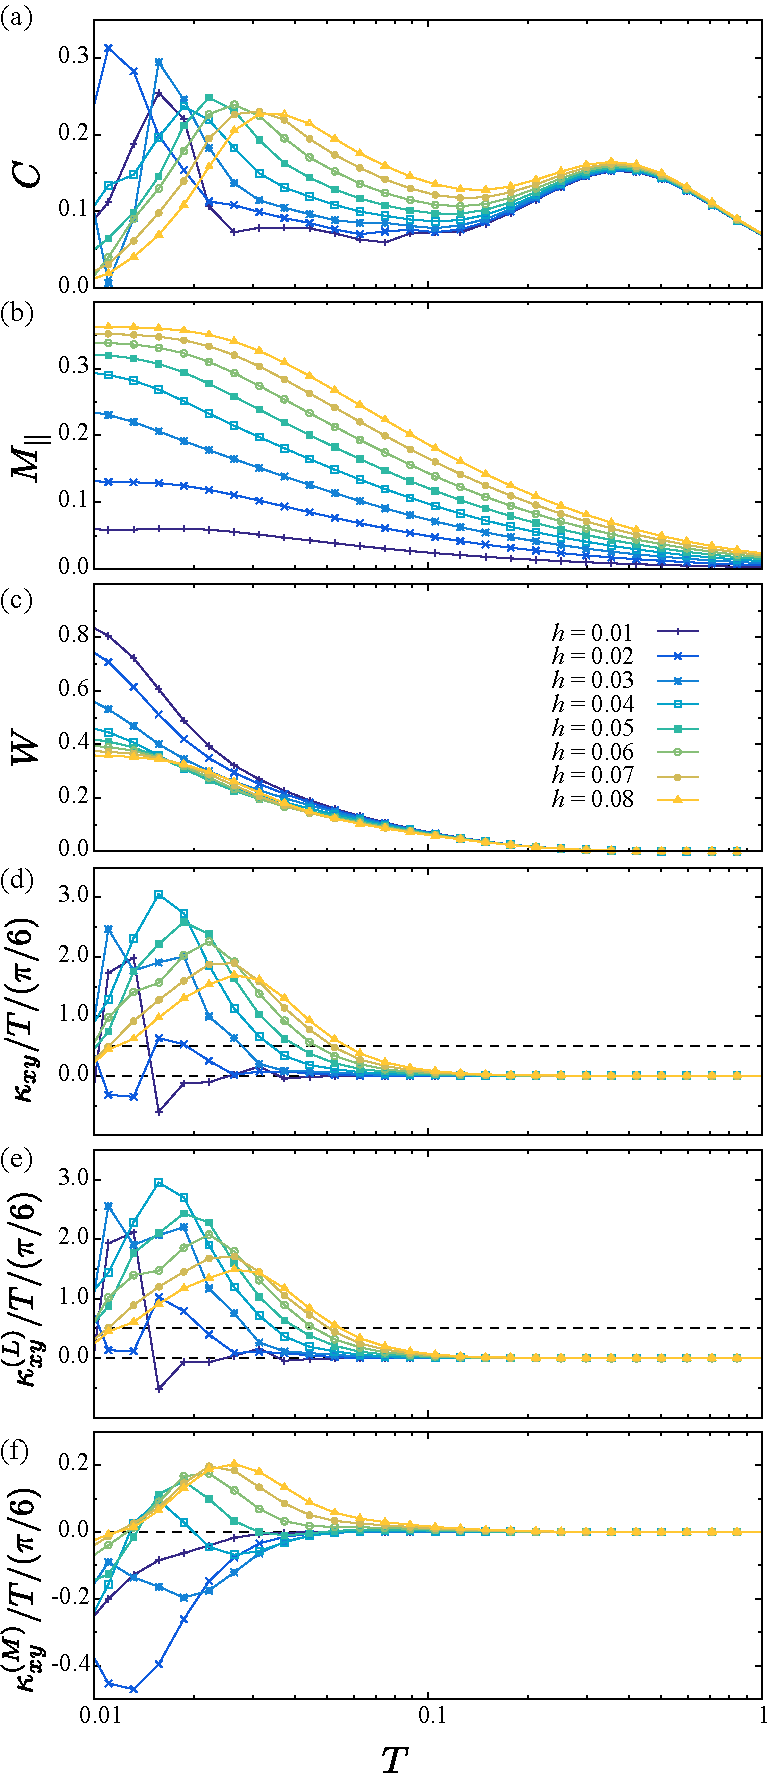
\includegraphics[width=0.9\linewidth]{Figs/plot_CMWkT.pdf}
  \end{center}
  \caption{Temperature dependence of (a) the specific heat \red{[Eq.~\eqref{eq:C}],} (b) the magnetic moment \red{[Eq.~\eqref{eq:Mag}],} (c) the flux \red{density [Eq.~\eqref{eq:W}]}, and (d) \red{the thermal Hall conductivity $\kappa_{xy}$ [Eq.~\eqref{eq:def_kxy}] divided by $T$} %$\kappa_{xy}/T$ 
of the ferromagnetic Kitaev model for %various 
\red{several values of the} external magnetic field parallel to the $[111]$ direction \red{($h=|\bm{h}|$)}. (e\red{), (}f) Contributions from the three-\red{spin term in Eq.~\eqref{eq:L}} %body ($L$) 
and the two-\red{spin} %body 
%($M$) 
ter\red{m %s 
in Eq.~\eqref{eq:M}} 
to $\kappa_{xy}/T$, respectively. \red{The data in (d), (e), and (f) are plotted in units of $\pi/6$, and %T
t}wo horizontal dashed lines \red{in each figure} indicate $\kappa_{xy}/T = 0$ and the half-\red{integer} quantized value \red{$\pi/12$}.
  }
  \label{fig:CMF_pure}
\end{figure}

%\blue{[magnetizationの定義が必要かと思います。$M_{111}$より、$\bm{M}=\frac{1}{N}\sum_i \bm{S}_i$として、$M_\parallel$を$M_\parallel=\bm{M}\cdot\bm{h}/|\bm{h}|$と定義した方がよいかもしれません。]}\red{この提案を採用します。}


\begin{figure*}[htb]
  \begin{center}
    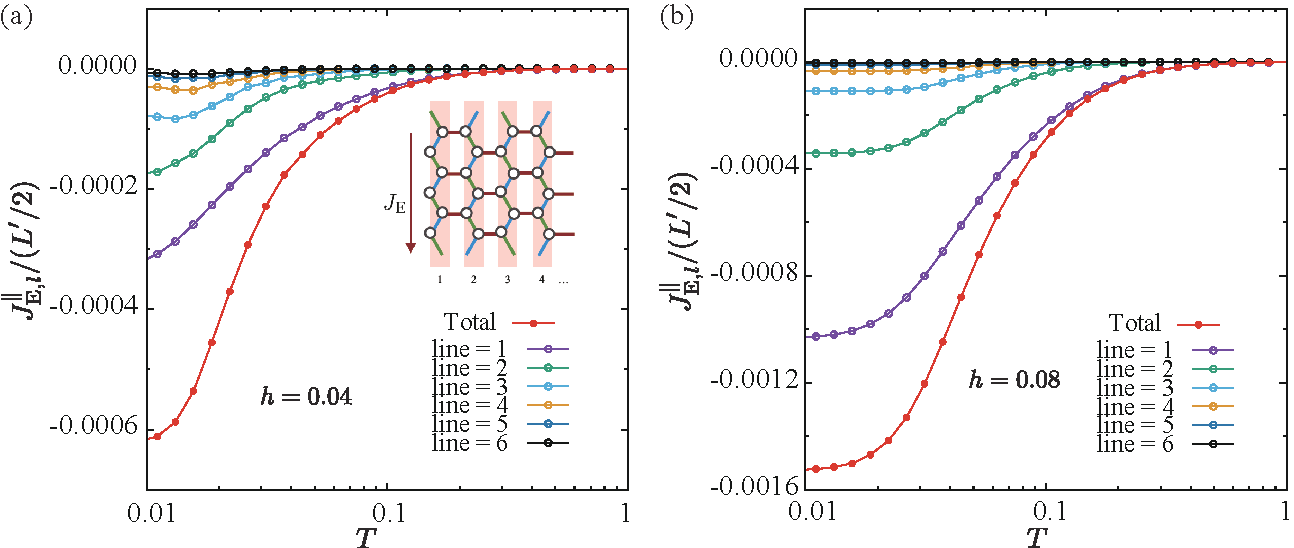
\includegraphics[width=0.9\linewidth]{Figs/J_line_all.pdf}
  \end{center}
  \caption{Temperature dependence of the energy current of the ferromagnetic Kitaev model %under 
\red{at} (a) $h=0.04$ and (b) $h=0.08$. In addition to the total energy current, the contribution from each line is shown\red{; see Eq.~\eqref{eq:JE}}.
\red{[need ``$\langle \cdots \rangle_T$" in the labels on the vertical axes? also need the label ``$\langle J_{\mathrm{E}}^\parallel \rangle_T/(L^\prime/2)$"?]} 
}
  \label{fig:J_line}
\end{figure*}

Next, we %next 
discuss the temperature dependence of the magnetization \red{$M_\parallel$} and the flux density \red{$W$ shown in Figs.~\ref{fig:CMF_pure}(b) and \ref{fig:CMF_pure}(c), respectively}. 
As expected, by increasing the magnetic field, 
%the magnetic moment 
\red{$M_\parallel$} monotonically increases, %and it reaches
reaching more than 60\% of the saturation value of %magnetization 
\red{$0.5$ %at $h=0.08$ and $T=0.01$. 
for $h\gtrsim 0.05$ at low temperatures}. 
Since an applied magnetic field inducing nonzero magnetization renders %a 
the flux operator on each hexagonal plaquette a nonconserved quantity, %the finite magnetization destroys the flux,
%the flux density %fluxes
\red{$W$} monotonically decreases by increasing the magnetic field\red{, %.
%At $h=0.08$, the flux density $W$ is about 
down to $\sim 0.4$ for $h\gtrsim 0.05$} at low temperatures, 
which is significantly %reduced from 
lower than $W=1$ \red{expected for} %in 
the ideal Kitaev QSL\red{.
%As we show later, even %at 
%in this high-magnetic region,
%the thermal Hall conductivity still remains large.
W}e note that %there is a phase transition between a %the 
%chiral spin liquid and the paramagnetic phase 
\red{both $M_{\parallel}$ and $W$ decrease rapidly around at} 
%around 
$h_c \simeq 0.02$\red{.} %\cite{ZhuKSF2018,LeeKCOYKK2020}. 
%However, in the present calculations, 
%we do not observe a clear singularity indicating %corresponding to
%the 
%a phase transition possibly due to finite size effects or because the calculation has not been 
%carried out 
%performed at %to
%sufficiently low temperatures to %observe 
%detect its signatures.
%For such $h \gtrsim 0.04$ at low temperature, the magnetizations are slightly high as $M_{111} \ge 0.3$ (Fig.~\ref{fig:CMF_pure}(b)), and also the fluxes are $W \ge 0.4$ (Fig.~\ref{fig:CMF_pure}(c)), which is smaller than $W=1$ expected for the zero magnetic filed. 

%\orange{Fig.3 (d)-(f)の説明の前にFig.4の説明がはいるのはおかしいので、
%このあとの2段落はこのsectionの最後にもっていく?}\red{[$\to$ 個人的には、Fig.3(d)-(f)の説明の前に、Fig. 4の話があるのは、OKな気がします。議論の流れ的にも、そちらの方が自然な気がしているので、現在の構成のママが良いと思いました。]}
\red{Figure~\ref{fig:CMF_pure}(d) displays the temperature dependence of the thermal Hall conductivity divided by temperature, $\kappa_{xy}/T$. 
As this is obtained by the temperature derivative of the energy current through Eq.~\eqref{eq:def_kxy} with Eq.~\eqref{eq:JE}, let us discuss the behavior of the energy current first. 
%In Fig.~\ref{fig:J_line}, we show 
Figure~\ref{fig:J_line} shows the temperature dependence of} the total energy current \red{$\langle J_{\mathrm{E}}^\parallel \rangle_T$} defined in Eq.~\eqref{eq:JE} 
at two representative magnetic fields, $h=0.04$ and $h=0.08$. 
We find that %the energy currents 
\red{$\langle J_{\mathrm{E}}^\parallel \rangle_T$} monotonically decrease\red{s} 
%as a function of the temperature 
%with 
\red{while} decreasing temperature, starting from $\langle J_{\mathrm{E}}^{\parallel} \rangle_T %J_{E}^{\parallel}
=0$ in the high-temperature limit. This behavior indicates that $\red{\kappa_{xy}}%=d %\langle J_{\mathrm{E}}^{\parallel} \rangle_T %J_{\mathrm{E}}^{\parallel}
%/d T
$ 
is positive \red{in the entire temperature range}, %and 
which is consistent with the expectation %of 
in the zero temperature limit. 
\red{In addition, $\langle J_{\mathrm{E}}^\parallel \rangle_T$ exhibits an inflection point at an intermediate temperature, indicating that $\kappa_{xy}$ has a peak at the corresponding temperatures, as discussed below. 
Notably, the temperature of the inflection point appears to correlate with the peak temperature of the specific heat in Fig.~\ref{fig:CMF_pure}(a).} 

%To examine the spatial distribution of the energy current,
%we also plot the position-dependent energy current in Fig.~\ref{fig:J_line}. 
\red{Figure~\ref{fig:J_line} also plots the contributions from each zigzag chain, $\langle J_{\mathrm{E},l}^\parallel \rangle_T$. 
We find that the amplitude of the energy current i\red{s %the 
l}argest at the edge ($l=1$), and rapidly decreases toward the center of the system ($l=6$) [see Fig.~\ref{fig:lattice}(a)].} 
%When we go
%By changing its position
%from the edge %side 
%($l=1$) to the center ($l=6$), 
%the amplitude of the energy current decreases.
This result demonstrates that the %edge 
\red{energy} current %mainly contributes
%to the thermal Hall conductivity %. 
\red{is dominated by} 
%The dominant contribution of 
the edge current\red{,  %also 
%indicates that the nonzero thermal Hall conductivity %\blue{reflects} %is dominated by
similar to the chiral edge current} 
originat\red{ing} %es 
from
the topological\red{ly-nontrivial Majorana band structure predicted by the perturbation theory.} %nature of the excitation structure. %properties. 
%Because the contributions from the center region are sufficiently small, 
%we consider that our total energy current $J_{\mathrm{E}}$, 
%which is the sum of contributions from all lines up to centers, 
%correctly captures the edge current. 
\red{Note that the contributions from the center region are sufficiently small, indicating that the employed system size, $L=6$, is large enough to capture the essential features of this edge current. 
Interestingly, we observe the edge current even for high fields well beyond $h_c \simeq 0.02$.} 
We also %realize 
find that %the decay of 
the current amplitude decays more rapidly toward the center %becomes faster 
%when we increase 
\red{as} the magnetic field \red{increases}. 
This behavior might be explained by the increase in the excitation gap of quasiparticles carrying energy. %the energies. 
%Since the contributions from the center region are sufficiently small, 
%the employed system size, $L=6$, %that we employ 
%is %sufficiently 
%large enough to capture the %essence 
%essential features of the thermal Hall conductivity.
%which is the sum of contributions from all lines up to centers, 
%correctly captures the edge current. 


%Here, we 
\red{Then, let us} discuss the temperature dependence of %the thermal Hall conductivity
\red{$\kappa_{xy}/T$ shown in Fig.~\ref{fig:CMF_pure}(d).} 
%by evaluating %taking
%the numerical derivative of {$J_{\mathrm{E}}^{\parallel}$}, i.e., $\kappa_{xy}=d {\ev*{J_{\mathrm{E}}^{\parallel}}}/dT$.
%we obtained the thermal Hall conductivity as Eq.~\ref{eq:def_kxy}. 
%Thus o
%The obtained values of  %Obtained 
%$\kappa_{xy}/T$ are shown in Fig.~\ref{fig:CMF_pure}~(d). 
\red{First of all, $\kappa_{xy}/T$ is overall positive, except for small $h$ and low $T$,  
%Except for small magnetic fields, we %see 
%observe 
and exhibits a nonmonotonic temperature dependence with} a clear peak structure\red{, which} %in Fig.~\ref{fig:CMF_pure}~(d): for example,
%the peak appears around $T=0.02$ for $h=0.05$. 
%The peak temperatures %move 
shift\red{s} to %a 
higher temperature\red{s %side 
w}ith increasing %as we increase
$h$. 
\red{These behaviors are expected from $\langle J_{\mathrm{E}}^\parallel \rangle_T$ in Fig.~\ref{fig:J_line}.} 
%Moreover, the peak of $\kappa_{xy}/T$ develops with increasing $h$ up to $h=0.04$ and shifts to the high-temperature side.
% they seem to be
%\blue{They appear to be} 
%This behavior appears to be correlated with the low-temperature peaks of the specific heat. 
%Thus, this result indicates that $\kappa_{xy}/T$ around this temperature region is governed by the local flux degrees of freedom.\red{ここまで言い切れるのか不安です}
%\orange{なんで、これでflux degreeと関係しているのか確かによくわからないので、削除でいいかなと思います。}
%\red{削除しました}
%Interestingly
\red{Surprisingly}, \red{the peak of} $\kappa_{xy}/T$ %becomes much larger than 
\red{largely exceeds} the half-\red{integer} quantized valu\red{e %(%shown 
i}ndicated by the broken line \red{in Fig.~\ref{fig:CMF_pure}(d).} %) 
%for 
%at intermediate temperatures. 
\red{It appears to develop with increasing $h$ up to $h\simeq 0.04$ and slowly decline for higher $h$.} 
Such an overshooting behavior was not observed in the previous numerical calculations %on an effective model 
%with perturbative treatment of the magnetic fields~\cite{NasuYM2017}. 
which 
treated the magnetic fields as the effective three-\red{spin} %body 
interactions~\cite{NasuYM2017}, or defined \red{the} energy current in a simplified way~\cite{KumarT2023}. %\red{ここで、Kumarの計算にも言及した方が良い気がしたのですが、いかがでしょうか。} 
\red{Our results indicate that full quantum calculations with proper definition of the energy current can explain the overshooting behavior observed in experiments by purely magnetic origin, without considering contributions from phonons~\cite{Ye2018Quantization,Vinkler2018}.} 
\red{[should we comment on the relation to Joy2022?]} 

We note that %in 
\red{while $\kappa_{xy}/T$ takes a value around the half-integer quantization $\pi/12$ at} the low\red{est} %-
temperature %limit
\red{calculated, %we do 
it does} not %find 
\red{exhibits} any clear signature of the 
convergenc\red{e %of $\kappa_{xy}/T$ 
t}o the %half quantized value
\red{quantization,} even when the magnetic field is sufficiently small.
\red{This is presumably due to the finite bond dimension $D$, finite-size effects, and insufficiently low temperatures.} 
%the calculated $\kappa_xy/T$ does not converge to the half-quantized value. 
\red{First, %A
as %we 
d}iscussed \red{for the specific heat} above\red{, %for $h\lesssim0.04$, 
t}he bond dimension $D=500$ is not sufficient
to obtain reliable results %below $T=0.01$ 
\red{at low temperatures for $h\lesssim0.04$}.
%Moreover, due to the finite-size effects, %finiteness of the circumferential directions, 
%even for the sufficiently small $h$, 
\red{Second, for the finite-size effects, the excitation gap is expected to be smaller for smaller $h$, leading to a larger spatial extension of the edge current into the bulk. 
This causes an overlap between the contributions from both edges in the finite-size cluster, thereby hampering accurate estimates of the edge current.} 
%the %expected 
%chiral edge mode %has 
%might 
%is expected to have a finite gap.
%This finite-size gap might make 
%$\kappa_{xy}/T$ zero in the low-temperature limit.
%and then $k_xy/T$ becomes zero in the low temperature limit. 
\red{Lastly, asymptotic quantization is expected to occur for sufficiently lower temperatures compared to the excitation gap of topological quasiparticles, whose precise value is not known beyond the perturbation theory. 
Sophisticated methods are required to further study this issue.} 
%Thus, in the present calculations, 
%we do not %deeply discuss 
%further investigate the behavior %behaviors
%of $\kappa_{xy}/T$ at low magnetic fields ($h\lesssim0.02$) and low-temperature region ($T\lesssim 0.01)$,%($T\lesssim 0.05)$,
%where the effects of the finite bond dimensions and finite sizes become serious.
%\red{ここでの温度の意図は、$h= 0.02$くらいだと、$T < 0.05$の精度が信頼できないという気持ちの数字なのですが、今の書き方だと、他の磁場でも、$T < 0.05$はinvestigate しないように読み取れる気がしました。どう思われますか?}
%for lower temperatures. 

To gain more insights %on 
into the thermal Hall conductivity, 
we separate it into the two parts $\kappa_{xy}^{(L)}$ and  $\kappa_{xy}^{(M)}$, which are
% we calculate the
contributions from the three-\red{spin} %body 
an\red{d %the 
t}wo-\red{spin} %body 
correlations %as shown 
%in Figs.~\ref{fig:k_all_pure}(b) and (c), which are
defined in Eqs.~(\ref{eq:L}) and (\ref{eq:M}), respectively.
Figures~\ref{fig:CMF_pure}(e) and \ref{fig:CMF_pure}(f) %shows 
show the temperature dependence of $\kappa_{xy}^{(L)}$ and  $\kappa_{xy}^{(M)}$, respectively.
%In Figs.~\ref{fig:k_all_pure}(b) and (c), we plot the contributions from the three-body and the two-body correlations, respectively, to the total $\kappa_{xy}/T$. 
%We find that the three-body correlations 
%are the dominant contributions to $\kappa_{xy}/T$ for all magnetic fields. 
%Although the two-body correlations are less dominant, 
%quantitatively, we also see peak structure in them for $h \ge 0.04$.
We find that the three-\red{spin} %body 
part $\kappa_{xy}^{(L)}/T$  dominantly
%contribute
contributes
to the total $\kappa_{xy}/T$ %for 
across all magnetic fields.
% The peak positions of $\kappa_{xy}^{(L)}/T$ are also roughly consistent
% with those of $\kappa_{xy}/T$. 
In contras\red{t,} %to this, 
the %contributions 
contribution from two-\red{spin} %body 
part $\kappa_{xy}^{(M)}/T$
%are 
is an order of magnitude smaller than %those 
that from the three-\red{spin} %body 
part \red{and plays a minor role}.
%Moreover, $\kappa_{xy}^{(M)}/T$ become negative for small $h$ and low $T$ region.
% These results suggest that the thermal Hall conductivity is mainly governed by 
% the Majorana fermions with the finite Chern number. 
%\blue{Moreover, the peak of $\kappa_{xy}^{(L)}/T$ develops with increasing $h$ up to $h=0.04$ and shifts to the high-temperature side as shown in Fig.~\ref{fig:CMF_pure}(e).}\red{"Moreorver..."の文、元の修正では、$\kappa_{xy}/T$と書いてましたが、それだと意味が通らないので、$L$ termのことだと推測して修正しました。それでも、変な気がするので、この文章自体を削除したい気がしました。}\orange{確かに変ですね。}
%\blue{削除でも良いと思いますし、どこまでこの計算が妥当かという部分と関わってきますが、$h=0.04$までとそれ以上での違いに意味を見いだせれば、この領域も計算として妥当であれば$\kappa_{xy}/T$ [Fig.~\ref{fig:CMF_pure}(d)]として前の段落に入れても良いかもしれません。}
%\red{コメントありがとうございます。意図が分かりました。低磁場の$h=0.02$とか$h=0.03$の値については、あまり自信がないので、あまり強調しない感じが良いです。ですので、削除の方が、安心かもしれません。}

 %\blue{[$\kappa_{xy}^{(M)}$がマグノン由来かはわからない?たぶん正確には、Majorana formalismではthree-body的な部分が外場として入っているけれども、Magnon formalismでは、ここで考えている寄与はすべて含まれているはずなので、そのように書き直してみました。]}
% Here
\red{From these observations}, we discuss the origin of the thermal Hall effect.
Since the three-\red{spin} %body part 
terms \red{in Eq.~\eqref{eq:L} is represented by} %include 
the effective magnetic field obtained from the third-order perturbations for $\bm{h}$ \red{in the Majorana fermion representation},
 $\kappa_{xy}^{(L)}$ is expected to %be related to 
\red{include the contributions predominantly from} the topologica\red{l %Majorana 
g}ap \red{opening} in the emergent Majorana fermion system.
 In contras\red{t,} %to the three-body part, 
the two-\red{spin} %body part 
\red{terms in Eq.~\eqref{eq:M}} 
%  explicitly includes
% the amplitude of 
%\blue{is linear with} 
scal\red{e} %s 
linearly with the magnetic field\red{, suggesting} %. 
%Thus, it is expected that $\kappa_{xy}^{(M)}$ may contain the effects of the magnons.
%This indicates 
that $\kappa_{xy}^{(M)}$ %is caused by 
\red{includes} effects beyond %noninteracting 
\red{the} Majorana fermion picture, which
may %contain contributions from %the effects of the
\red{be better described by} magnon \red{excitation}s.
\red{Since $\kappa_{xy}$ is dominated by $\kappa_{xy}^{(L)}$ as discussed above, 
%The low-field 
its} behavior \red{in the calculated field range} is consistent\red{ly understood by} %with 
the \red{topological} Majorana fermion picture %where the topological property %becomes rigid 
%is stabilized by an applied magnetic field %, but it cannot be accounted for by 
\red{rather than} the magnon picture\red{. 
Note that the magnon contributions} %where the absolute value of $\kappa_{xy}/T$ 
should monotonically decrease %by applying 
with increasing the magnetic field~\cite{McClarty_PRB2018}.
Our results suggest that Majorana-like excitations %dominantly contribute to 
play a dominant role in the thermal Hall effect %via the three-body spin part $\kappa_{xy}^{(L)}$.
\red{exhibiting a large peak at an intermediate temperature, in a wide range of the magnetic field even beyond $h_c \simeq 0.02$.} 
%\red{ここでの記述は、一つ前の段落のコメントと関連しているのかなと思いました。Zoomで議論できれば。}
%{\bf \orange{この結論は唐突?もう少しthree-body = Majorana起源、
%two-doby= magnon起源などの議論をする必要?}}\blue{[少し表現を変えてみました。]}
%Although the two-body correlations are less dominant, 
%quantitatively, we also see peak structure in them for $h \ge 0.04$.

% \begin{figure}
%   \begin{center}
%     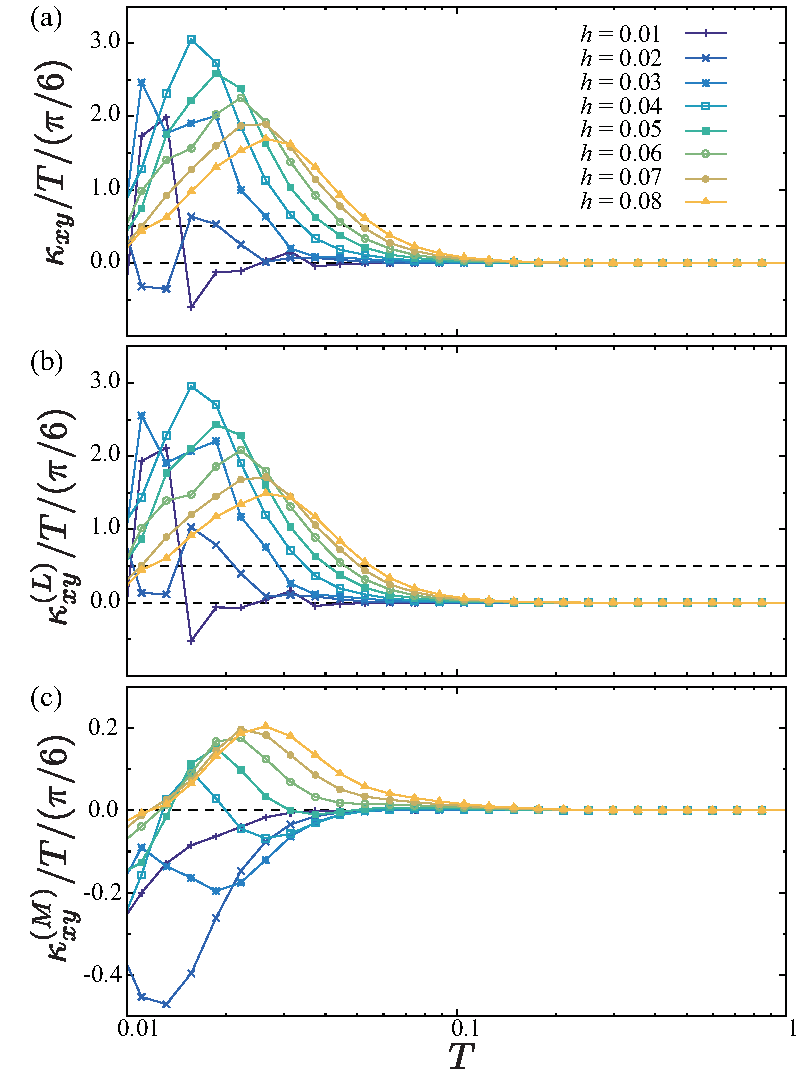
\includegraphics[width=0.9\linewidth]{Figs/plot_k_all.pdf}
%   \end{center}
%   \caption{\textcolor{red}{(To be updated)}(a) Temperature dependence of $\kappa_{xy}/T$ of the ferromagnetic Kitaev model for various magnetic fields parallel to the $[111]$ direction. Two horizontal dashed lines indicate $\kappa_{xy}/T = 0$ and the half-quantized value. (b,c) Contributions from the three-body ($L$) and the two-body ($M$) terms, respectively.}
%   \label{fig:k_all_pure}
% \end{figure}


\subsubsection{Field-\red{direction} %angle 
dependence}



\begin{figure}[htb]
  \begin{center}
    % 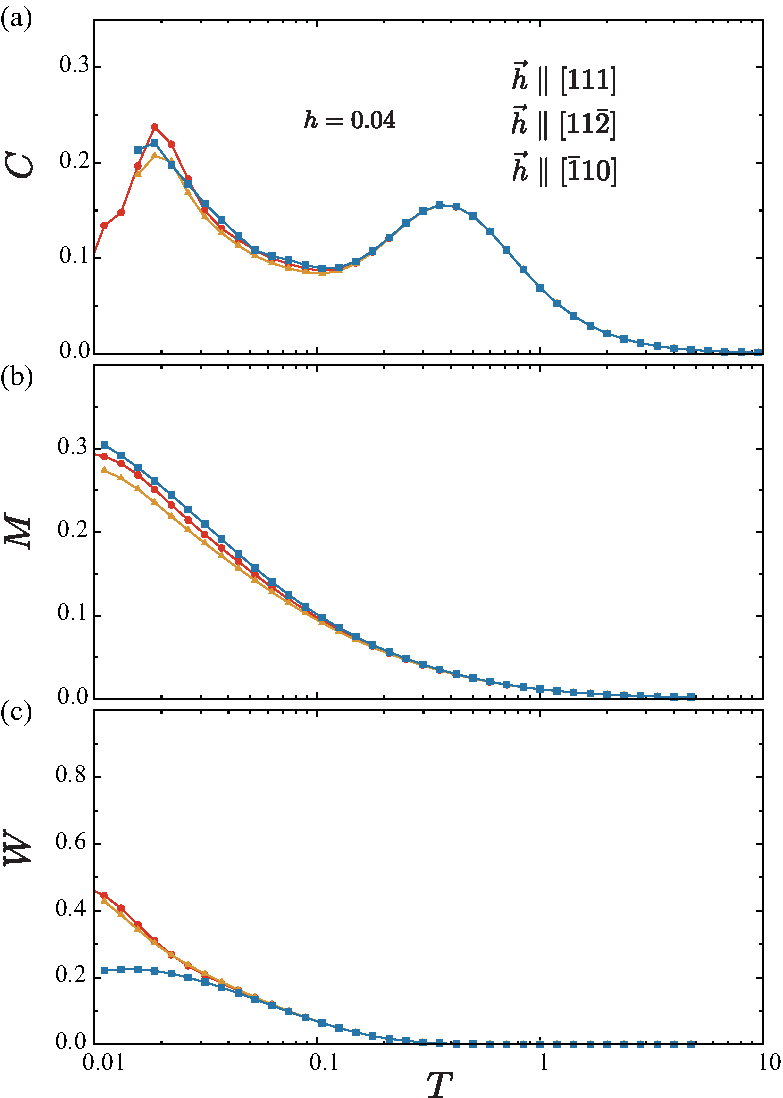
\includegraphics[width=0.9\linewidth]{Figs/plot_CMF_h0.04_ab.pdf}
    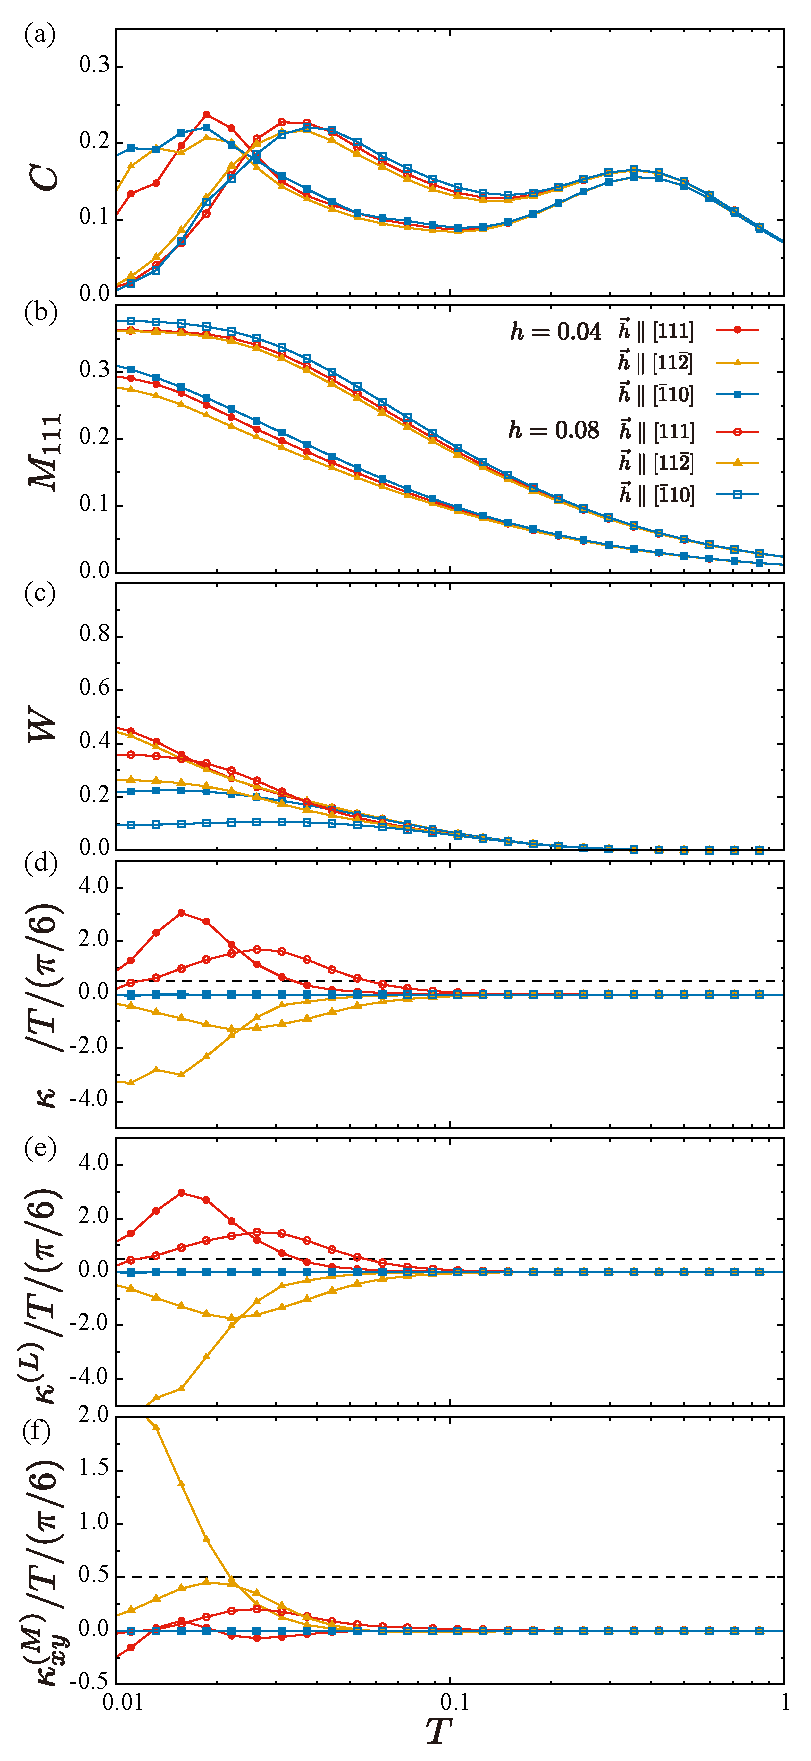
\includegraphics[width=0.9\linewidth]{Figs/plot_all_ab.pdf}
  \end{center}  
  \caption{Temperature dependence of (a) the specific heat\red{,} (b) the magnetic moment\red{,} (c) the flux, and %,
\red{(}d) $\kappa_{xy}/T$ of the ferromagnetic Kitaev model under magnetic fields parallel to $[111]$, $[11\bar{2}]$, and $[1\bar{1}0]$ with $%|
\red{h}%|
=0.04$ and $%|
\red{h}%| 
= 0.08$. (e),(f) Contributions from the three-\red{spin term in Eq.~\eqref{eq:L}} %body ($L$) 
and the two-\red{spin term in Eq.~\eqref{eq:M}} %body ($M$) terms 
to $\kappa_{xy}/T$, respectively. %Two 
\red{The data in (d), (e), and (f) are plotted in units of $\pi/6$, and the} horizontal dashed lines indicat\red{e %$\kappa_{xy}/T = 0$ and 
t}he half-\red{integer} quantized value \red{$\kappa_{xy}/T = \pi/12$}. 
  %\blue{[b軸で低温での比熱のデータが切れている理由は何かあるでしょうか。b軸でエントロピーが残りやすいような振る舞いがあれば実験と関係するかもしれません。]$\to$ [大久保さんが追計算してくださることになりました]}\red{[$\to$ これって、結局本文では特に触れてない気がしますが、議論を追加した方が良いでしょうか?]}
  }
  \label{fig:CMF_ab}
\end{figure}
% \begin{figure}[htb]
%   \begin{center}
%     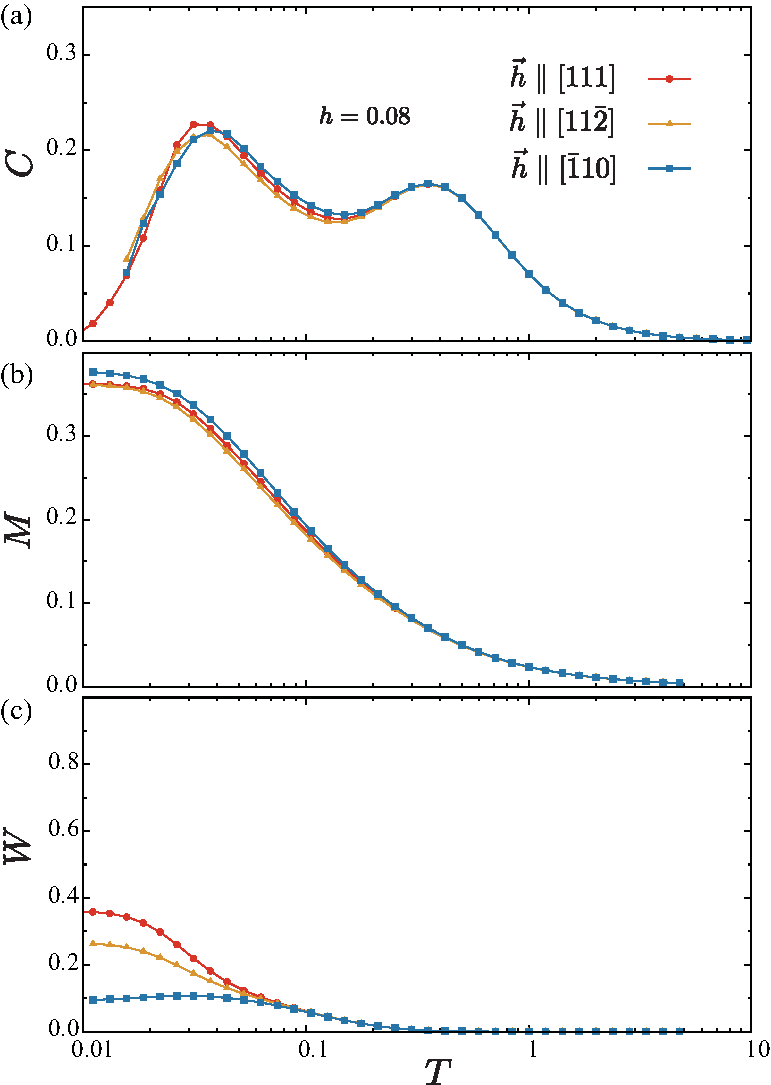
\includegraphics[width=0.9\linewidth]{Figs/plot_CMF_h0.08_ab.pdf}
%   \end{center}
%   \caption{Corresponding plot to Fig.~\ref{fig:CMF_h0.04_ab} for $|h|=0.08$.}
%   \label{fig:CMF_h0.08_ab}
% \end{figure}

%\blue{[Appendix Dをここに持ってきました。Fig.6,7は8,9と統合してもよいかもしれません。]}
In this section, we examine the field-\red{direction} %angle 
dependence of physical quantities in the pure Kitaev model.
\red{Here we consider three cases by taking the magnetic field direction parallel to [$111$], [11$\bar{2}$], and [$\bar{1}$10]. 
Note that the data for [$111$] are common to those in the previous section. 
When we take the $(S^x, S^y, S^z)$ axes to the cartesian coordinates connecting the magnetic ion and the surrounding ligands in the edge-sharing honeycomb network of octahedra~\cite{Jackeli_PRL2009},  the [$111$] direction is out-of-plane, while [11$\bar{2}$] and [$\bar{1}$10] are in-plane.} 
\red{[better to show the figure?]} 
%We show the filed-angle dependence of 
%physical quantities for $h=0.04$  ($h=0.08$) in Fig.~\ref{fig:CMF_h0.04_ab} (Fig.~\ref{fig:CMF_h0.08_ab}). 
\red{The perturbation theory for the magnetic field predicts changes in the band topology in the Majorana fermion bands: the gap in the Majorana excitations opens in proportion to the product of three field components $h^x h^y h^z$, and the Chern number $\nu$ changes its sign depending on the sign of $h^x h^y h^z$~\cite{Kitaev2006}. 
This suggests that $\kappa_{xy}/T$ in Eq.~\eqref{eq:k_xy} changes its sign depending on the sign of $h^x h^y h^z$. 
For instance, $\kappa_{xy}/T$ is expected to be positive and negative for the [$111$] and [$11\bar{2}]$ fields, respectively, whereas it vanishes for [$\bar{1}10$].
We examine such behaviors by numerics beyond the perturbation theory.} 

Figure~\ref{fig:CMF_ab} shows the results for  $h=0.04$ and $h=0.08$. 
We find that the specific heat and the magnetization do
not show significant changes %among 
across different \red{field} directions \red{as shown in Figs.~\ref{fig:CMF_ab}(a) and \ref{fig:CMF_ab}(b)}, %while 
whereas the flux \red{density} significantly decreases
for the [$\bar{1}$10] direction \red{as shown in Fig.~\ref{fig:CMF_ab}(c)}. This behavior 
%can be understood from the fact that the Majorana gap is zero for [$\bar{1}$10] direction.
might be related to the presence of low-energy %fluctuations 
\red{excitations, as the gap does not open in the Majorana excitations for the field in this direction in the perturbation theory~\cite{Kitaev2006}.} %due to the gapless Majorana dispersion for [$\bar{1}$10] direction. 
%[表現を弱めてみましたがこれでも微妙かもしれません。]

%While thermodynamic quantities such as the specific heat and the magnetization %is
%are insensitive for the field direction, t
\red{T}he thermal Hall conductivity %shows 
\red{exhibits} strong field-\red{direction} %angle 
dependence\red{, as expected in the perturbation theory}.
\if0{
We examine the field-angle dependence %in 
of $\kappa_{xy}$. 
If the Majorana fermions or topological magnons govern the thermal Hall conductivity,
$\kappa_{xy}$ should change its sign %according to the 
depending on the directions of the magnetic field
since the sign of the Chern number depends on the magnetic field direction.
%s of magnetic fields.
For example, %it is expected that 
$\kappa_{xy}$ %becomes 
is expected to be positive (negative) for the [111] magnetic field, %while
whereas $\kappa_{xy}$ becomes negative (positive) for the [11$\bar{2}$] magnetic field in the wide temperature region for the case of Majorana fermion (topological magnon) picture~\cite{McClarty_PRB2018, Joshi_PRB2018, ChernZK2021}.
%, and $\kappa_{xy}$ becomes zero for [$\bar{1}$10] magnetic field.
We %will 
examine whether $\kappa_{xy}/T$ satisfies these
%direction 
directional dependencies in the original spin representation. %by picking up two representative magnetic fields, $h=0.04$ and $h=0.08$.}
%Here we pick up two representative magnetic fields, $h=0.04$ and $h=0.08$, and consider three directions of magnetic fields as $\vec{h} \parallel [111]$, $[11\bar{2}]$, and $[\bar{1}10]$. 
% \orange{We confirm that the field-dependence of the bulk physical quantities other than the flux is small, which is shown in Appendix~\ref{app:fieldangle}.}
}\fi
%Figures~\ref{fig:CMF_ab}(d)--\ref{fig:CMF_ab}(f) show the temperature dependence of $\kappa_{xy}/T$ for three magnetic-field directions at $h = 0.04$ and $h=0.08$. %We see that the change of the field direction from $\vec{h}
% \orange{As expected}, 
%By changing the direction of the magnetic field from $\vec{h}\parallel [111]$ to  $\vec{h}\parallel [11\bar{2}]$, 
\red{As shown in Fig.~\ref{fig:CMF_ab}(d), we find that} 
$\kappa_{xy}/T$ %changes the sign %of $\kappa_{ky}$
reverses its sign
from positive to negative \red{by changing the field direction from [$111$] to  [$11\bar{2}$]}. 
We also find that the three-\red{spin contribution} %body part 
$\kappa_{xy}^{(L)}$ is dominant and governs the sign \red{change} of the total $\kappa_{xy}$ in both cases\red{. %In the $\vec{h}\parallel [11\bar{2}]$ case,
%$\kappa_{xy}^{(M)}$ becomes negative but remains small for $h=0.04$. %and $h=0.08$.
% This result is consistent with the three-body part being related to the topological properties, i.e., the Chern number while the two-body part is not. 
In addition, $\kappa_{xy}/T$ is vanishingly small for [$\bar{1}11$]. 
T}hese results suggest that the \red{topological} Majorana fermion picture %is rather plausible 
provides a plausible explanation for 
%explaining 
the field-\red{direction} %angle 
dependence of the thermal Hall effect %in addition to the field-intensity dependence.
\red{in the wide range of the field intensity beyond the perturbative region}. 
%[表現を少し変えてみました]
%such sign change can be seen also in the contributions from the three-body correlations, while we do not find clear corresponding behavior in the contributions from the two-body correlations. In particular, in the case of $h = 0.08$, both of $\kappa^{(M)}_{xy}/T$s show positive peaks for $\vec{h} \parallel [111]$ and $\vec{h} \parallel [11\bar{2}]$. Note that, in the case of $\vec{h} \parallel [\bar{1}10]$, $\kappa_{xy}/T$ is equal to zero\blue{.

%In the $\vec{h}\parallel [\bar{1}10]$ case, we find %the 
%$\kappa_{xy}$ is nearly zero for all temperature %region.
%regions.
\red{We note that the vanishment of $\kappa_{xy}/T$ for the [$\bar{1}10$] field for all temperatures can be understand 
%In the [$\bar{1}$10] direction, since there is no gap in the itinerant Majorana dispersions, the Chern number is not well-defined even in the low-magnetic field limit \blue{[今考えているのはスピン系なので、この文は書かない方がよいと思います]}. 
%F
f}rom the symmetry of the Hamiltonian\red{. %, we can explicitly show that $\kappa_{xy}$ becomes zero. 
T}he Hamiltonian \red{in Eq.~\eqref{eq:model-Hamiltonian}} is invariant under the following two simultaneous operations: %simultaneously:
%T
\red{t}he $C_2$ rotation along the $[\bar{1}10]$ axis i\red{n %the 
s}pin space %transferring 
\red{transforming} $(S^x,S^y,S^z)$ to $(-S^y,-S^x,-S^z)$ and the rotation of the honeycomb plane along the $z$~bond i\red{n %the 
r}eal space %, which exchanges 
\red{exchanging} the $x$ and $y$~bonds.
%However, t
\red{T}he rotation of the honeycomb plane inverts the component of the position vector $\bm{r}$ along the zigzag edge, and thereby, the thermal current along the zigzag edge should be zero.
Note that %the above 
\red{this symmetry} argument is applicable in the presence of the $\Gamma$ and $\Gamma'$ interactions.
% , which is expected by the symmetry. \textcolor{red}{(Probably, it it better to move Nasu-san's discussion in classical MC section here.)} 

\if0{
The change %of 
in $\kappa_{xy}$ depending on the field angles is probably explained both by the Majorana fermions \cite{Kitaev2006} and the topological magnons \cite{McClarty_PRB2018, Joshi_PRB2018, ChernZK2021}. Although the sign of $\kappa_{xy}$ in the %case of 
topological magnon scenario %is different 
differs from our calculations, in principle, it is %difficult 
challenging to separate two contributions in the thermal Hall conductivity at %a 
finite %temperature.
temperatures.
%{\bf \orange{topological magnonとの符号の違いはもう少し詳しく議論したほうがいい?}}
%\blue{[この段落の内容はこれより前の段落に入れ込んでみました。]}
}\fi

\red{It is worth noting that the sign change in $\kappa_{xy}/T$ was also predicted by the topological magnon picture~\cite{McClarty_PRB2018, Joshi_PRB2018, ChernZK2021}. 
In this picture, however, the sign is opposite to that of the topological Majorana fermion picture.} 

% \begin{figure}
%   \begin{center}
%     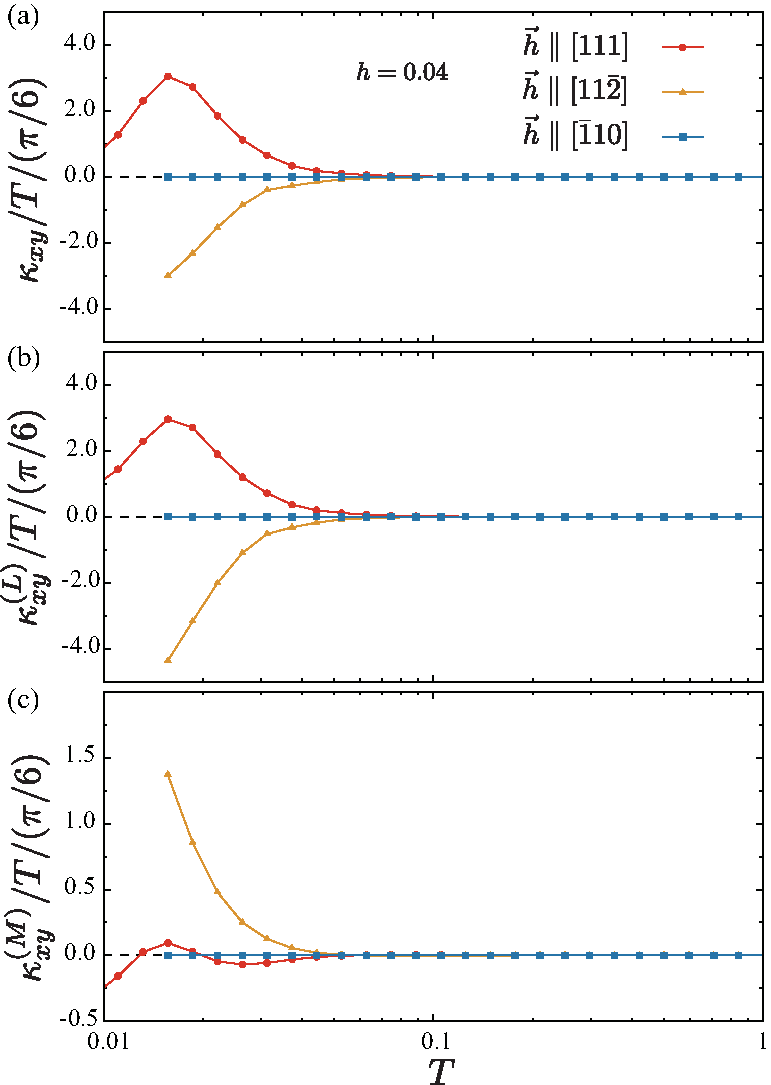
\includegraphics[width=0.9\linewidth]{Figs/plot_k_all_h0.04_ab.pdf}
%   \end{center}
%   \caption{{\bf \orange{Fig.6と7はmerge予定}}(a) Temperature dependence of $\kappa_{xy}/T$ of the ferromagnetic Kitaev model under magnetic fields parallel to $[111]$, $[11\bar{2}]$, and $[\bar{1}10]$ with $|h|=0.04$. The horizontal dashed line indicates $\kappa_{xy}/T = 0$. (b),(c) Contributions from the three-body ($L$) and the two-body ($M$) terms, respectively.}
%   \label{fig:k_all_h0.04_ab}
% \end{figure}

% \begin{figure}
%   \begin{center}
%     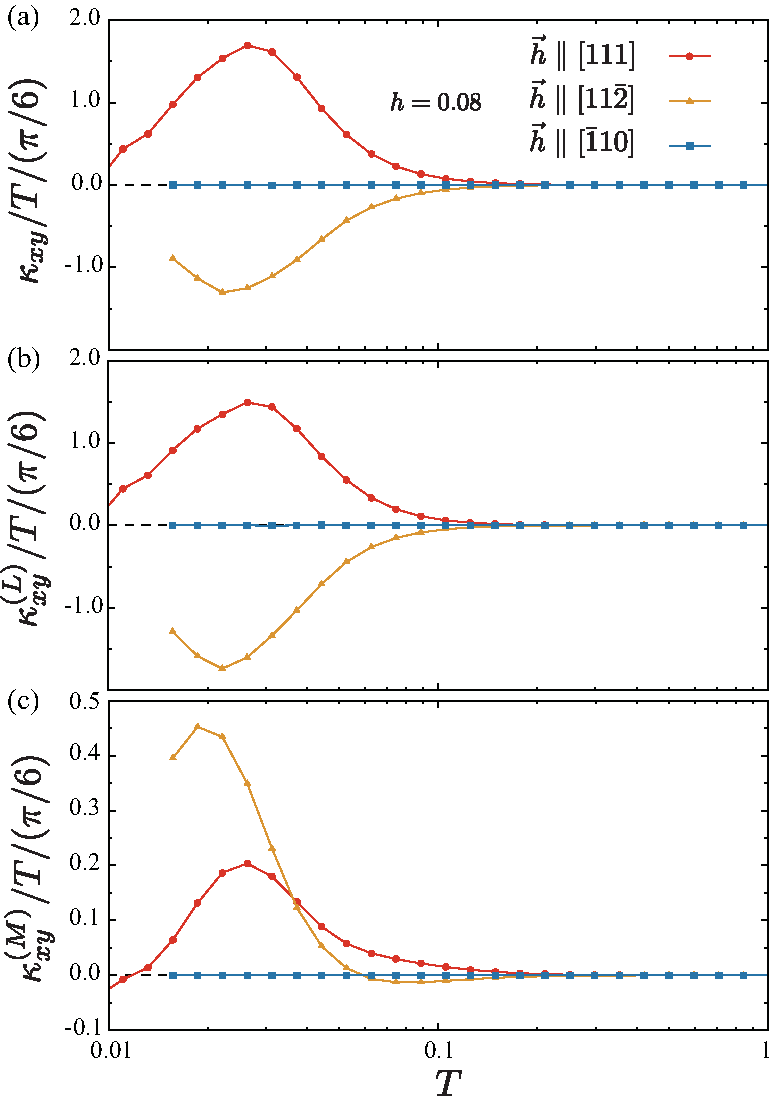
\includegraphics[width=0.9\linewidth]{Figs/plot_k_all_h0.08_ab.pdf}
%   \end{center}
%   \caption{(top) Temperature dependence of $\kappa_{xy}/T$ of the ferromagnetic Kitaev model under magnetic fields parallel to $[111]$, $[11\bar{2}]$, and $[\bar{1}10]$ with $|h|=0.08$. The horizontal dashed line indicates $\kappa_{xy}/T = 0$. The middle and bottom figures are contributions from the three-body ($L$) and the two-body ($M$) terms, respectively.}
%   \label{fig:k_all_h0.08_ab}
% \end{figure}
  
\subsection{Effect of non-Kitaev interactions}
\label{sec:Gamma}
%As we discussed above, the thermal Hall conductivity of the pure Kitaev model shows a peak at a finite temperature, and its value largely overshoots the half-quantized value. Here, 
In this subsection, we investigate the effects of the symmetric off-diagonal interactions, the $\Gamma$ and $\Gamma'$ terms, on the thermal Hall conductivity.
%From 
Based on the magnetic field dependence in the Kitaev model, the elementary excitations appear to be dominated by Majorana fermions rather than magnons, particularly %for 
in the weak magnetic field limit.
As we %denoted 
mentioned in Introduction, %from the 
according to the perturbative theory in the Majorana fermion representation, it is shown that
the negative $\Gamma^{\prime}$ enhances the Majorana gap~\cite{Takikawa_PRB2020}. %Hence, 
Therefore, %it is expected that
the thermal Hall conductivity is 
expected to be
enhanced by the negative $\Gamma^{\prime}$.
In contrast to $\Gamma^{\prime}$, the perturbative expansion with respect to $\Gamma$
is not straightforward, and it %is not at all clear 
remains unclear how $\Gamma$ affects the thermal Hall conductivity.
Here, we examine the %impacts 
impact of the $\Gamma'$ and $\Gamma$ %interactions 
terms in the original spin representation without assuming the Majorana excitations.

\subsubsection{Symmetric off-diagonal interaction $\Gamma^{\prime}$}
%{\bf\orange{[最初にわかりやすい摂動論の結果がある$\Gamma^{\prime}$を述べたほうがわかりやすい気がしたので、順番を入れ替えました。]}}
First, we consider the effect of the $\Gamma'$ interaction 
%to 
on $\kappa_{xy}/T$ %using 
under two representative magnetic fields %in 
along the [111] direction, 
$h=0.04$ and $h=0.08$. In Figs.~\ref{fig:all_h0.04_Gp}(a)--\ref{fig:all_h0.04_Gp}(c), 
we show several physical quantities for $-0.02\leq\Gamma'\leq0.02$. 
Here, we set %, here, 
$\Gamma = 0$ to only examine the %pure 
effects of $\Gamma'$ term. 
%Compared with $\Gamma$ terms, 
We find that $\Gamma^{\prime}$ does not significantly change 
the overall temperature dependence of the specific heat, %heights 
%are almost unchnaged by $\Gamma'$, 
%while 
although low-temperature peaks %slightly move 
shift slightly to higher (lower) temperatures %or lower temperatures 
for negative (positive) %and positive 
$\Gamma'$. %respectively. 
%Similar to the case of $\Gamma$ term, we see systematic change of the magnetization, although the observed changes are smaller than those in the case of $\Gamma$ (Fig.~\ref{fig:CMF_h0.04_ab} and \ref{fig:CMF_h0.04_ab}). Different from the $\Gamma$ term, the flux is almost unchanged by $\Gamma'$. 
We also find that the magnetization increases (decreases) monotonically for the negative (positive) $\Gamma'$.
In perturbation theory for the $\Gamma^{\prime}$ term~\cite{Takikawa_PRB2020}, it is shown that the gap is proportional to $-\Gamma^{\prime}/|K|$. This result
indicates that the effective magnetic field increases (decreases)
for the negative (positive)  $\Gamma^{\prime}$.
Therefore, the observed  $\Gamma'$ dependence of the magnetization 
is consistent with perturbation theory.
% \blue{[これは要確認]} \red{[これは、gap大とmagnetization大を対応させた議論なのかなと思いましたが、確かに、根拠がよく分からないですね...]}\orange{\bf 追記しました} \red{\textbf{$\to$ 確認しました}}.
In contrast to the magnetization, 
the flux does not show considerable changes as a function of $\Gamma^{\prime}$.

\begin{figure}
  \begin{center}
    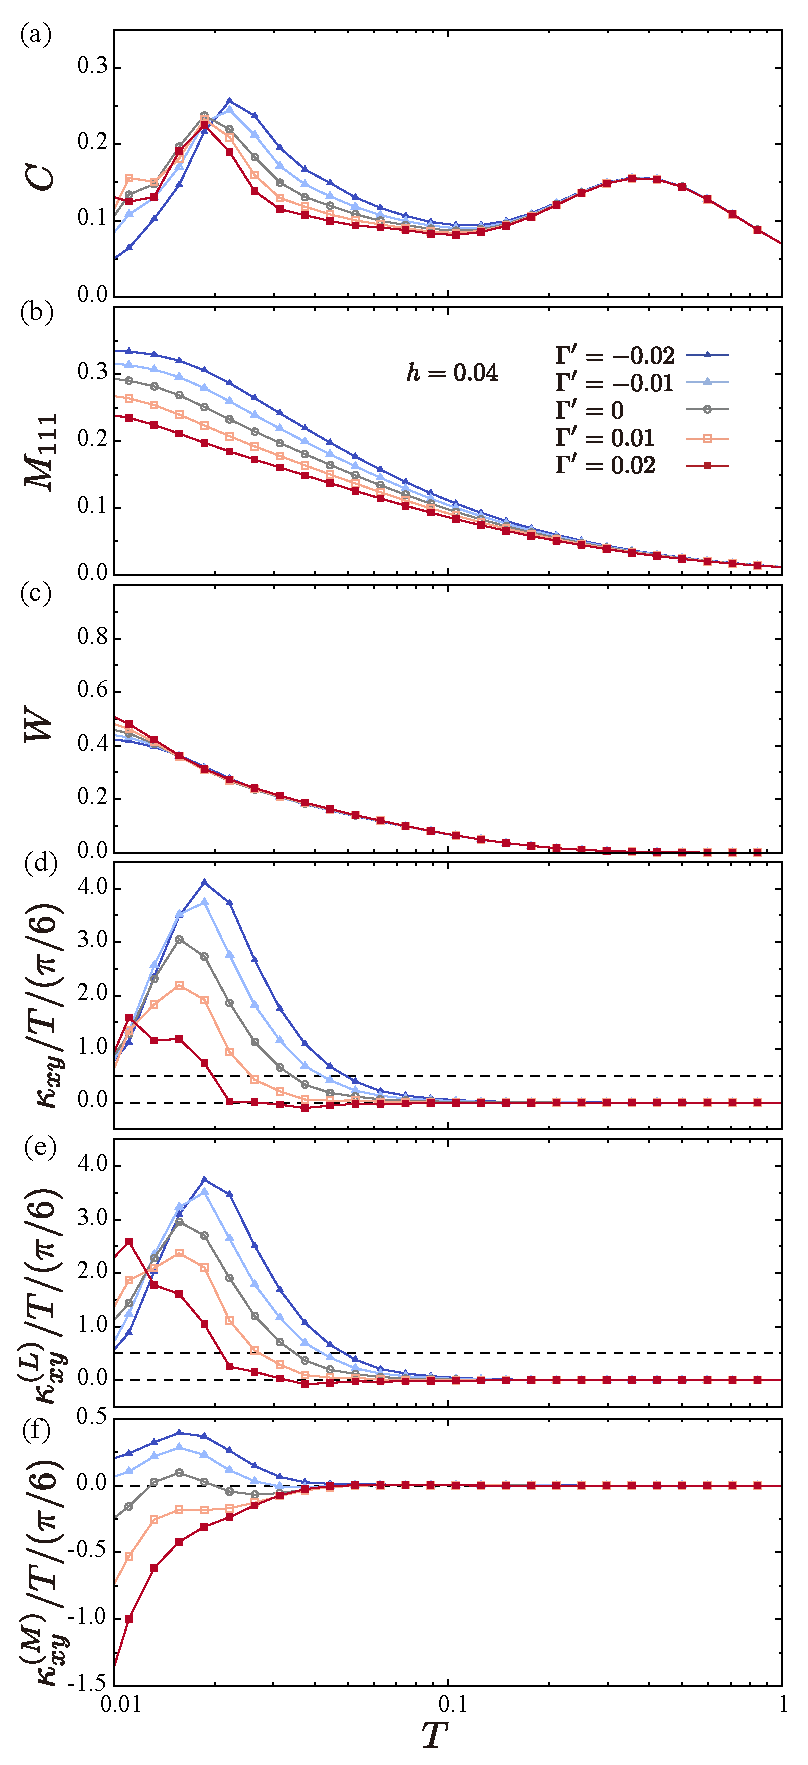
\includegraphics[width=0.9\linewidth]{Figs/plot_all_h0.04_Gp.pdf}
  \end{center}
  \caption{Temperature dependence of (a) the specific heat (b) the magnetic moment, (c) the flux 
   (d) the total thermal Hall conductivity $\kappa_{xy}/T$, 
   (e) the  three-body part of  the thermal Hall conductivity $\kappa_{xy}^{(L)}/T$, and 
   (f) the  two-body part of  the thermal Hall conductivity $\kappa_{xy}^{(M)}/T$ of the
  %ferromagnetic Kitaev model with a weak $\Gamma'$ u
  extended Kitaev model with $\Gamma=0$ and varying $\Gamma^{\prime}$
  under a magnetic field parallel to $[111]$ direction. The amplitude of the magnetic field is $|h|=0.04$.
  %\blue{[もう少し縦幅が狭い方がよい?]}\red{$\to$対応しました}
  }
  \label{fig:all_h0.04_Gp}
\end{figure}

\begin{figure}
  \begin{center}
    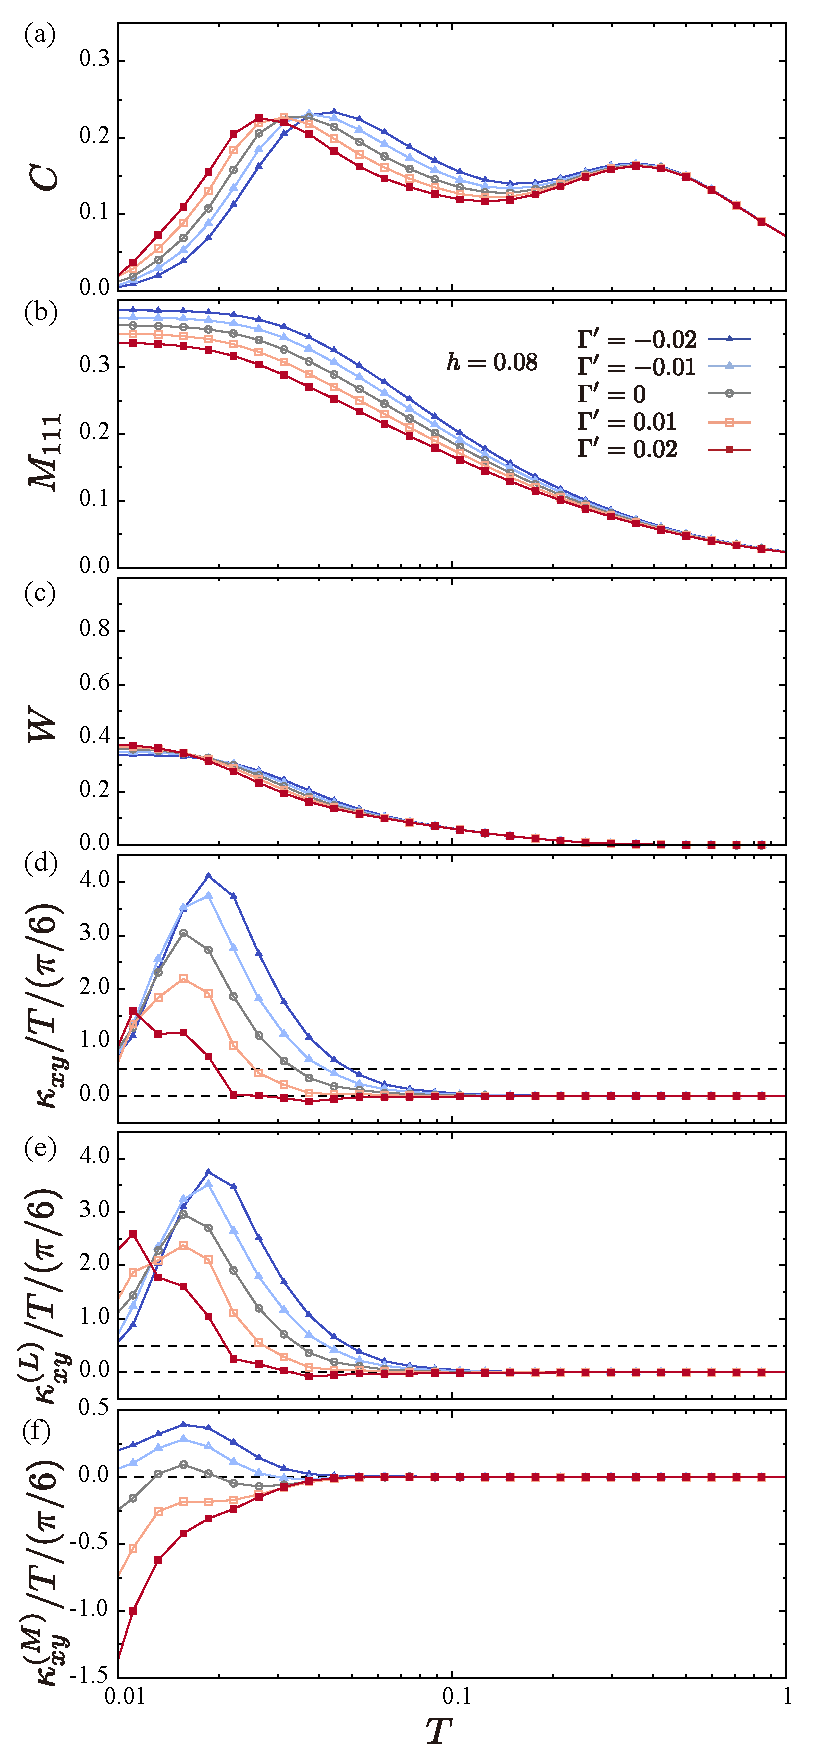
\includegraphics[width=0.9\linewidth]{Figs/plot_all_h0.08_Gp.pdf}
  \end{center}
  \caption{
     Corresponding plots to Fig.~\ref{fig:all_h0.04_Gp} for the extended Kitaev model with $\Gamma=0$, $h=0.08$ and varying $\Gamma^{\prime}$.
  %Temperature dependence of (a) the specific heat (b) the magnetic moment, and (c) the flux of the ferromagnetic Kitaev model with a weak $\Gamma'$ under a magnetic field parallel to $[111]$ direction. The amplitude of the magnetic field is $|h|=0.08$.
  %(d) Temperature dependence of $\kappa_{xy}/T$ of the ferromagnetic Kitaev model with as weak $\Gamma'$ interaction under a magnetic field parallel to $[111]$. The amplitude of the magnetic field is set to $|h|=0.08$. Two horizontal dashed lines indicate $\kappa_{xy}/T = 0$ and the half-quantized value. (e, f) Contributions from the three-body ($L$) and the two-body ($M$) terms, respectively.
  %\blue{[もう少し縦幅が狭い方がよい?]}\red{$\to$対応しました}
  }
  \label{fig:all_h0.08_Gp}
\end{figure}

Figs.~\ref{fig:all_h0.04_Gp}(d)--\ref{fig:all_h0.04_Gp}(f) show the temperature dependence of $\kappa_{xy}/T$ %with 
for the same values of $\Gamma'$. Although the effects %\red{to} 
on the %usual 
bulk physical quantities are small as we have shown above, 
$\Gamma^{\prime}$ %largely 
significantly changes $\kappa_{xy}/T$; when we decrease %$\Gamma'$ 
$\Gamma'$ from $0.02$, the peak of $\kappa_{xy}/T$ %moves 
shifts to higher temperature %with increasing its height.
while its height increases.
In particular, for the negative (positive) $\Gamma'$, 
an
%the 
increase of its absolute value %leads to the 
results in an enhancement (suppression) of $\kappa_{xy}/T$.
% , while the peak moves to lower temperature with decreasing its height for positive \red{$\Gamma'$}.
Such sign-dependent changes %of 
in $\kappa_{xy}$ are %somewhat 
broadly consistent with the 
results from perturbation theory \cite{TakikawaF2020}. 

We also find that $\Gamma^{\prime}$ monotonically %decreases 
reduces both the three-body part and the two-body part of $\kappa_{xy}$;
With increasing %$\Gamma^{\prime}$ 
from $\Gamma'=-0.02$, $\kappa_{xy}^{(L)}$ is suppressed and its peak shifts 
%to the 
toward lower temperatures %low-temperature side
[Fig.~\ref{fig:all_h0.04_Gp}(e)], similar to the total thermal Hall conductivity [Fig.~\ref{fig:all_h0.04_Gp}(d)].
On the other hand, $\kappa_{xy}^{(M)}$ exhibits %the 
a sign change from %the 
positive to negative [Fig.~\ref{fig:all_h0.04_Gp}(f)]. 
For $\Gamma^{\prime}\geq0.01$, 
%the two-body part $\kappa_{x}^{(M)}$ becomes negative and 
there is a competition between the positive $\kappa_{xy}^{(L)}$ and the negative $\kappa_{xy}^{(M)}$.
As a result, %in 
at $\Gamma^{\prime} = 0.02$ and $h=0.04$, %$h=0.05$, 
the total $\kappa_{xy}/T$ %becomes 
turns negative around $T=0.04$, 
although its absolute value is small. 
%\orange{このnegativeになる記述は必要?}$\to$ \red{残したいです}
%\orange{では、残しましょう}
%Note that correspondence between the peak temperature and the height is different from that for the $\Gamma$ (See Figs.~\ref{fig:k_all_h0.04_G}(a) and \ref{fig:k_all_h0.08_G}(a)).
%In the case of negative $\Gamma$ we observed that the peak moves higher temperature \textit{with decreasing its height}. Such qualitative difference might be useful to compare the present model calculation to experimental observations. 

%{\bf\orange{ここはとりあえず残しています}}\blue{[カット予定?]}
%Another important feature is negative $\kappa_{xy}/T$ observed at $\Gamma' = 0.02$ with $h = 0.04$. Although it is relatively small, we observe negative values both in $\kappa_{xy}^{(L)}/T$ and $\kappa_{xy}^{(M)}/T$. \textcolor{red}{In addition, we will see similar negative $\kappa_{xy}/T$ in the classical model (Need to check the classical counterpart)}\blue{$\to$ Classicalの場合は、$\Gamma'$の方でのみ負になっています。古典系の部分では、$\Gamma'$導入の場合より$\Gamma$の方が量子性が効いていているのでは?という感じで書いていますが、ご検討お願いします}. Thus, we conclude that positive $\Gamma'$ can change the sign of $\kappa_{xy}/T$.


\subsubsection{Symmetric off-diagonal interaction $\Gamma$} 
Next, we investigate the effects of the 
$\Gamma$ term on $\kappa_{xy}/T$ under a magnetic field parallel to the $[111]$ direction. 
Again, we consider two representative magnetic fields, $h=0.04$ and $h=0.08$.
In Figs.~\ref{fig:all_h0.04_G}(a)--\ref{fig:all_h0.04_G}(c), we show the temperature dependence 
of the specific heat, the magnetization, and the flux for $-0.02\leq\Gamma\leq0.02$. Although the %amplitudes 
magnitudes of $\Gamma$ are relatively small, 
we find that the low-temperature peaks of the specific heat show 
significant change. %in the low-temperature peaks in the specific heat. 
For negative $\Gamma$, the peak %moves 
shifts to a higher temperature, with an increase in its height.
%and its height is enhanced. 
Similarly, the magnetization increases for negative $\Gamma$. 
%In the case of 
For positive $\Gamma$, we observe the opposite effects.
%, so that, the low-temperature peak of the specific heat moves lower temperature with decreasing its height, and magnetizations decreases. 
%Both negative and positive $\Gamma$s almost do not affect the 
%the high-temperature peak of the specific heat. 
We can also see sign-dependent changes in the flux around the intermediate temperature region $T\sim0.03$, 
although %it 
the effect is not so significant. 
% in the case of $h=0.04$ with positive $\Gamma$. 

\begin{figure}
  \begin{center}
    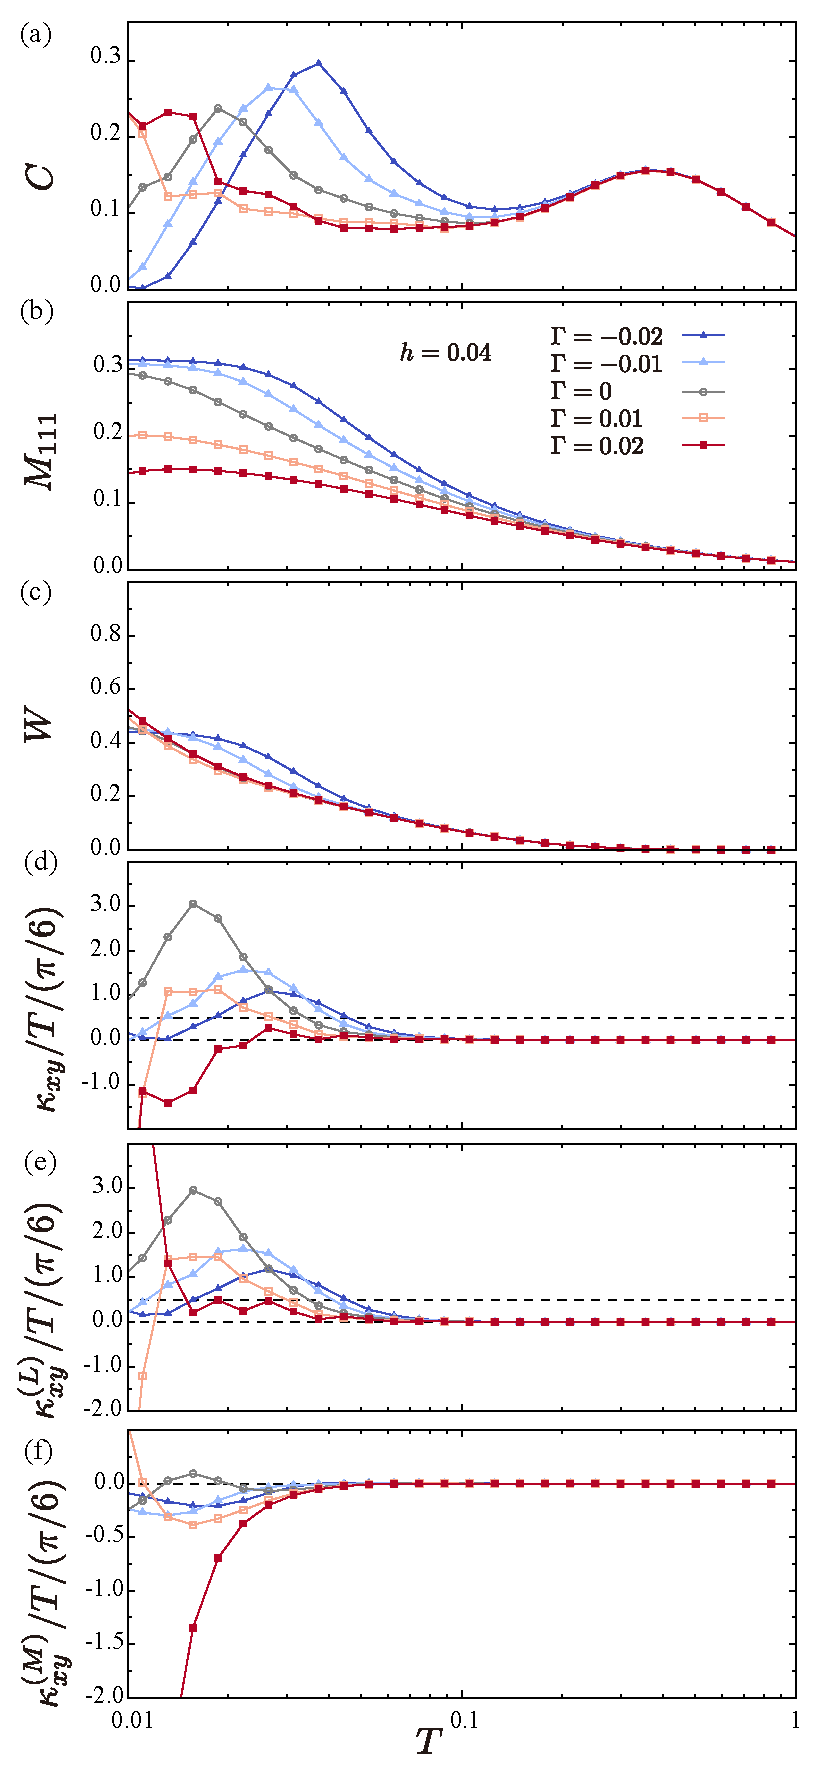
\includegraphics[width=0.9\linewidth]{Figs/plot_all_h0.04_G.pdf}
  \end{center}
  \caption{
 Corresponding plots to Fig.~\ref{fig:all_h0.04_Gp} for the extended Kitaev model with $\Gamma^{\prime}=0$, $h=0.04$ and varying $\Gamma$. 
  %Temperature dependence of (a) the specific heat (b) the magnetic moment, and (c) the flux of the ferromagnetic Kitaev model with a weak $\Gamma$ under a magnetic field parallel to $[111]$ direction. The amplitude of the magnetic field is $|h|=0.04$.
  %(d) Temperature dependence of $\kappa_{xy}/T$ of the ferromagnetic Kitaev model with as weak $\Gamma$ interaction under a magnetic field parallel to $[111]$. The amplitude of the magnetic field is set to $|h|=0.04$. Two horizontal dashed lines indicate $\kappa_{xy}/T = 0$ and the half-quantized value. (e, f) Contributions from the three-body ($L$) and the two-body ($M$) terms, respectively. The insets show magnified views for $\Gamma = 0.02$.
  %\blue{[もう少し縦幅が狭い方がよい?]}\red{$\to$対応しました}
  }
  \label{fig:all_h0.04_G}
\end{figure}
\begin{figure}
  \begin{center}
    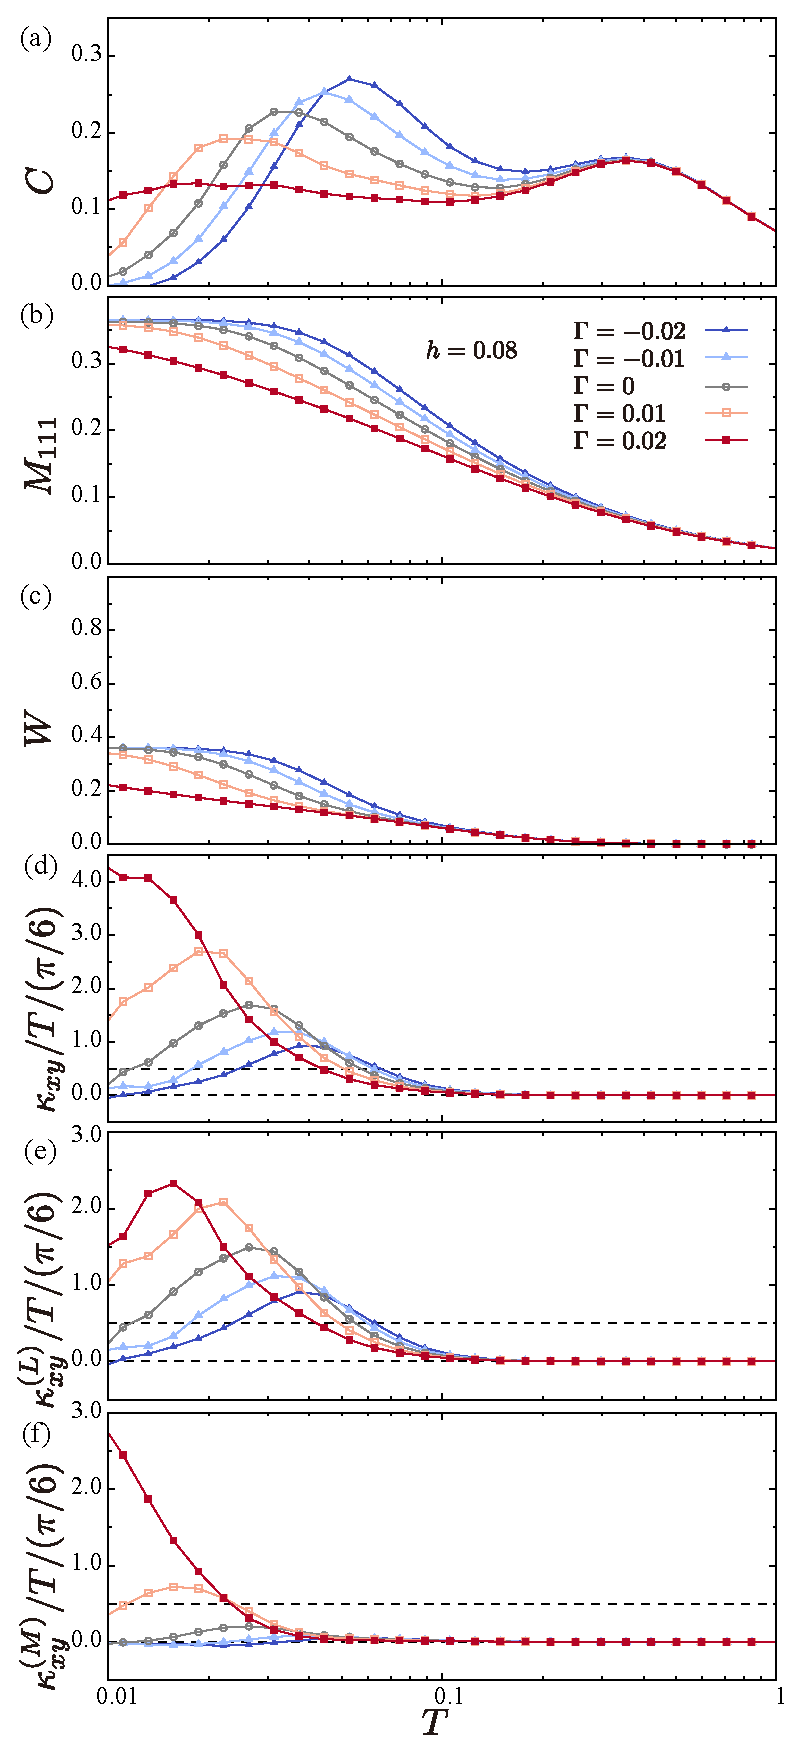
\includegraphics[width=0.9\linewidth]{Figs/plot_all_h0.08_G.pdf}
  \end{center}
  \caption{
   Corresponding plots to Fig.~\ref{fig:all_h0.04_Gp} for the extended Kitaev model with $\Gamma^{\prime}=0$, $h=0.08$ and varying $\Gamma$. 
  %Temperature dependence of (a) the specific heat (b) the magnetic moment, and (c) the flux of the ferromagnetic Kitaev model with a weak $\Gamma$ under a magnetic field parallel to $[111]$ direction. The amplitude of the magnetic field is $|h|=0.08$.
  %(d) Temperature dependence of $\kappa_{xy}/T$ of the ferromagnetic Kitaev model with as weak $\Gamma$ interaction under a magnetic field parallel to $[111]$. The amplitude of the magnetic field is set to $|h|=0.08$. Two horizontal dashed lines indicate $\kappa_{xy}/T = 0$ and the half-quantized value. (e, f) Contributions from the three-body ($L$) and the two-body ($M$) terms, respectively.
  %\blue{[もう少し縦幅が狭い方がよい?]}\red{$\to$対応しました}
  }
  \label{fig:all_h0.08_G}
\end{figure}

%When we see $\kappa_{xy}/T$ 
As shown in Figs.~\ref{fig:all_h0.04_G}(d)--\ref{fig:all_h0.04_G}(f), 
we find that the $\Gamma$ %interaction 
term %can change 
has a significant impact on the thermal Hall conductivity. %significantly.
Negative $\Gamma$ suppresses $\kappa_{xy}/T$ for both %for 
$h = 0.04$ and $h=0.08$. 
%In the case of 
For positive $\Gamma$, we %see 
observe different behaviors between $h = 0.04$ and $h=0.08$. For $h=0.04$, positive $\Gamma$ %largely 
strongly suppresses $\kappa_{xy}/T$, and it becomes even negative for $\Gamma = 0.02$. In contrast to $h=0.04$, we %see
observe that positive $\Gamma$ enhances $\kappa_{xy}/T$. Such %huge 
large changes in $\kappa_{xy}/T$ by small $\Gamma$ seem to be different from the result of perturbation theory, %; it shows the contributions from $\Gamma$ appear as the 
where contributions from $\Gamma$ appear only at third order~\cite{YamadaF2021}. 

This magnetic field-dependent behavior might be related to the large magnitude of $\kappa_{xy}^{(M)}/T$ observed for positive $\Gamma$. For $\Gamma \le 0$, $\kappa_{xy}^{(L)}$ dominates the total $\kappa_{xy}/T$.
However, for $\Gamma = 0.01$ and $0.02$ at $h=0.04$, %the amplitudes of $\kappa_{xy}^{(M)}/T$ become larger, in particular for $\Gamma = 0.02$.
the low-temperature value of $\kappa_{xy}^{(M)}/T$ %largely
significantly changes as shown in Fig.~\ref{fig:all_h0.04_G}(f).%\blue{[$\Gamma=0.02$から0.01の方向なのかわからなかったので、changes の方が良いでしょうか?もしくは、with decreasing $\Gamma$などを加えるとかでしょうか。]} \red{[$\to$ おっしゃる通りです。changesにしました。]}
This abrupt change may %recall 
indicate the presence of a phase transition from the Kitaev QSL to another phase, such as a spin nematic state, %which is 
as suggested by %using the 
infinite tensor network calculations at zero temperature~\cite{Lee_NCom2020}.
% This enhancement of the contribution from the two-body correlation might be related to nematic phases
% at the zero temperature observed in the infinite tensor network calculation~\cite{Lee_NCom2020}.
%{\bf[\orange{nematic だと2体項が大きくなる理由はある?}]}
%\blue{[少し表現を変えて、相転移を示唆するくらいにしてみました]}
   
%\clearpage
 \subsection{Classical limit}
\label{sec:classicalMC}

In this section, we show the results obtained by applying the classical approximation %for 
to Eq.~\eqref{eq:model-Hamiltonian} to compare %those 
them with those of %for 
the quantum spin model shown above.
First, we focus on the pure Kitaev model with $\Gamma=\Gamma'=0$.
Figure~\ref{fig_classical_hdep}(a) shows the temperature dependence of the specific heat of the classical Kitaev model at several magnetic fields along the $[111]$ direction.
In the absence of the magnetic field, %the 
previous studies %clarified 
have shown that the specific heat monotonically increases with decreasing temperature and approaches $3/4$ in the zero temperature limit~\cite{Sela2014,Suzuki2018_2}.
This value originates from the zero modes that are intrinsic to the pure Kitaev model without a magnetic field, and the quartic order of the spin fluctuations contributes to the specific heat at $T\to 0$.
Once the magnetic field is introduced, it lifts the zero modes, and thereby, the zero-$T$ limit of the specific heat takes the conventional value, i.e., 1, owing to the presence of the two continuous variables $(\theta,\phi)$ at each site.
We find that it shows a shoulder-like structure %a peak \orange{[peakがある?shoulder程度?]}
at the temperature corresponding to the energy scale of $h$ in the presence of the magnetic field despite the monotonic change at $h=0$.
In this temperature scale, the magnetization monotonically increases as a function of the magnetic field,
%develops, 
as shown in Fig.~\ref{fig_classical_hdep}(b).

\begin{figure}[tbh] 
\begin{center} 
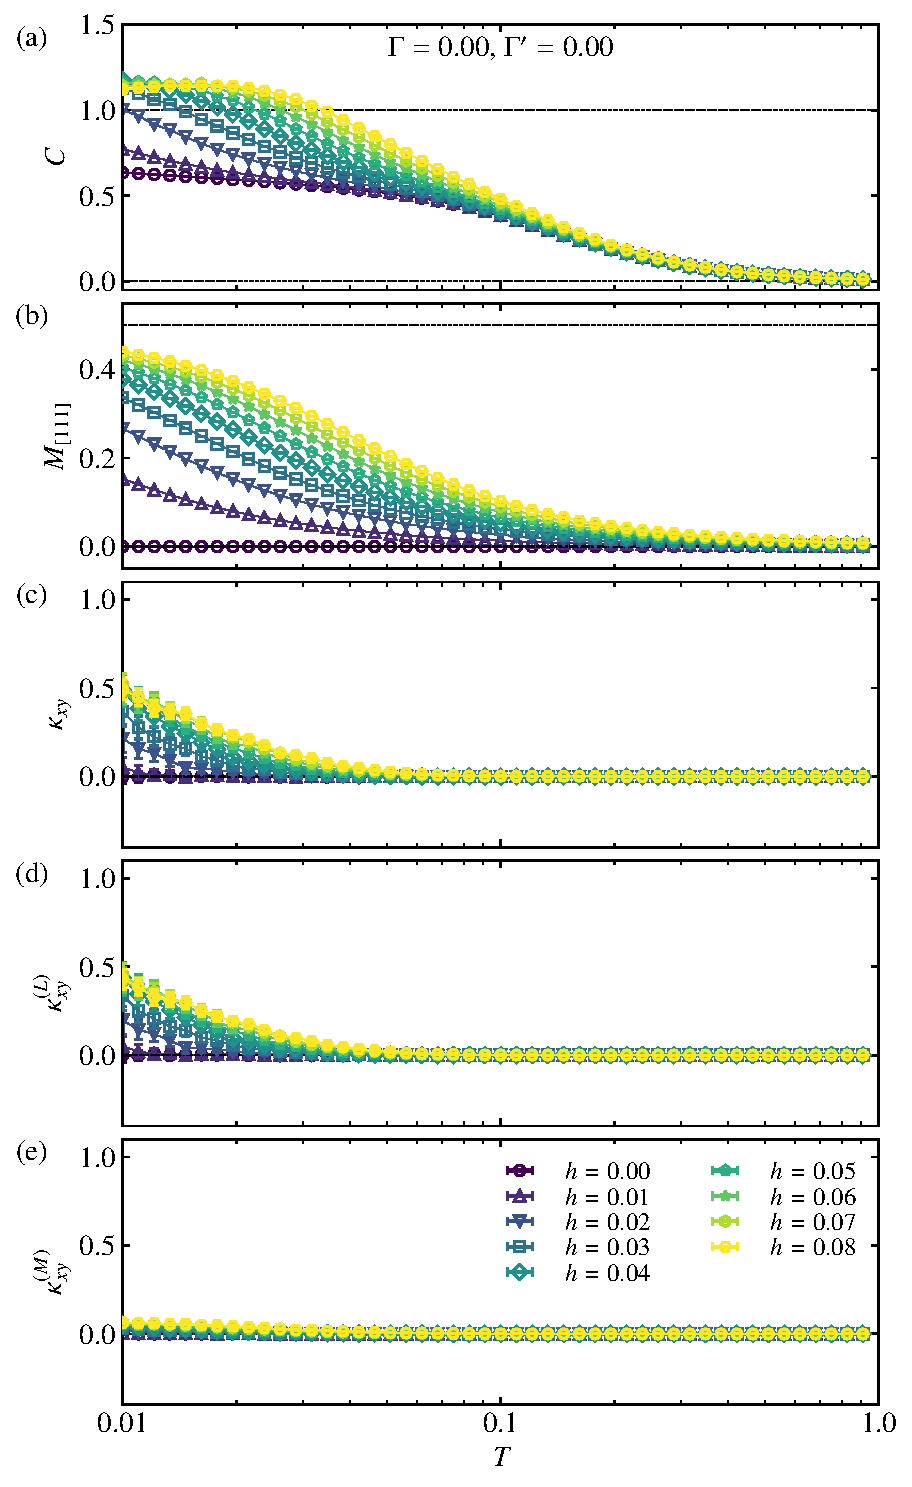
\includegraphics[width=0.9\linewidth]{Figs/fig_K-1.0_G0.00_Gp0.00_c.pdf}
\vspace{-0.5cm} 
\caption{Temperature dependence of (a) the specific heat, (b) the total magnetization, and
(c) the thermal Hall conductivity $\kappa_{xy}$ for several magnetic fields along the $[111]$ direction in the classical Kitaev model.
(d),(e) Temperature dependence of the two components, $(L)$ and $(M)$, of the thermal Hall conductivity.}
\label{fig_classical_hdep}
\end{center}
\end{figure}


Figure~\ref{fig_classical_hdep}(c) shows the thermal Hall conductivity $\kappa_{xy}$ as a function of temperature.
When the magnetic field is not applied, 
$\kappa_{xy}$ is always zero.
By introducing the magnetic field, $\kappa_{xy}$ becomes nonzero and positive, which is consistent with the results for the quantum system.
Moreover, the temperature scale %for developing 
at which the thermal Hall conductivity 
develops
is much smaller than that for the magnetization.
The distinctly different temperature scales %appear to be 
are similar to those in the quantum system [see Fig.~\ref{fig:CMF_pure}] although the double-peak structure of the specific heat is not observed in the classical system.
In the classical result, $\kappa_{xy}$ shows a monotonic increase with decreasing temperature.
On the other hand, in the quantum system, $\kappa^{xy}/T$ %takes 
exhibits a peak around the temperature at which the specific heat exhibits the low-$T$ peak, as shown in Fig.~\ref{fig:CMF_pure}(d). %(e).
The difference is considered to originate from an artifact in the classical system, where the macroscopic degeneracy is present in the low-energy region.
The degeneracy also causes the nonzero specific heat at zero temperature. %leading to the nonzero specific heat at zero temperature.
Thus, the quantization of $\kappa^{xy}/T$ does not occur in the classical system.
Figures~\ref{fig_classical_hdep}(d) and \ref{fig_classical_hdep}(e) present the three-body and two-body contributions of the thermal current to the thermal Hall conductivity, respectively.
The two-body %contributions 
contribution $\kappa_{xy}^{(M)}$ is much smaller than the three-body one $\kappa_{xy}^{(L)}$, indicating that the thermal Hall effect is dominated by the three-body terms of the thermal current at the edges.
This result is consistent with the quantum system, but the classical approximation appears not to reproduce small negative values of $\kappa_{xy}^{(M)}$ in weak magnetic fields as shown in Fig.~\ref{fig:CMF_pure}(f). %Thus, this
The difference suggests that the negative $\kappa_{xy}^{(M)}$ may be induced by
quantum effects.

\begin{figure}[tbh] 
\begin{center} 
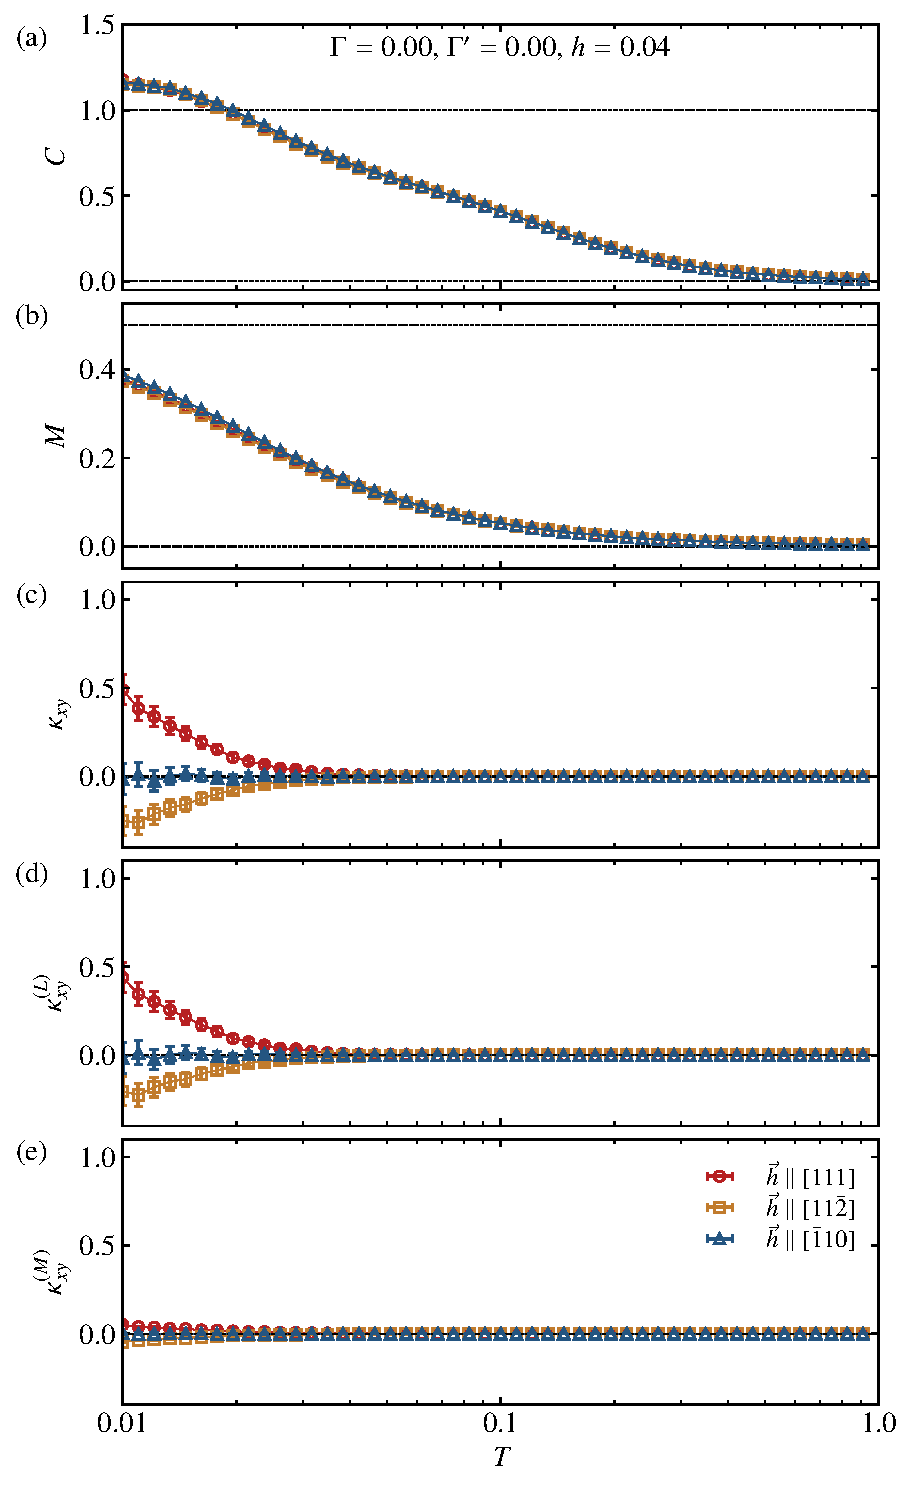
\includegraphics[width=0.9\linewidth]{Figs/fig_K-1.0_G0.00_Gp0.00_h0.04.pdf}
\vspace{-0.5cm} 
\caption{Temperature dependence of (a) the specific heat, (b) the total magnetization, and
(c) the thermal Hall conductivity $\kappa_{xy}$ in the classical Kitaev model under the magnetic field parallel to $[111]$, $[11\bar{2}]$, and $[\bar{1}10]$ with $h=0.04$.
(d),(e) Temperature dependence of the two components, $(L)$ and $(M)$, of the thermal Hall conductivity.}
\label{fig_classical_adep004}
\end{center}
\end{figure}
  
Next, we discuss the field-angle dependence of physical quantities in the pure Kitaev model. We consider %the 
three field directions $[11\bar{2}]$, $[\bar{1}10]$, and $[111]$, which are perpendicular to each other.
Figures~\ref{fig_classical_adep004}(a) and \ref{fig_classical_adep004}(b) show the temperature dependence of the specific heat and magnetization along the corresponding field %direction.
directions.
These results indicate that the field direction hardly changes the specific heat and magnetization, which is also observed in the quantum system (see Fig.~\ref{fig:CMF_ab}). 
% \blue{[図がないので大久保さんの方で確認お願いします]}\red{(実は、appendixに置いてありました。最終的にどうするかわからないですが、とりあえずその図を参照。)}.
%On the other hand, 

In contrast to these bulk physical quantities, the thermal Hall conductivity strongly depends on the direction of the applied magnetic field.
As shown in Fig.~\ref{fig_classical_adep004}(c), $\kappa_{xy}$ is negative and decreases with decreasing temperature for $\vec{h}\parallel [11\bar{2}]$, 
%in contrast to the case with 
whereas it is positive for
$\vec{h}\parallel [111]$.
Moreover, the absolute value for the former is smaller than that for the latter.
While %these %characteristics 
the overall %behaviors are 
behavior is consistent with that %in 
of the quantum system, the peak structure in Fig.~\ref{fig:CMF_ab}(d) is not seen in the classical case.
Furthermore, a large enhancement of $\kappa_{xy}^{(M)}$ at low temperatures for $\vec{h}\parallel [11\bar{2}]$ presented in Fig.~\ref{fig:CMF_ab}(f) is not reproduced in the classical system as shown in Fig.~\ref{fig_classical_adep004}(e) despite the %similarity for the temperature 
similar temperature dependence of $\kappa_{xy}^{(L)}$ in the quantum and classical systems [Figs.~\ref{fig:CMF_ab}(e) and \ref{fig_classical_adep004}(d)].
This result suggests that the three-body term can be understood in the classical picture, but quantum fluctuations beyond the classical approach substantially contribute to the two-body term.
% \red{[2体項はtime-reversal evenで、磁場によって古典的に誘発されたものではないから??]}
% \red{[以下は、量子系のところに入れた方が良いかも]}
We also find that the thermal Hall conductivity is zero in the magnetic field applied along the $[\bar{1}10]$ direction, which is %results in 
a consequence of the symmetry of the Hamiltonian, as discussed before.
% This is understood from the fact that the Hamiltonian is invariant under the following two operations simultaneously:
% The $C_2$ rotation along the $[\bar{1}10]$ axis in the spin space transferring $(S^x,S^y,S^z)$ to $(-S^y,-S^x,-S^z)$ and the rotation of the honeycomb plane along the $z$~bond in the real space, which exchanges the $x$ and $y$~bonds.
% However, the rotation of the honeycomb plane inverts the component along the zigzag edge of the position vector $\bm{r}$, and thereby, the thermal current along the zigzag edge should be zero.
% Note that the above argument is applicable in the presence of the $\Gamma$ and $\Gamma'$ interactions.

% \begin{figure}[tbh] 
%   \begin{center} 
%   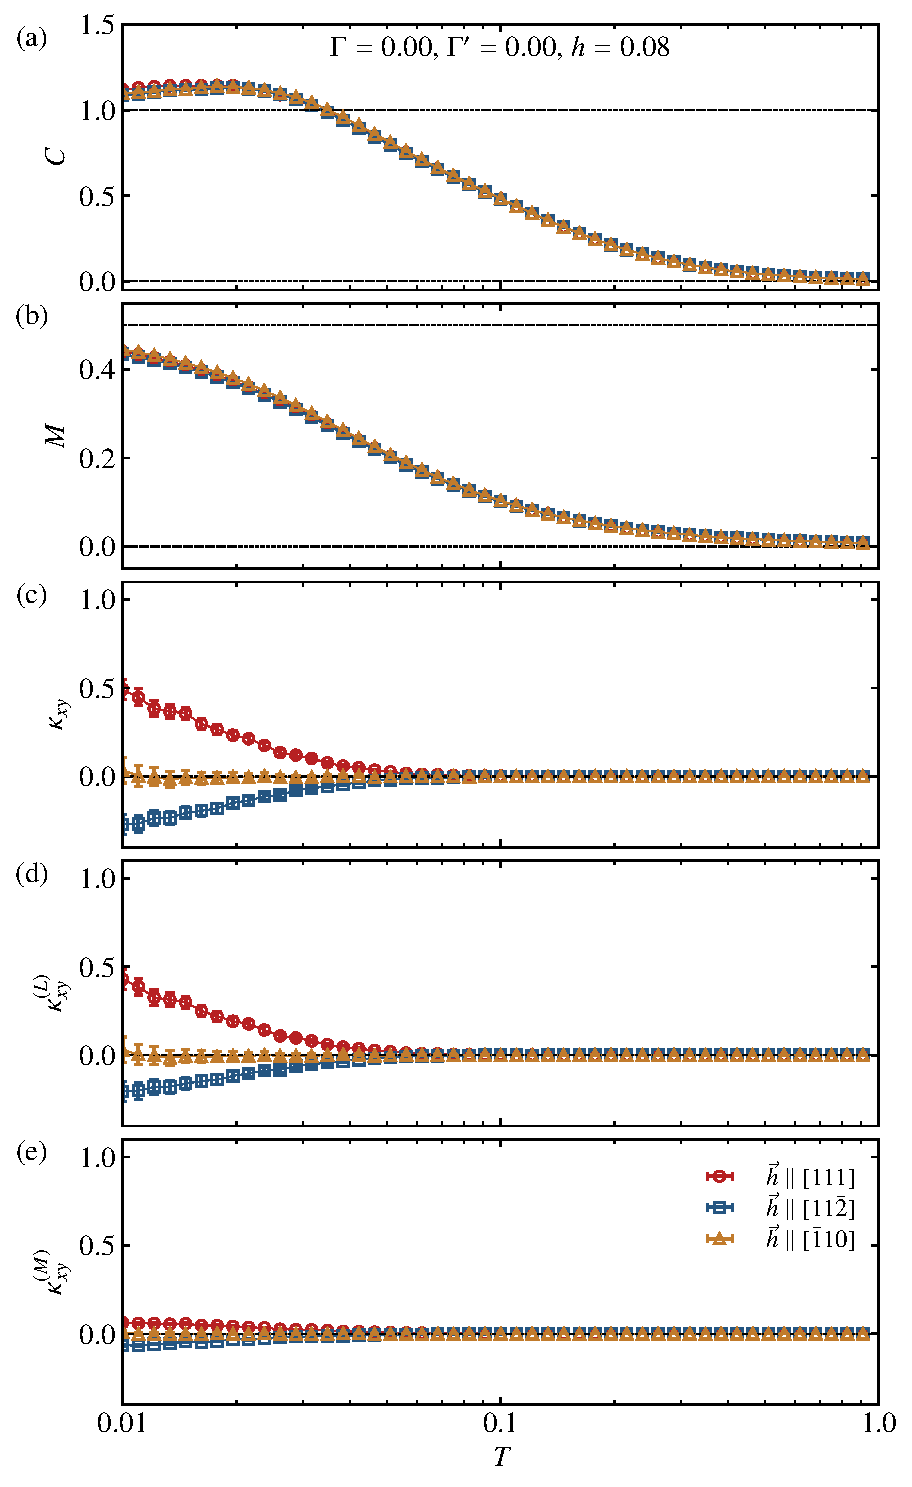
\includegraphics[width=0.9\linewidth]{fig_K-1.0_G0.00_Gp0.00_h0.08.pdf}
%   \vspace{-0.5cm} 
%   \caption{Temperature dependence of (a) the specific heat, (b) the total magnetization, and
%   (c) the thermal Hall conductivity $\kappa_{xy}$ in the classical Kitaev model under the magnetic field parallel to $[111]$, $[11\bar{2}]$, and $[\bar{1}10]$ with $h=0.08$.
%   (d),(e) Temperature dependence of the two components, $(L)$ and $(M)$, of the thermal Hall conductivity.}
%   \label{fig_classical_adep008}
%   \end{center}
%   \end{figure}


\begin{figure}[tbh] 
\begin{center} 
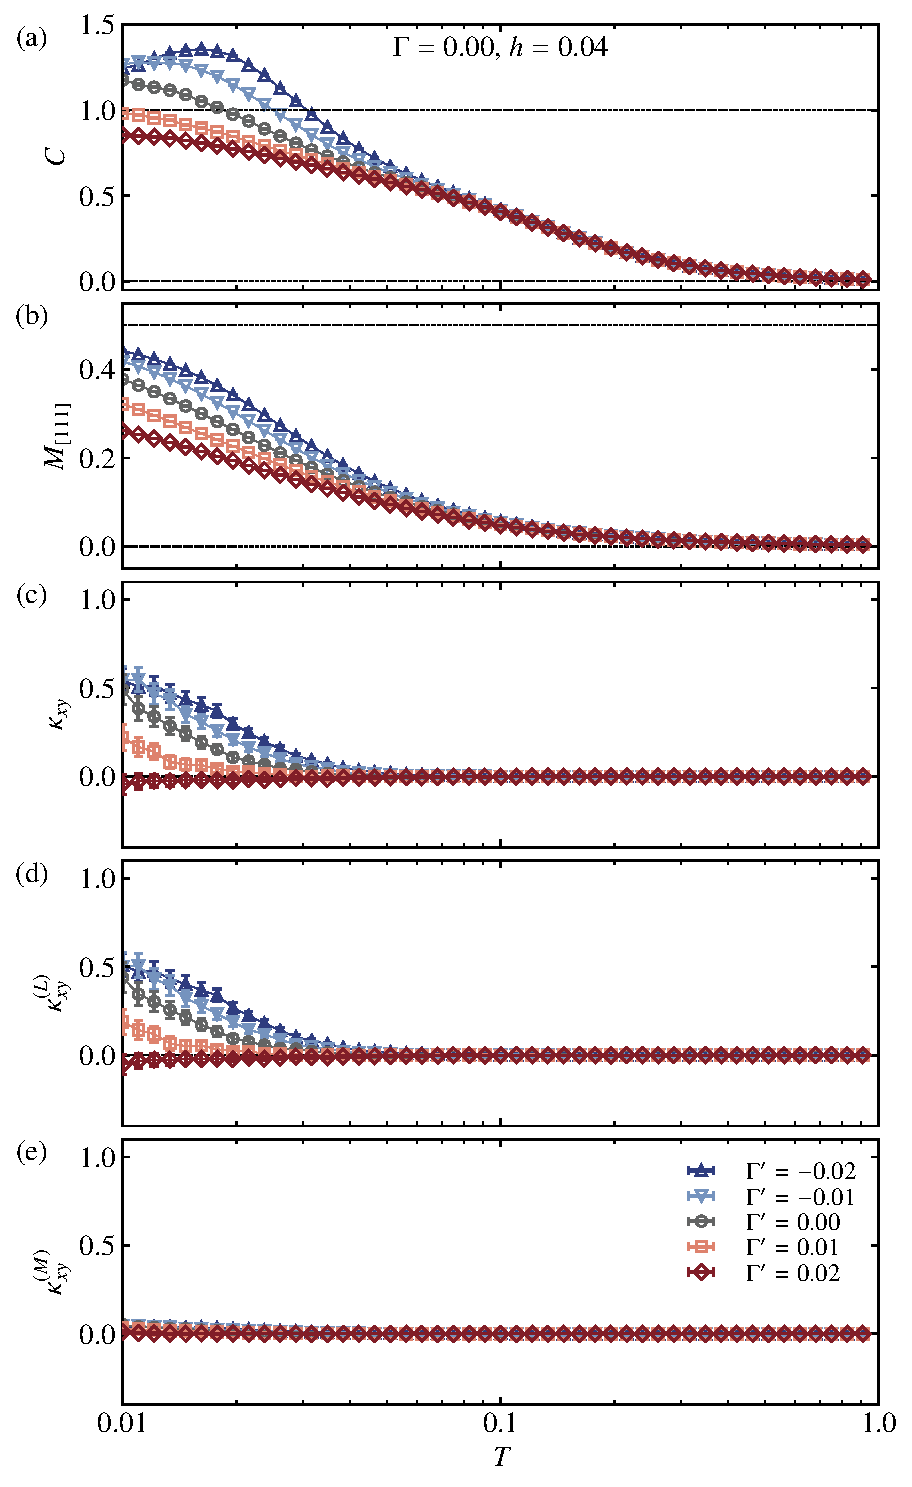
\includegraphics[width=0.9\linewidth]{Figs/fig_K-1.0_G0.00_h0.04.pdf}
\vspace{-0.5cm} 
\caption{Temperature dependence of (a) the specific heat, (b) the total magnetization, and
(c) the thermal Hall conductivity $\kappa_{xy}$ in the classical Kitaev-$\Gamma'$ model under the magnetic field with $h=0.04$.
(d),(e) Temperature dependence of the two components, $(L)$ and $(M)$, of the thermal Hall conductivity.}
\label{fig_classical_gpdep004}
\end{center}
\end{figure}

%\orange{[ここも量子系に合わせて$\Gamma^{\prime}$を最初に変更]}
Here, we introduce the $\Gamma'$ and $\Gamma$ interactions in the Kitaev model.
First, we examine the %effect 
effects of the $\Gamma'$ interaction on the Kitaev system.
Figure~\ref{fig_classical_gpdep004} shows the temperature dependence of physical quantities for several values of $\Gamma'$ %in the Kitaev-$\Gamma'$ model 
without the $\Gamma$ interaction.
%The 
A positive $\Gamma'$ suppresses the specific heat and magnetization, %while the 
whereas a negative $\Gamma'$ enhances them.
Moreover, we %find 
observe a peak in the specific heat at $\Gamma'=-0.02$ in Fig.~\ref{fig_classical_gpdep004}, indicating its shift to %the high-temperature side 
higher temperatures with decreasing $\Gamma'$.
These tendencies are also seen in the quantum system, as shown in Figs.~\ref{fig:all_h0.04_Gp}(a) and \ref{fig:all_h0.04_Gp}(b).

%For the thermal transport, 
Regarding thermal transport,
we find that the negative (positive) $\Gamma'$ enhances (suppresses) the thermal Hall conductivity [Fig.~\ref{fig_classical_gpdep004}(c)]. We note that $\kappa_{xy}$ becomes 
negative at low temperatures for $\Gamma'=0.02$.
We also find that
the three-body part %dominantly contributes 
is the dominant contribution to the thermal Hall conductivity, as shown in Figs.~\ref{fig_classical_gpdep004}(d) and \ref{fig_classical_gpdep004}(e).
Thus, the overall tendency is consistent with that of the quantum systems.
%Here, we compare the above results with those in the quantum system presented in Fig.~\ref{fig:all_h0.04_Gp}.
%As discussed \blue{before,} %in the previous paragraph for the $\Gamma$ dependence,
Furthermore, by examining the temperature dependence in detail, 
we find that
results for the classical limit %should be compared 
are %well consistent 
in good agreement with those for the intermediate temperature range ($T\sim 0.05$) in the quantum system, as
shown in Fig.~\ref{fig:all_h0.04_Gp}(d). %(a).
%Although the thermal Hall conductivity in this system takes a positive value at the lowest temperature [Fig.~\ref{fig:all_h0.04_Gp}(a)], 
In the quantum systems around $T=0.05$, 
$\kappa_{xy}$ 
%\red{[厳密には$\kappa_{xy}/T$な気がしましたが、修正するほどかどうか迷いました。]}
decrease monotonically by increasing $\Gamma^{\prime}$
and %it 
appears to be negative for $\Gamma^{\prime}=0.02$.
Moreover, in this temperature range, $\kappa_{xy}^{(M)}$ is much smaller than $\kappa_{xy}^{(L)}$, as shown in Figs.~\ref{fig:all_h0.04_Gp}(e) and \ref{fig:all_h0.04_Gp}(f).
%which are consistent with the corresponding results for the classical system.
These results indicate that $\kappa_{xy}$ in the classical systems corresponds to %that 
$\kappa_{xy}$ in the 
quantum systems at intermediate temperatures, where %the effects of the 
quantum fluctuations are expected to be small.

Finally, we %focus on 
examine the effect of the $\Gamma$ term.
Figure~\ref{fig_classical_gdep004} shows the temperature dependence of physical quantities %at
for several values of $\Gamma$, %with 
setting $\Gamma'=0$.
For %the case of the 
negative $\Gamma$, the low-$T$ specific heat is enhanced with increasing the absolute value of $\Gamma$, as shown in Fig.~\ref{fig_classical_gdep004}(a).
On the other hand, the specific heat is suppressed by %the introduction of the 
introducing a positive $\Gamma$.
These tendencies are consistent with the results in the quantum system, %while 
whereas the peak structure shown in Fig.~\ref{fig:all_h0.04_G}(a) is not reproduced in the classical simulations.
Figure~\ref{fig_classical_gdep004}(b) shows the temperature dependence of the magnetization %at
for several values of %several 
$\Gamma$.
The magnetization increases with decreasing $\Gamma$, which is also observed in the quantum 
system,
%result 
shown in Fig.~\ref{fig:all_h0.04_G}(b).

%{\bf\orange{[あんまりこの段落の意図がわからないのですが、とりあえずおいておきます]}}
%\blue{[K-$\Gamma$模型の結果が量子系と合わないことの言い訳をしたかったので、K-$\Gamma$模型ではK-$\Gamma'$模型より量子効果が効きやすいことを入れてみました。]}
%\orange{納得しました。これで良いと思います。}
Meanwhile, %we also find inconsistent behavior in the difference from the effect on the $\Gamma$ interaction. 
%from the comparisons of 
by comparing the effects of $\Gamma^{\prime}$ and $\Gamma$ terms, 
we also find %the 
a behavior that is inconsistent with that in the quantum system.
%For 
In the classical simulations, the specific heat and magnetization appear to be sensitive to $\Gamma'$ rather than $\Gamma$, which is opposite to the results in the quantum system, as shown in Figs.~\ref{fig:all_h0.04_Gp} and \ref{fig:all_h0.04_G}.
This contrasting behavior suggests that the $\Gamma'$ interaction stabilizes spin states with weak quantum fluctuations, but
% the $\Gamma$ one enhances quantum effects.
quantum effects play important roles in the Kitaev-$\Gamma$ model.
Indeed, it has been pointed out that the $\Gamma$ interaction does not destroy a QSL state~\cite{Gohlke2018,catuneanu2018}, whereas the introduction of $\Gamma'$ shrinks the region of the QSL phase~\cite{gordon2019theory,Luo2022}.

% A peak in the specific heat is shifted to the high-temperature side with increasing the absolute value of $\Gamma$ for $\Gamma<0$.
% In the case of the positive $\Gamma$, the specific heat is suppressed by increasing $\Gamma$.
% The magnetization is suppressed for $\Gamma>0$ but is enhanced for $\Gamma<0$, as shown in Fig.~\ref{fig_classical_gdep004}(b).
% This tendency is observed also in $\kappa_{xy}$,
%\blue{This $\Gamma$ dependence is also seen in $\kappa_{xy}$,}
%\orange{The $\Gamma$ dependence of $\kappa_{xy}$ is also consistent with that in the quantum systems,}
%which is dominated by the three-body contribution [Figs.~\ref{fig_classical_gdep004}(c)--\ref{fig_classical_gdep004}(e)].
% While the temperature dependence of the specific heat and magnetization is consistent with that in the quantum system [Figs.~\ref{fig:CMF_h0.04_G}(a) and \ref{fig:CMF_h0.04_G}(b)],
%\blue{While a similar $\Gamma$ dependence is observed in the specific heat and magnetization for the quantum system [Figs.~\ref{fig:all_h0.04_G}(a) and \ref{fig:all_h0.04_G}(b)],}
While the $\Gamma$ dependence of the specific heat and the magnetization is 
consistent with that in the quantum system,
the low-temperature behavior of the thermal Hall conductivity [Fig.~\ref{fig_classical_gdep004}(c)] is 
significantly different from that %in 
of the quantum system shown in Fig.~\ref{fig:all_h0.04_G}(d).
%The characteristic 
A key feature of %the results for 
the quantum system is the substantial enhancement of both $\kappa_{xy}^{(L)}$ and $\kappa_{xy}^{(M)}$, which are almost canceled out in the total thermal Hall conductivity $\kappa_{xy}$.
This is not reproduced in the classical system, suggesting that it %is yielded
originates from %by 
quantum fluctuations.
Nevertheless, in the intermediate temperature region around $T=0.05$ in Figs.~\ref{fig:all_h0.04_G}(d)--\ref{fig:all_h0.04_G}(f), 
we again find that the $\Gamma$ and temperature dependencies are similar to the low-temperature behavior in the classical system, as shown in Figs.~\ref{fig_classical_gdep004}(c)--\ref{fig_classical_gdep004}(e).
These results imply that the behavior in the intermediate temperature region of the quantum system %is understood by 
can be understood within
the classical regime because the effects of the quantum fluctuations are %not large.
relatively weak.

%\blue{
%Meanwhile, we also find inconsistent behavior in the difference from the effect on the $\Gamma$ interaction. 
%\orange{From the comparisons of the effects of $\Gamma^{\prime}$ and $\Gamma$ terms, 
%we obtain the following features of these terms.}
%For the classical simulations, the specific heat and magnetization appear to be sensitive to $\Gamma'$ rather than $\Gamma$, which is opposite to results in %the quantum system (Figs.~\ref{fig:all_h0.04_G} and \ref{fig:all_h0.04_Gp}).
%This contrasting behavior suggests that the $\Gamma'$ interaction stabilizes spin states with weak quantum fluctuations, but the $\Gamma$ one enhances %quantum effects.
%Indeed, it has been pointed out that the $\Gamma$ interaction does not destroy a QSL state~\cite{Gohlke2018,catuneanu2018}, whereas the introduction of %$\Gamma'$ shrinks the region of the QSL phase~\cite{gordon2019theory,Luo2022}.}

\begin{figure}[tbh] 
\begin{center} 
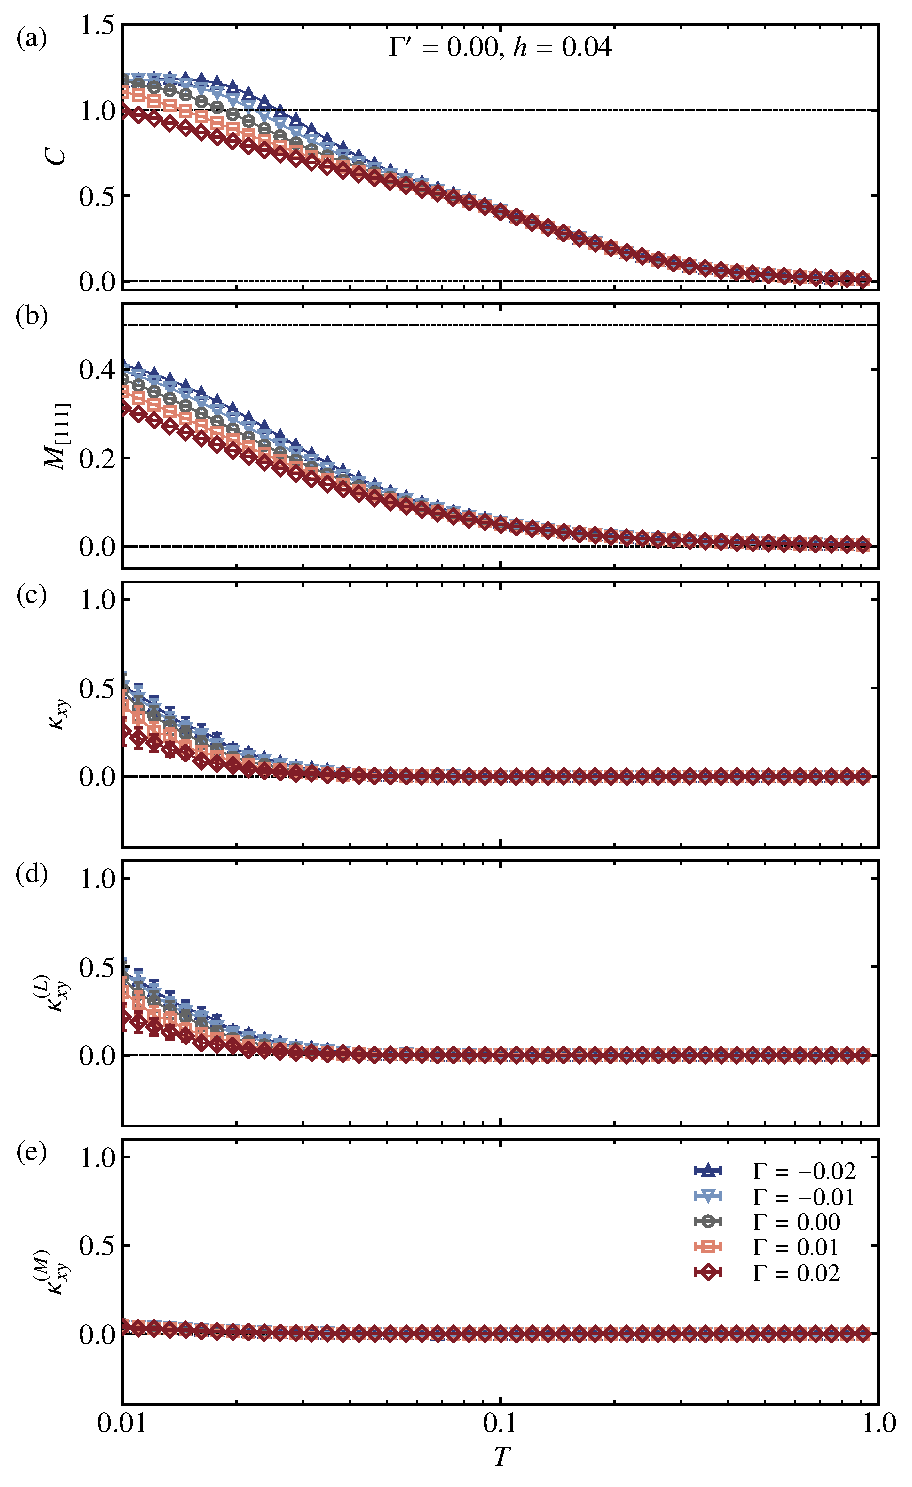
\includegraphics[width=0.9\linewidth]{Figs/fig_K-1.0_Gp0.00_h0.04.pdf}
\vspace{-0.5cm} 
\caption{Temperature dependence of (a) the specific heat, (b) the total magnetization, and
(c) the thermal Hall conductivity $\kappa_{xy}$ in the classical Kitaev-$\Gamma$ model under the magnetic field with $h=0.04$.
(d),(e) Temperature dependence of the two components, $(L)$ and $(M)$, of the thermal Hall conductivity.}
\label{fig_classical_gdep004}
\end{center}
\end{figure}

% \begin{figure}[tbh] 
% \begin{center} 
% 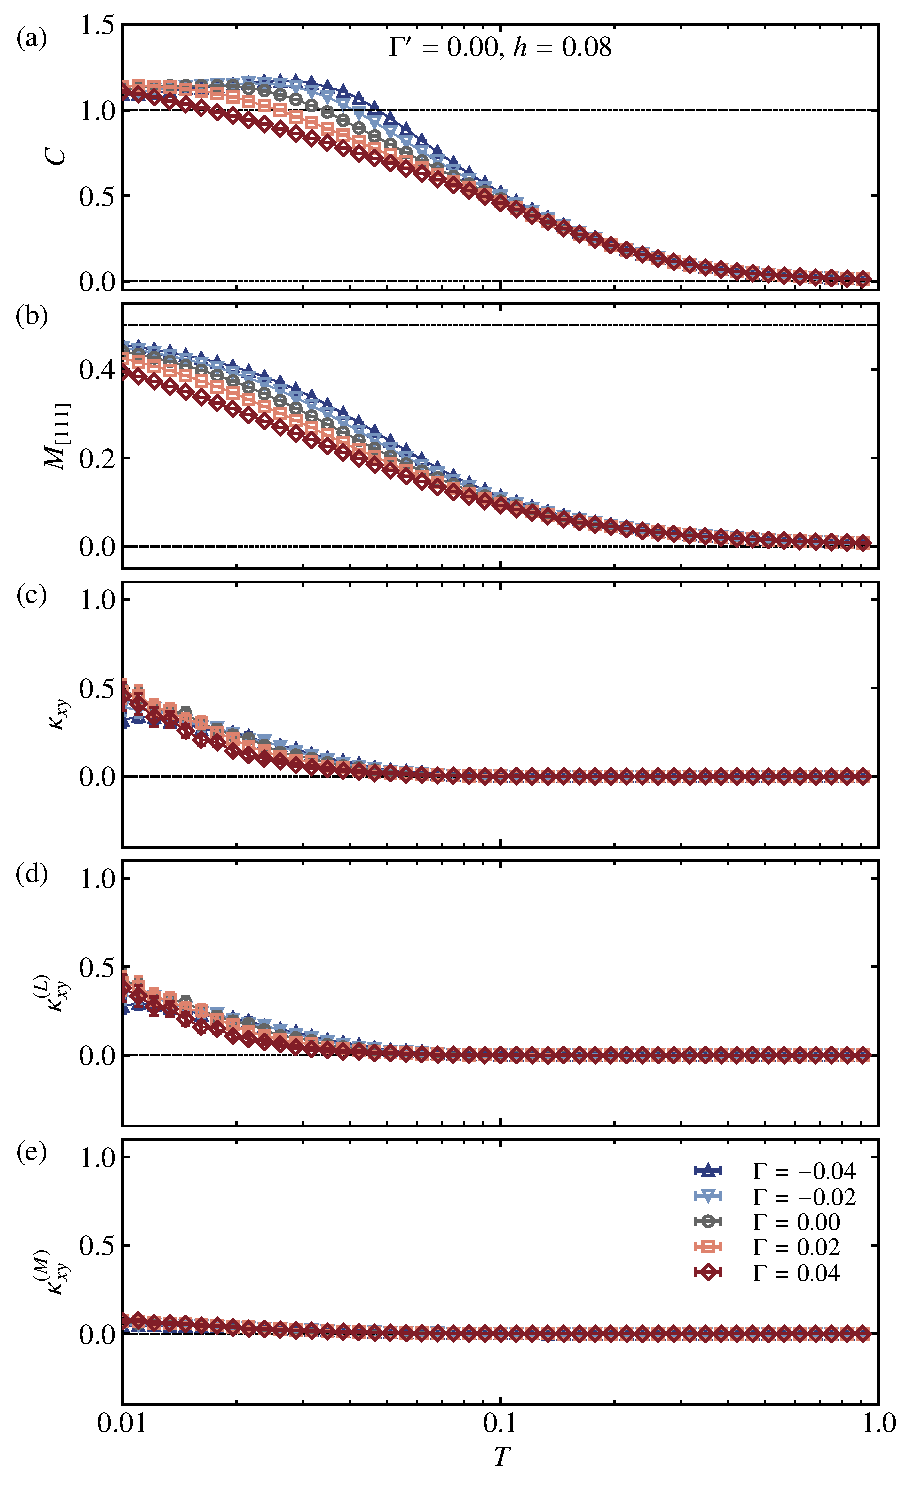
\includegraphics[width=0.9\linewidth]{fig_K-1.0_Gp0.00_h0.08.pdf}
% \vspace{-0.5cm} 
% \caption{Temperature dependence of (a) the specific heat, (b) the total magnetization, and
% (c) the thermal Hall conductivity $\kappa_{xy}$ in the classical Kitaev-$\Gamma$ model under the magnetic field with $h=0.08$.
% (d),(e) Temperature dependence of the two components, $(L)$ and $(M)$, of the thermal Hall conductivity.}
% \label{fig_classical_gdep008}
% \end{center}
% \end{figure}
  



% \begin{figure}[tbh] 
% \begin{center} 
% 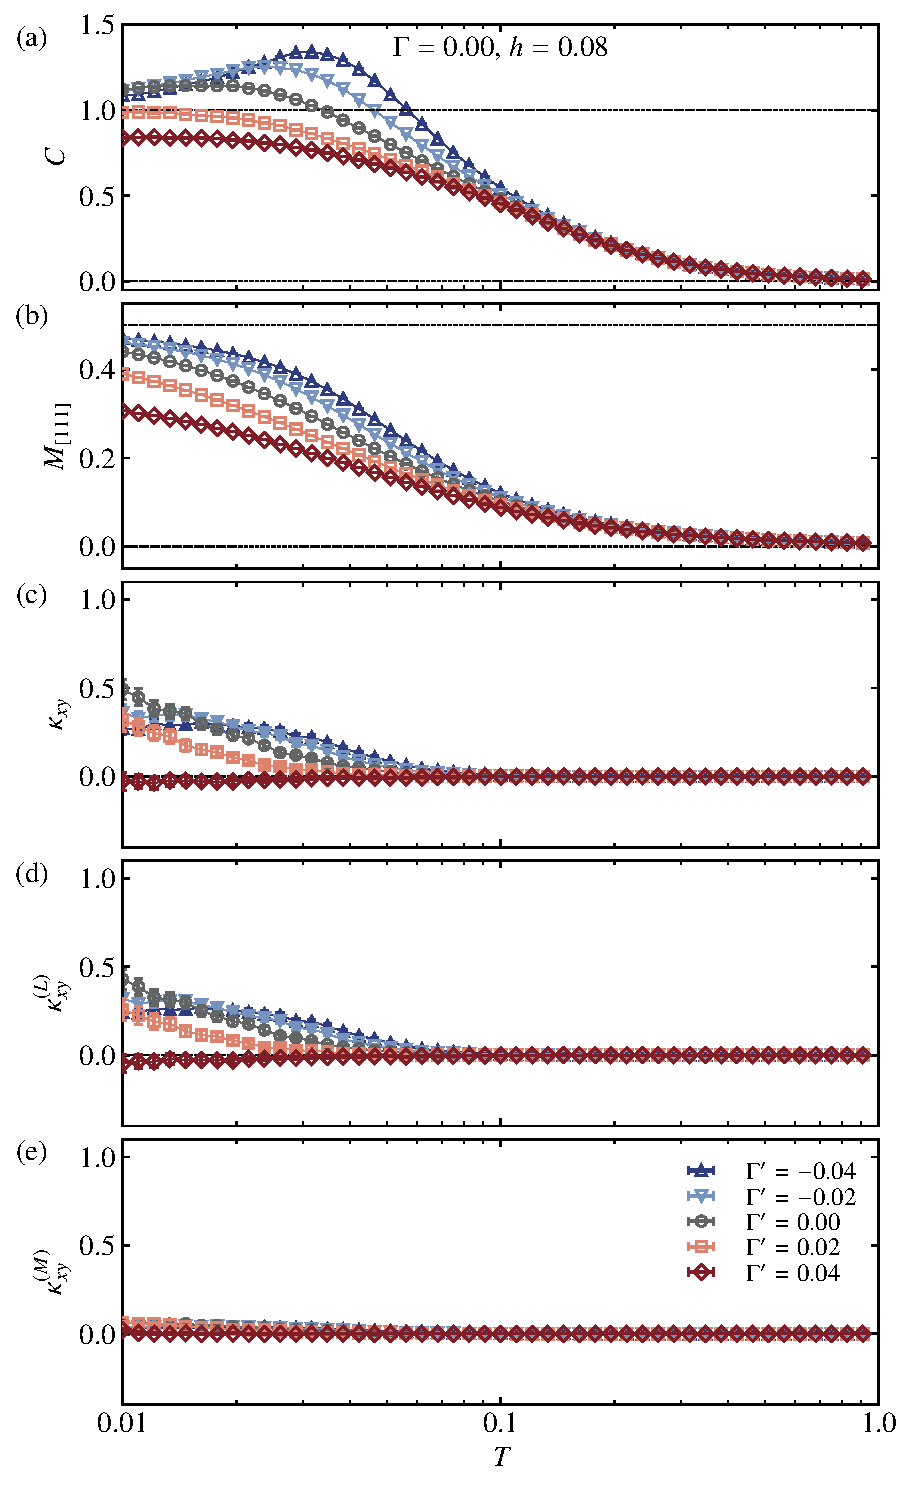
\includegraphics[width=0.9\linewidth]{fig_K-1.0_G0.00_h0.08.pdf}
% \vspace{-0.5cm} 
% \caption{Temperature dependence of (a) the specific heat, (b) the total magnetization, and
% (c) the thermal Hall conductivity $\kappa_{xy}$ in the classical Kitaev-$\Gamma'$ model under the magnetic field with $h=0.08$.
% (d),(e) Temperature dependence of the two components, $(L)$ and $(M)$, of the thermal Hall conductivity.}
% \label{fig_classical_gpdep008}
% \end{center}
% \end{figure}

%\clearpage
\subsection{Summary of temperature field dependence}
In this section, we summarize the temperature and %the magnetization 
magnetic field 
dependence of $\kappa_{xy}$ in both quantum and classical systems.
In Figs.~\ref{fig:color_map_all},
we %summarize 
show the two-dimensional color plots of $\kappa_{xy}/T$ %varying the 
as functions of temperature and %the 
magnetic field for various values of $\Gamma$ and $\Gamma'$, respectively. 
%As we saw in the discussion based on the representative magnetic fields, depending on the sign and the strength of the symmetric off-diagonal interactions, $\kappa_{xy}/T$ shows a variety of features. 
First, we %can see 
observe that %there are peak structures 
peaks in $\kappa_{xy}/T$ appear in the $h$-$T$ plane.
%for wide parameter regions and 
We note that the peaks %heights %can 
overshoot the half-quantized value. 
By introducing a weak $\Gamma^{\prime}$ interaction to the pure Kitaev model, 
%the 
a strong enhancements of $\kappa_{xy}/T$ %are 
is observed for negative $\Gamma'$, while positive $\Gamma'$ suppresses $\kappa_{xy}/T$. 
The negative $\kappa_{xy}/T$ observed for smaller $h$ and lower temperature %are 
is probably due to the small $D$ effects.
%When we introduce 
In the case of $\Gamma$,
we %can see 
observe that negative $\Gamma$ suppresses $\kappa_{xy}/T$, 
%while 
whereas positive $\Gamma$ %can largely 
significantly enhances it %for 
at high magnetic fields. 
In addition, positive $\Gamma$ %clearly introduces 
makes $\kappa_{xy}/T$ negative at small magnetic fields. 
By comparing $\Gamma = 0.01$ and $0.02$, we %realize 
observe that the region of negative $\kappa_{xy}/T$ moves to higher magnetic fields. This trend might be related to a possible quantum phase transition, as discussed above. 
%our numerical calculation. 
%\textcolor{red}{(Probably, we need to discuss the results both of quantum and classical models. However, so far, I wrote only quantum part.)}

In Fig.~\ref{fig:cmap_classical}, we show the color plot of $\kappa_{xy}$ in the $h$-$T$ plane of the classical model. 
We can see that $\Gamma$ term do not affects the overall behavior of $\kappa_{xy}$, 
while negative (positive) $\Gamma^{\prime}$ enhance (diminish) $\kappa_{xy}$.
The insensitivity to the Γ term is in contrast to the results for quantum systems.
Thus, the effects of $\Gamma$ term are governed by the
quantum effects while those of $\Gamma^{\prime}$ can be captured by the
classical model. 

%\blue{[古典の結果は0.01がなかったのでとりあえず0.04までにしています。追加計算中であとで改訂します。
%古典系の場合は量子化をしないので、$\kappa_{xy}$を温度で割らずにプロットしているのに加えて、$\Gamma$正のときに負にならないので、あまり比較にならないかもしれません。]}\red{ (新しい図%をもらって差し替えました。)}

\begin{figure*}[htb]
  \begin{center}
    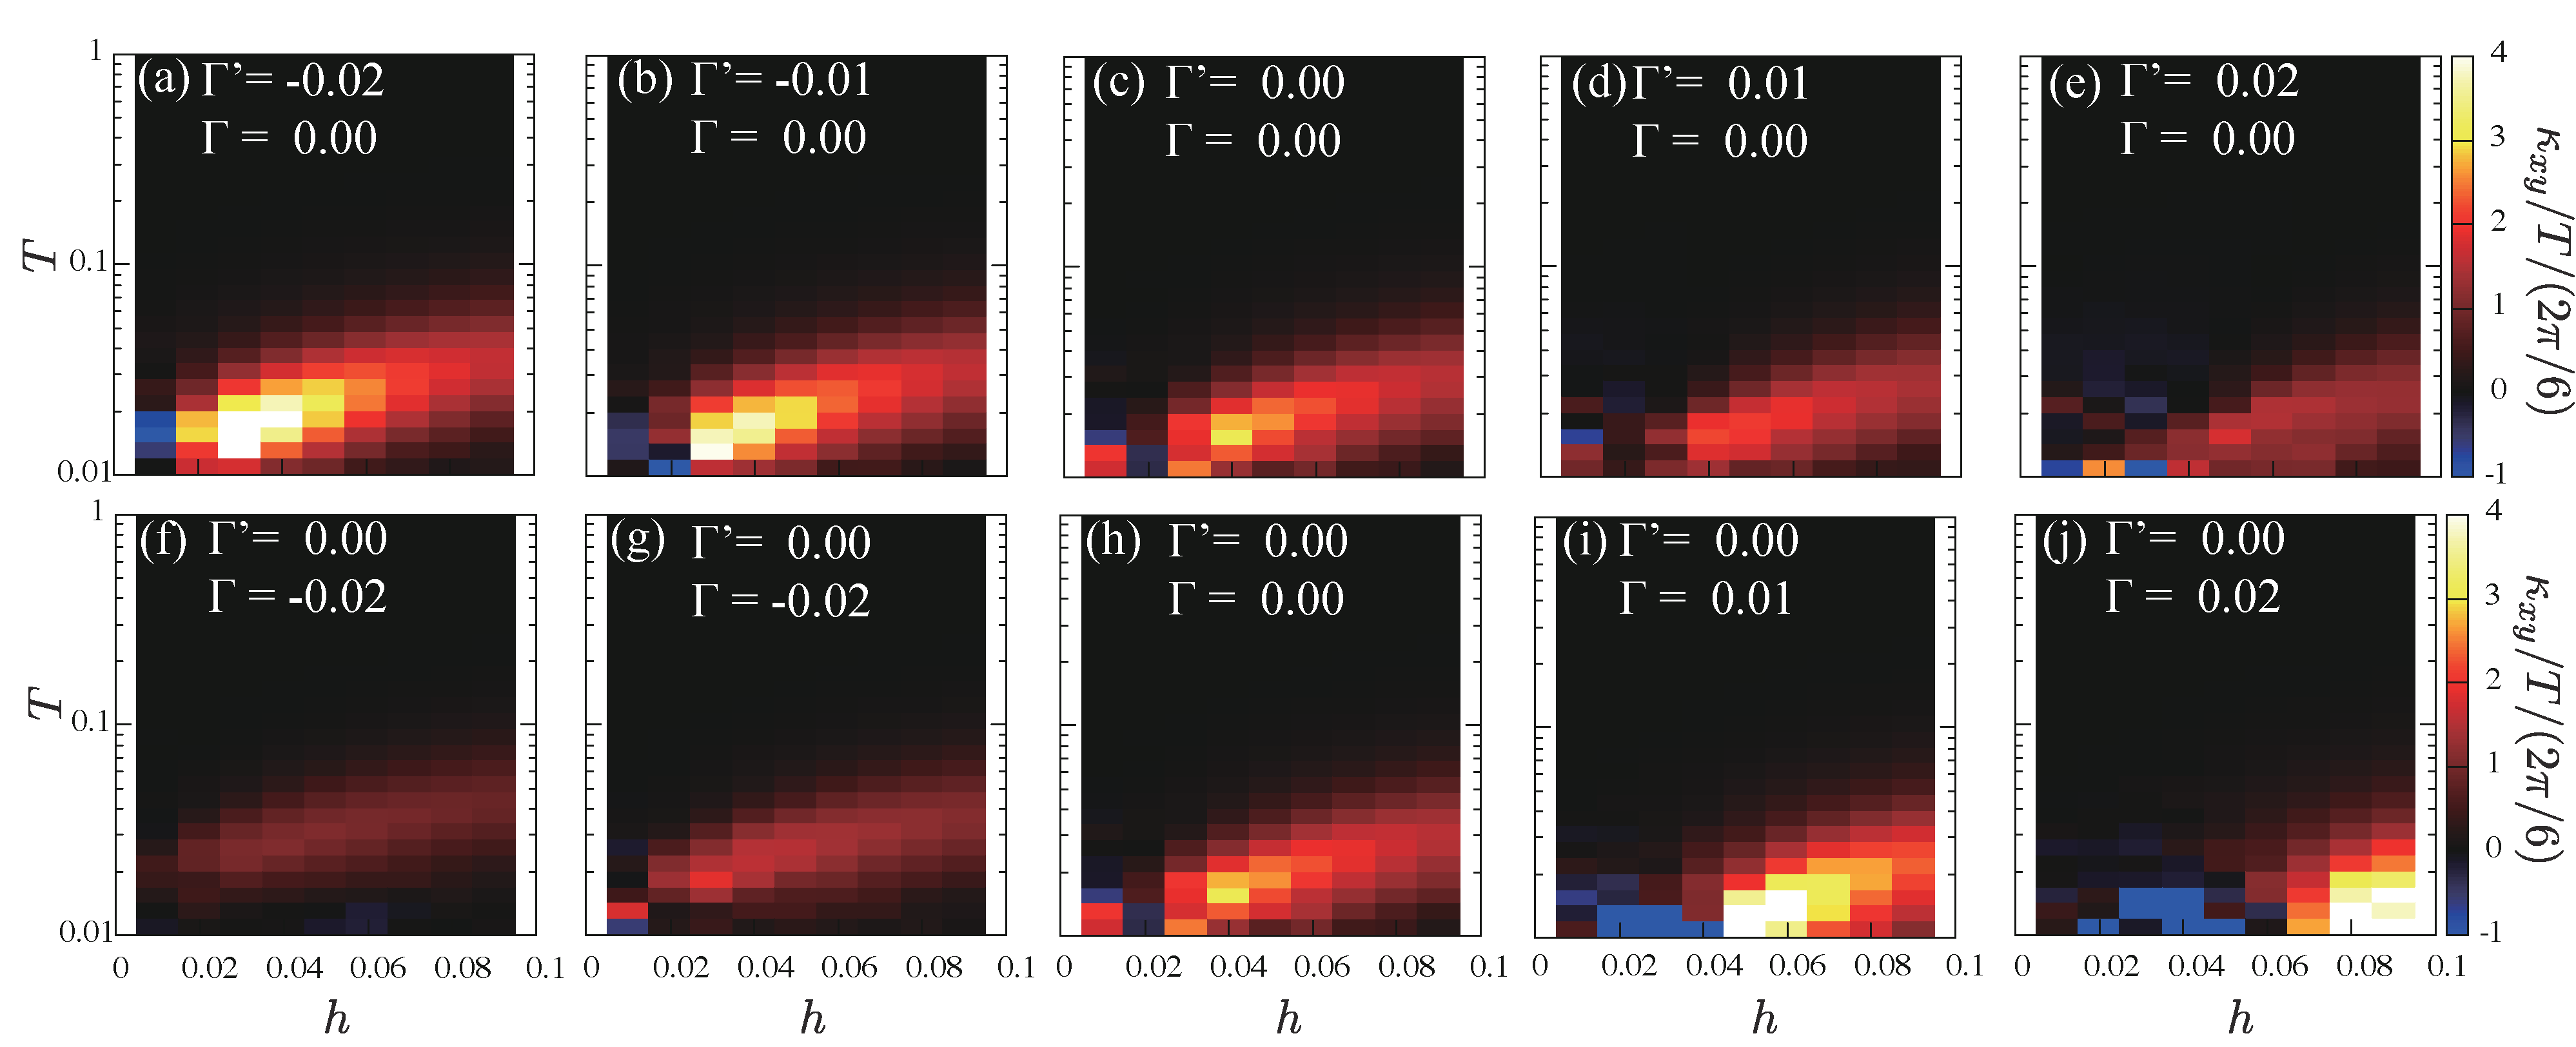
\includegraphics[width=\linewidth]{Figs/color_map_all.pdf}
  \end{center}
  \caption{(a)-(e)~Color maps of $\kappa_{xy}/T$ for ferromagnetic Kitaev model with $\Gamma = 0, \pm 0.01, \pm 0.02$ with various magnetic fields and temperatures.
  (f)-(j)~Color maps of $\kappa_{xy}/T$ for ferromagnetic Kitaev model with $\Gamma' = 0, \pm 0.01, \pm 0.02$ with various magnetic fields and temperatures.}
  \label{fig:color_map_all}
\end{figure*}

%\begin{figure*}
%  \begin{center}
%    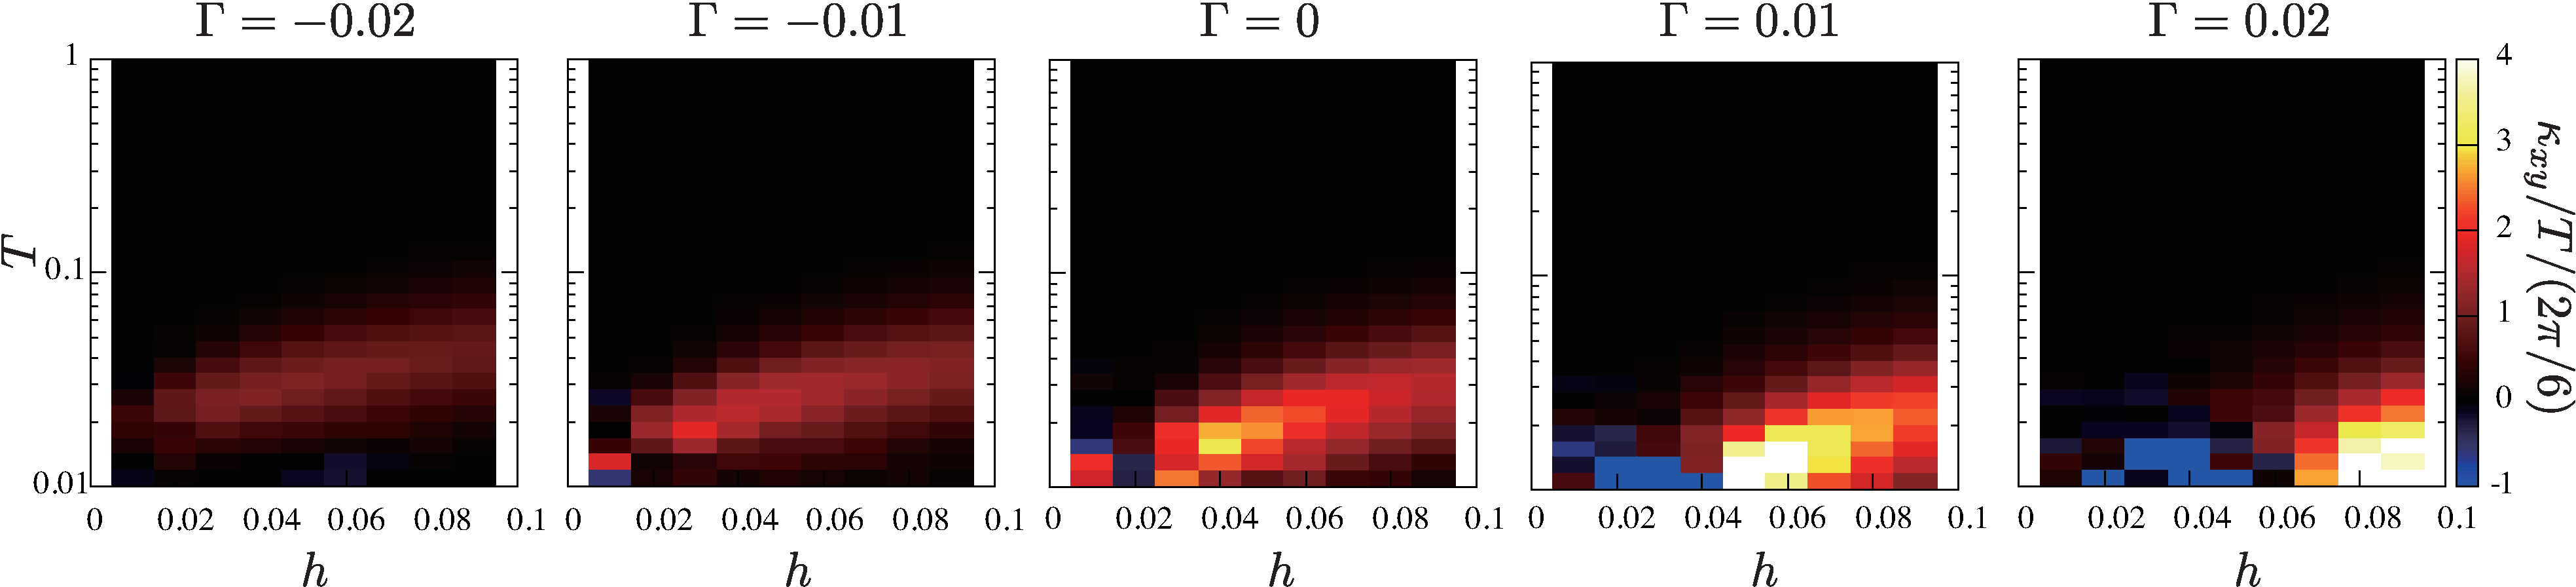
\includegraphics[width=\linewidth]{Figs/color_map_G.pdf}
%  \end{center}
%  \caption{Color maps of $\kappa_{xy}/T$ for ferromagnetic Kitaev model with $\Gamma = 0, \pm 0.01, \pm 0.02$ with various magnetic fields and temperatures.}
%  \label{fig:color_map_G}
%\end{figure*}

\begin{figure*}
  \begin{center}
    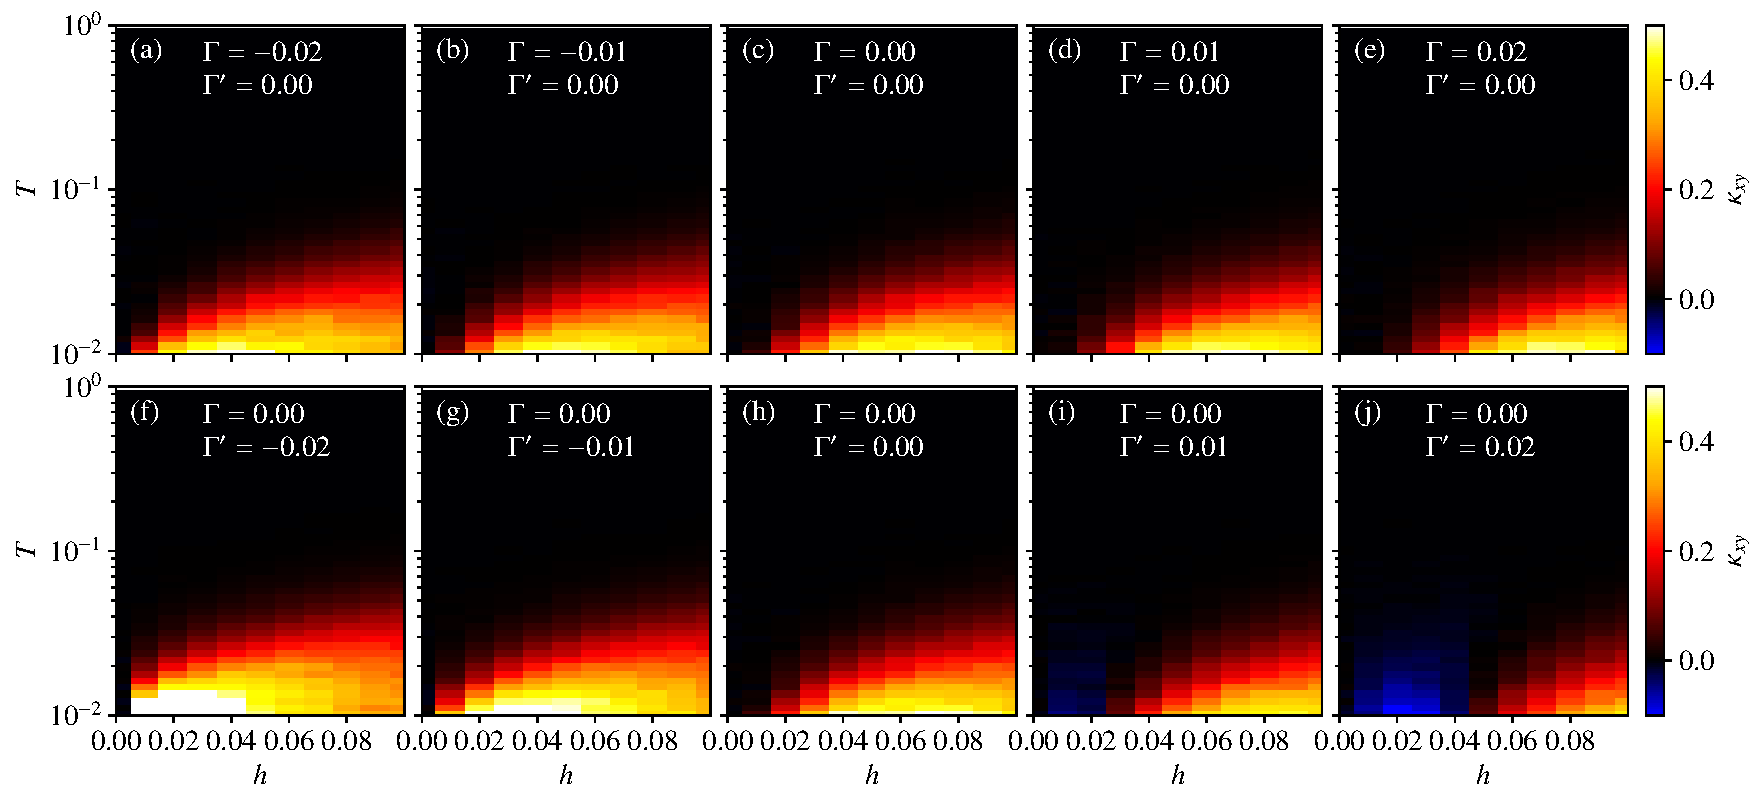
\includegraphics[width=\linewidth]{Figs/fig_cmap_classical.pdf}
  \end{center}
  \caption{
   Corresponding plots to Fig.~\ref{fig:color_map_all} for the classical model.
   %\blue{Color maps of $\kappa_{xy}$ for the ferromagnetic Kitaev model with several values of $\Gamma$ and $\Gamma'$ on the plane of the magnetic field and temperature.}
   }
  \label{fig:cmap_classical}
\end{figure*}

%\clearpage
\section{Summary and Discussion}
\label{sec:Summary}
%\red{セクションのタイトルにDiscussionを入れてみました。}
In this study, we %showed 
have conducted a systematic analysis of thermal Hall conductivity 
in the extended Kitaev model at finite temperatures using the tensor-network 
representation of the density matrix. 
This method enables %us to perform 
a highly-accurate analysis of the
thermal Hall conductivity beyond %the 
conventional perturbation theory. 
%The significant 
A key finding of this study is that the thermal Hall conductivity %largely 
significantly exceeds the half-quantized value. 
This result indicates that the large thermal Hall conductivity observed in $\alpha$-RuCl$_3$ experiments 
can be %explained by the physics 
understood within the framework of the Kitaev model. 
We have demonstrated that the field-angle dependence of the thermal Hall conductivity remains consistent with the sign of the Chern number 
of Majorana fermions even in the high-magnetic-field regime.
%In the case of 
For the thermal Hall conductivity induced by the topological magnon, %the 
its sign is opposite to %the present results 
that observed in the present study~\cite{McClarty_PRB2018}. 
In %addtion 
addition to the sign, its magnitude is smaller than the half-quantized value, indicating that the %toplogical 
topological magnon alone may %might 
not be able to explain the overshooting of the thermal Hall conductivity.

% \red{これって、Majoranaでなくても、ハミルトニアンの対称性から議論できるのではなかったでしたっけ?その場合、Majoranaとconsistentなことを強調するのはmisleadingな気がします。}
% \orange{基底状態がKitaev QSLではなくなっている高磁場側でも符号が整合
% するのはnon trivialだと思ったのですが、どうでしょう?
% 古典系でも符号はあってしまっているのでそこは気になるのですが。
% むしろ、Majorana的な振る舞いが思っていたより頑強ということを強調したほうが
% よいでしょうか?
% }
% \blue{少なくともMagnonの場合は、Ref.~\cite{McClarty_PRB2018}によれば、[111]磁場で高磁場領域で、Kが0.3くらいで熱ホール係数の絶対値がピークを取り、符号は負ですので、それとはコンシステントではないと思います。
% この議論もここに付け加えても良いと思います。
% あとは、$\kappa^{xy}/T$のピークの値は-0.3くらいなため、$\pi/6$よりは小さいので、overshootingは説明できないように思います。それも次の段落に関係するので、文章として埋め込んでも良いかと思います。
% }
% \red{ありがとうございます。符号とovershootの議論、確かにおっしゃる通りだと思います。Zoomで議論できれば。}

Note that the overshoot of the thermal Hall conductivity beyond the half-quantized value has not been observed in the 
%previsou 
previous numerical study \cite{KumarT2023}. 
As we already mentioned, we have employed a proper position dependent representation for the poralization and have obtained the energy current as a vector, %while 
whereas the authors of %in 
\cite{KumarT2023} used a simplified treatment neglecting %a 
the directional dependence of energy currents. 
This treatment probably contributes to the significant difference in the calculated thermal Hall conductivities.


We %also show 
have also demonstrated that the thermal Hall conductivity is significantly affected by 
the $\Gamma$ and $\Gamma^{\prime}$ terms even when their %amplitudes 
magnitudes are two orders %of magnitude 
smaller than the Kitaev interaction. 
In particular, %in the case of the 
for negative $\Gamma^{\prime}$
and the positive $\Gamma$, 
the thermal Hall conductivity is enhanced.
However, %the origins of the 
the mechanisms behind this enhancement are quite different.
For negative $\Gamma^{\prime}$, 
we find that the enhancement is primarily driven by the three-body term $\kappa_{xy}^{(L)}$, %is the main contributor to the enhancement, 
which is consistent with the scenario %that 
where the negative $\Gamma^{\prime}$ term increases the Majorana gap~\cite{Takikawa_PRB2020}.
In contrast, %to this, 
for %the 
positive $\Gamma$, %case, 
the enhancement is governed by the two-body part $\kappa_{xy}^{(M)}$.
This mechanism %is not simply understood from the 
cannot be straightforwardly explained by
perturbation theory
and may be related to the possible phase transitions induced by the $\Gamma$ term.
By comparing %with 
the results in the quantum and classical systems, 
we find that the main effect of the $\Gamma^{\prime}$ term %can be captured 
is well captured by classical systems, 
whereas the effect of the $\Gamma$ term is not.
In other words, the behavior of the three-body part $\kappa_{xy}^{(L)}$ 
can be reproduced by the classical model, whereas $\kappa_{xy}^{(M)}$ cannot.
This result suggests that the $\Gamma$ term %has a larger 
exhibits stronger quantum effects.

%{\bf\orange{[実験との関連やtopological magnonとの関連の議論を追加する?]}}

Another important issue is the comparison %with 
between our results and the thermal Hall conductivity induced by topological magnons \cite{McClarty_PRB2018, Joshi_PRB2018, ChernZK2021}. 
Although we observed a finite thermal Hall conductivity even at 
higher temperatures, its sign is different from the calculations assuming topological magnons. The origin of this discrepancy is not fully clear at %the moment. 
moment. One possible origin might be the validity of the magnon picture at higher temperatures, where %we do not see small magnetization along the field direction.
the magnetization is small.
Another %possibility is 
possible explanation involves
the treatment of the edges in %the 
previous calculations %for the 
on topological magnons, %where they 
which assumed the bulk-edge correspondence and did not explicitly include the effects of the open edges, such as the reconstructions of magnetization around the edges \cite{KoyamaN2023,HabelMWK2024}.
%\blue{Magnon的な見方ではエッジモードのdamping (breakdown)に対応するかもしれませんので、もし可能であれば、PhysRevB.108.235162,PhysRevB.109.024441を引用いただければと思います。}
%\red{[とりあえず、番号だけ引用してみました。具体的な記述を追加するかは、相談させてください。]}
In contrast, in our calculation, we explicitly consider open boundaries and the thermal Hall conductivity is calculated %through 
based on the energy current at the edges. If the sign difference %in the sign really comes 
indeed originates from the edge treatment, our results might be relevant to the experimental observations because there are explicit edges in the experiments.

Our findings %highlight 
demonstrate the importance of developing methods that do not rely on specific quasiparticle assumptions. Most previous theoretical studies on the thermal Hall conductivity have focused on analyzing the contributions from the specific quasiparticles, such as the Majorana fermions and the topological magenons. In contrast, the method developed in this study enables the calculation of the thermal Hall conductivity in quantum spin systems without assuming specific quasiparticles. This approach provides a theoretical foundation for understanding experimental results, where the contributions from multiple quasiparticles may coexist. Given that thermal Hall conductivity measurements have been performed on a wide range of strongly correlated materials, our method offers a fundamental theoretical framework for their interpretation and serves as a useful tool for identifying exotic quasiparticles from experimental observations. This work paves the way for a more comprehensive understanding of the thermal Hall effect in strongly correlated materials.


\begin{acknowledgments}
We wish to thank Y. Kato, K. Fukui, and K. Ido for fruitful discussions.
%TM was supported by Building of Consortia for the Development of Human Resources in Science and Technology, MEXT, Japan.
This work was supported by  Grant-in-Aid for Scientific Research
Nos.~19H05825, 19K03742, 20H00122, 	22H01179, 23K22450, and  23H03818 from the Ministry of Education, Culture, Sports, Science and Technology, Japan.
It is also supported by JST CREST Grant No.~JPMJCR18T2, JST PRESTO Grant No.~JPMJPR19L5, and JST COI-NEXT Program Grant Number JPMJPF2221. This work was also supported by the National Natural Science Foundation of China (Grant No.~12150610462). Numerical calculations were performed using the facilities of the Supercomputer Center, The Institute for Solid State Physics, The University of Tokyo.
\end{acknowledgments}

%\clearpage
\appendix
\section{Benchmark on tensor network method}
\label{app:XTRG_Bench}
In this Appendix, we present several benchmark %calculations 
results for the XTRG method. 
First, we show %bond-dimension 
dependence of the several representative 
physical quantities on bond dimension $D$ %of 
for the pure Kitaev model on the $(L, L') = (6, 6)$ cylinder 
%for bond-dimensions $D=300$, $400$, and $D=500$ 
in Fig.~\ref{fig:CMk_XC6}. 
%We showed the data for $D=500$. 
We find that %$D$ dependence 
the dependence on $D$ becomes larger %for $T \lesssim 0.05$
for the specific heat and the thermal Hall conductivity %in
at $h=0.04$ when $T \lesssim 0.05$.
However, %in 
for $D=500$, 
clear peak structures appear in the specific heat and the thermal Hall conductivity %in $D=500$ 
and their values %are not so deviated 
deviate from those %of 
at $D=400$. 
Thus, we conclude %consider 
that %the 
$D=500$ is sufficiently large to %discuss 
analyze the thermal Hall conductivity %and related physics 
for $(L, L') = (6, 6)$, $T\geq 0.01$, and $h\geq 0.04$.

Next, for %another 
a different system size $(L, L') = (8, 4)$, 
we examine the bond-dimension dependence of the physical quantities.
As shown in Fig.~\ref{fig:CMk_XC4}, 
for $D$ up to $400$, we obtained almost converged data even for the specific heat and the thermal Hall conductivity at $h=0.04$. 
Although the accuracy of the matrix product representation depends on the circumference, i.e., the system size, we can obtain %the almost 
nearly converged results
for $D=400$. These results demonstrate that the XTRG method with a sufficiently large bond dimension
$D$ is a powerful tool for investigating the finite-temperature properties of quantum spin systems.

\begin{figure}[htb]
  \begin{center}
    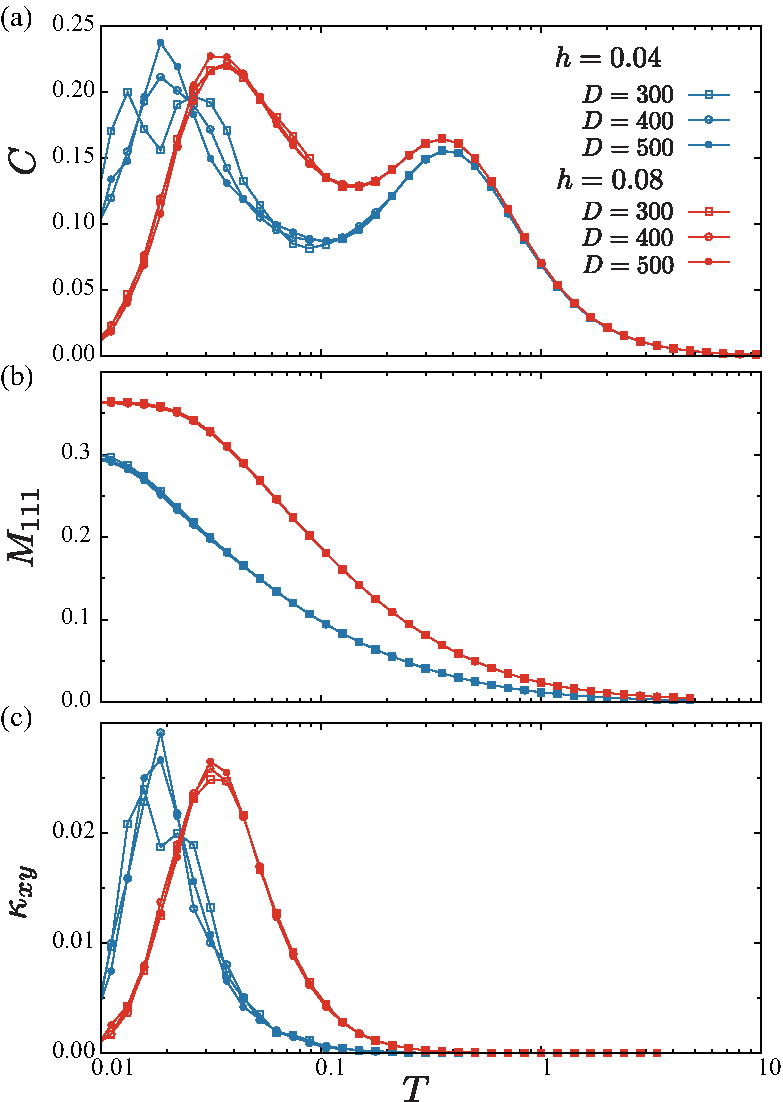
\includegraphics[width=0.9\linewidth]{Figs/plot_CMk.pdf}
  \end{center}
  \caption{Temperature dependence of (a) the specific heat (b) the magnetic moment, and (c) the thermal Hall conductivity of the ferromagnetic Kitaev model for the external magnetic field $h=0.04$ and $h=0.08$ parallel to $[111]$ direction with different bond-dimensions $D=300, 400, 500$. The lattice is $(L, L') = (6, 6)$}
  \label{fig:CMk_XC6}
\end{figure}

\begin{figure}
  \begin{center}
    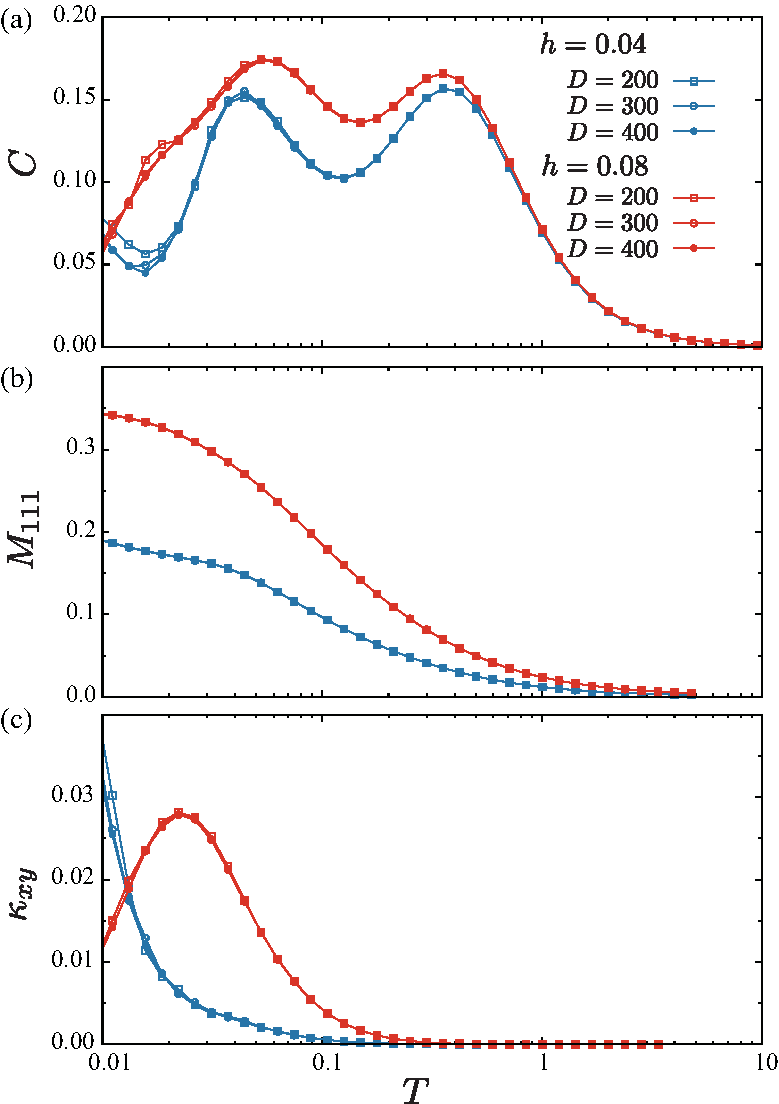
\includegraphics[width=0.9\linewidth]{Figs/plot_CMk_XC4.pdf}
  \end{center}
  \caption{Corresponding plot to Fig.~\ref{fig:CMk_XC6} for $(L, L') = (8, 4)$.} 
  %Temperature dependence of (a) the specific heat (b) the magnetic moment, and (c) the thermal Hall conductivity of the ferromagnetic Kitaev model for the external magnetic field $h=0.04$ and $h=0.08$ parallel to $[111]$ direction with different bond-dimensions $D=200, 300, 400$. The lattice is \red{$(L, L') = (8, 4)$}.}
  \label{fig:CMk_XC4}
\end{figure}




%\clearpage
\section{Benchmark on thermal pure quantum state}
\label{app:cTPQ}
%\orange{{\bf この節はそもそもいらない気がしますが...}$\to$とりあえず、情報はあっても良いと思ったので、残しています}
In this Appendix, we examine the accuracy of the cTPQ method %in this section
by comparing %the results of the cTPQ method 
its results with those of
%the 
full diagonalization for a small $(L, L') = (2, 4)$ cluster (the total system size is $N_{\rm s}=16$).
In the full exact diagonalization (ED) method, we diagonalize the Hamiltonian, whose dimension is
$2^{16}=65536$ using ScaLAPACK~\cite{scalapack}. 
Using the obtained eigenvalues and eigenvectors,
we calculate the temperature dependence of %the 
physical quantities.

At $h=0.04$, the specific heat $C$ exhibits a three-peak structure in this system size.
This structure may be an artifact of the small system size 
since it %vanishes 
disappears %for 
in larger system sizes.
Even at $h=0.08$, %the 
a hump in the specific heat %still exists 
remains around $T=0.02$.
As shown in Fig.~\ref{comp_ED}(a),
the cTPQ method reproduces the temperature dependence 
of the specific heat for $h=0.04$ and $h=0.08$, including
its three-peak structure.
Figure~\ref{comp_ED}(b) shows the temperature dependence of the magnetization.
The cTPQ method also reproduces the results of full exact diagonalization. 

\begin{figure}[t] 
\begin{center} 
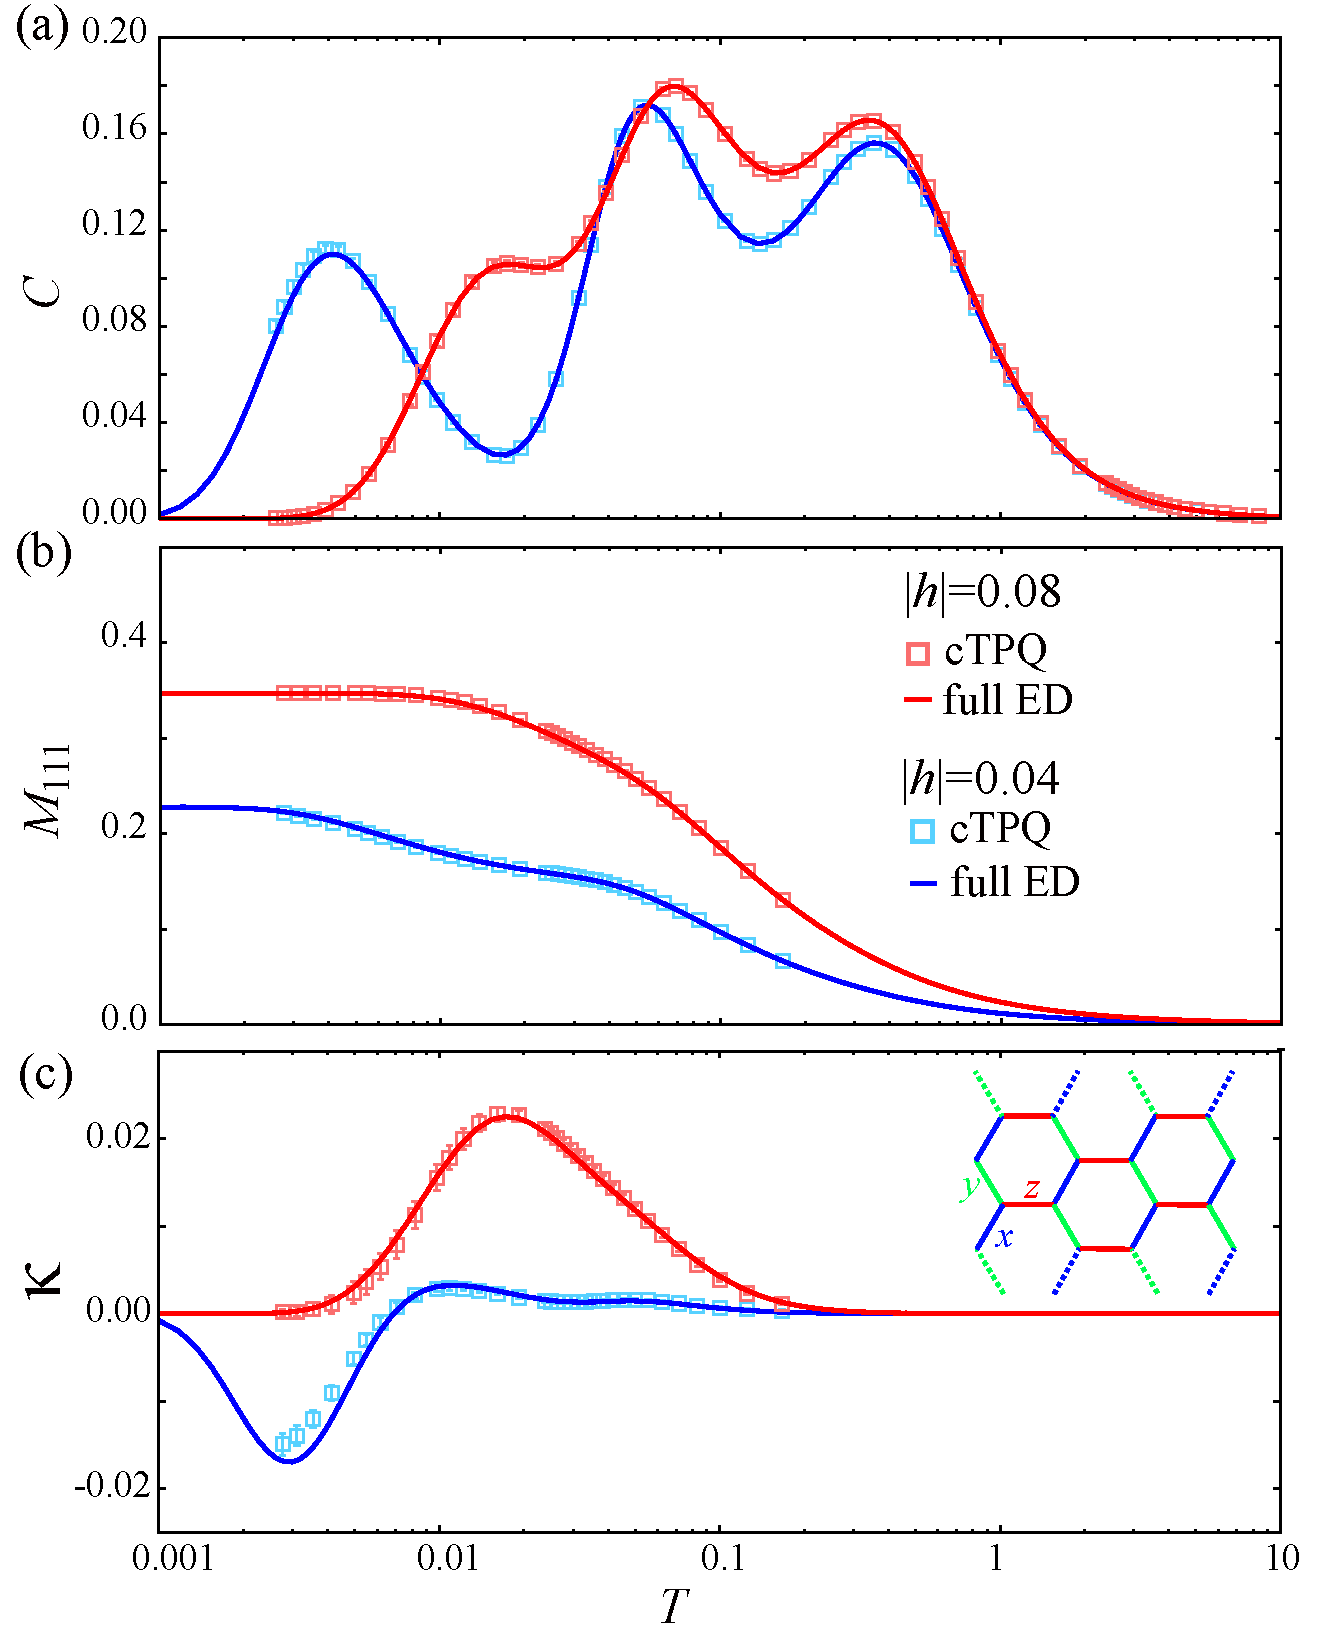
\includegraphics[width=0.9\linewidth]{Figs/compED_4_o.pdf}
\vspace{-0.5cm} 
\caption{Temperature dependence of (a) the specific heat, (b) the total magnetization, and
(c) the thermal Hall conductivity $\kappa$.
In the bootstrap sampling, we take $1000$ independent initial states and choose $1000$ samples $500$ times with replacement to evaluate
the average values and the error vars.
%We take $N_{\rm tot}=P=1000,M=500$ in the bootstrap sampling.
}
\label{comp_ED}
\end{center}
\end{figure}

We show the temperature dependence of the thermal 
Hall conductivity $\kappa$ in Fig.~\ref{comp_ED}(c).
The thermal Hall conductivity $\kappa$ at $|h|=0.04$
becomes negative for $T\leq 0.01$. This negative $\kappa$ may also %be 
%caused by the 
result form finite-size effects, possibly due to the short length of the edges.
In fact, $\kappa$ becomes positive for larger system sizes, as we %show 
demonstrated above.
The cTPQ method %well reproduces this peculiar temperature dependence. 
accurately captures this unusual temperature dependence.
At $h=0.08$, $\kappa$ shows 
a single peak, %and it is also well 
which is also accurately reproduced by the cTPQ method.
%These consistencies 
This agreement with %the results of the 
full diagonalization demonstrate
the %validity 
reliablity of the cTPQ method.

\section{Comparison between tensor network method and thermal pure quantum state}
\label{app:XTRGcTPQ}
In this Appendix, we examine the accuracy of the XTRG method
by comparing the results of the cTPQ method with those of the XTRG
for the $(L, L') = (6, 2)$ cluster ($N_{\rm s}=24$). 
Figure~\ref{comp_XTRG}(a) shows the temperature dependence of the specific heat. 
We find that both methods reproduce the two-peak structure in the specific heat, which is a 
characteristic feature %in 
of the Kitaev model. 
%Except for the 
Apart from a small discrepancy %around 
near the low-temperature peak 
at $h=0.04$, both methods %agree well with each other
show good agreement across three orders of magnitude in temperature.
%over the three magnitudes of the temperature scale.
This consistency demonstrates that the XTRG method, with a sufficiently large 
bond dimension, 
%gives 
provides accurate results.

In Fig.~\ref{comp_XTRG}(b),
we show the temperature dependence of the magnetization.
%In 
Across all the temperature regions, 
we find that both methods %agree well 
show good agreement within the error bars.
Since the magnetization is given by the first derivative of the
free energy, its fluctuations are expected to be small.
This may %be the reason 
explain why the error bars of the magnetization
are smaller than those of the specific heat and the thermal Hall conductivity.

We show the temperature dependence of $\kappa$
in Fig.~\ref{comp_XTRG}(c) and find that
$D=500$ already %gives 
provides sufficiently accurate
results of the thermal Hall conductivity $\kappa$ except for the small deviations %on 
in its peak values. 
%the peak values of $\kappa$. 
%This result 
These results indicate that  
the XTRG calculations %shown 
presented in this paper %correctly 
accurately capture the %essence 
essential features of the
thermal Hall conductivity in %the 
extended Kitaev models. 

\begin{figure}[tbh] 
\begin{center} 
%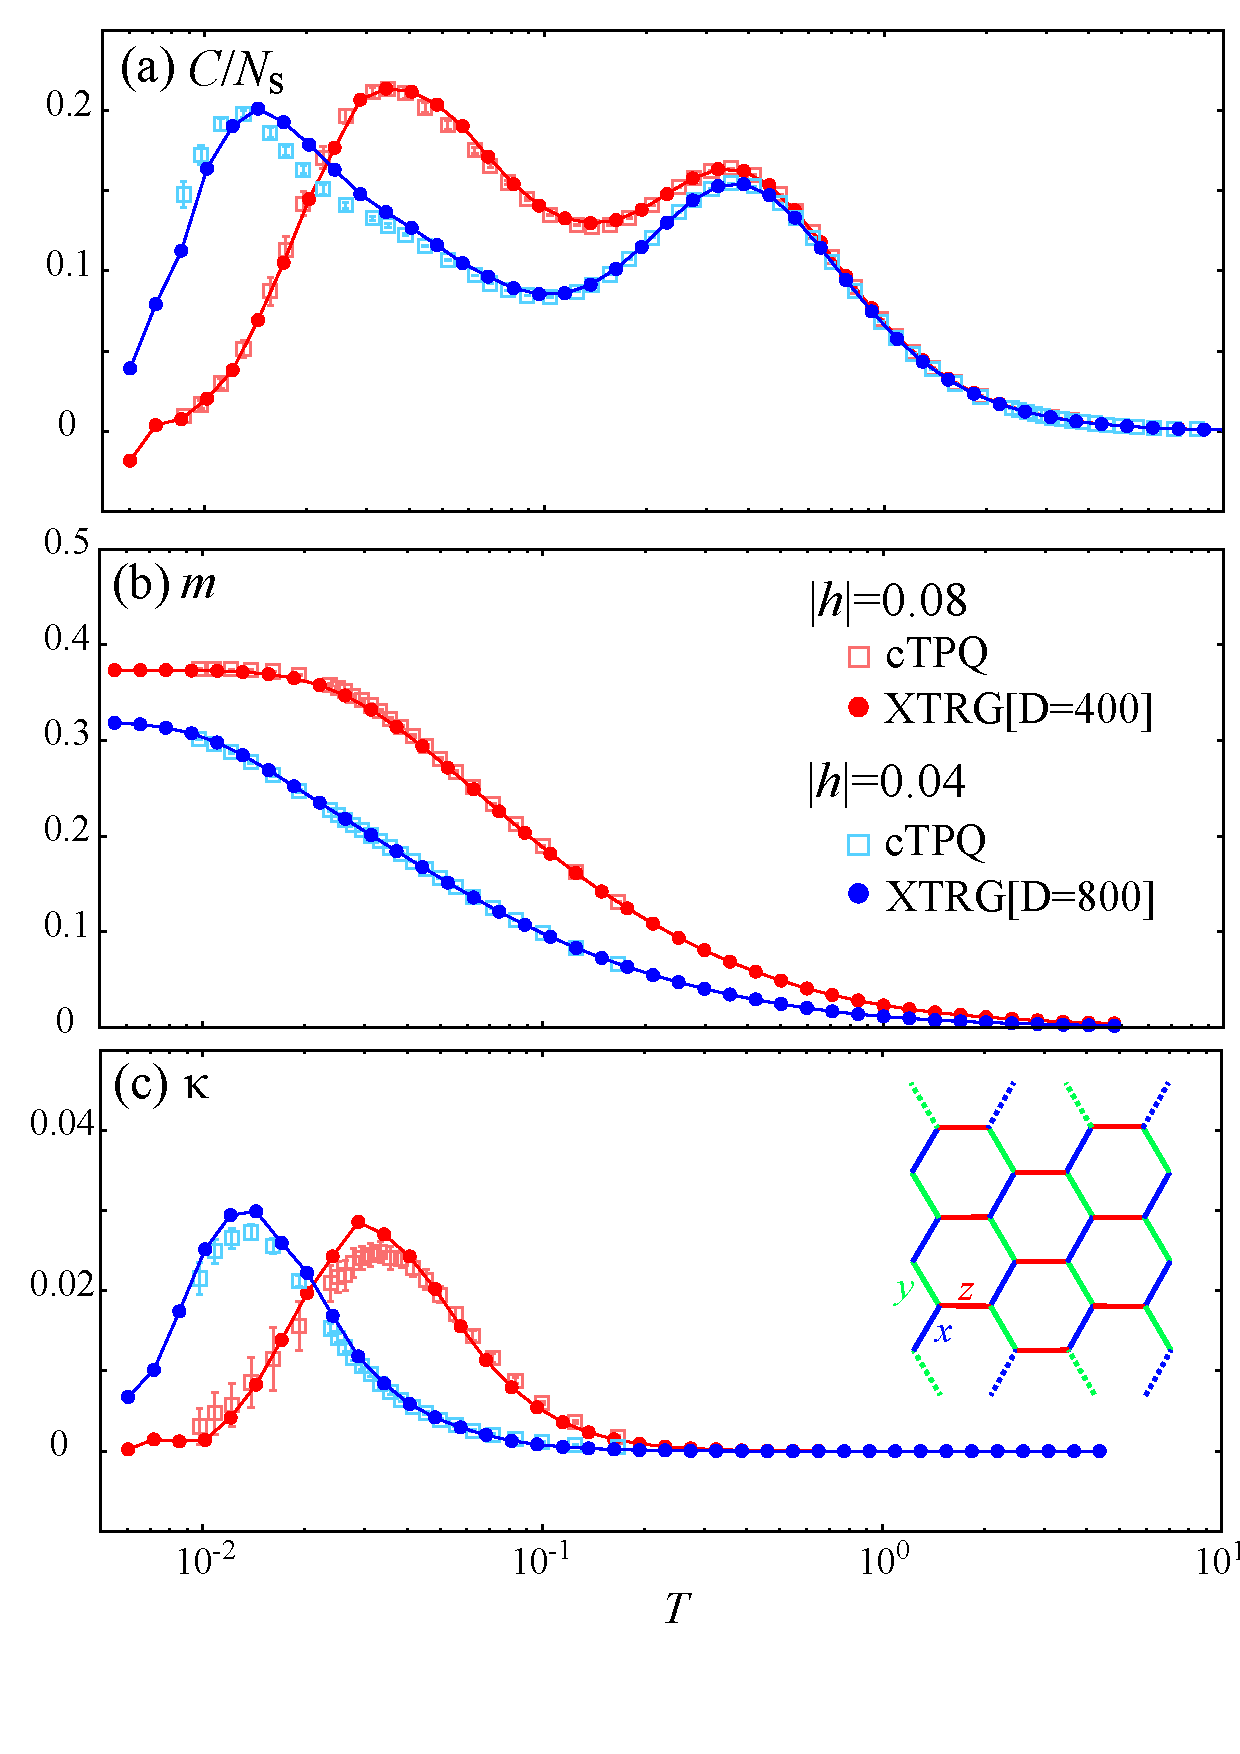
\includegraphics[width=0.9\linewidth]{comp_XTRG_o.pdf}
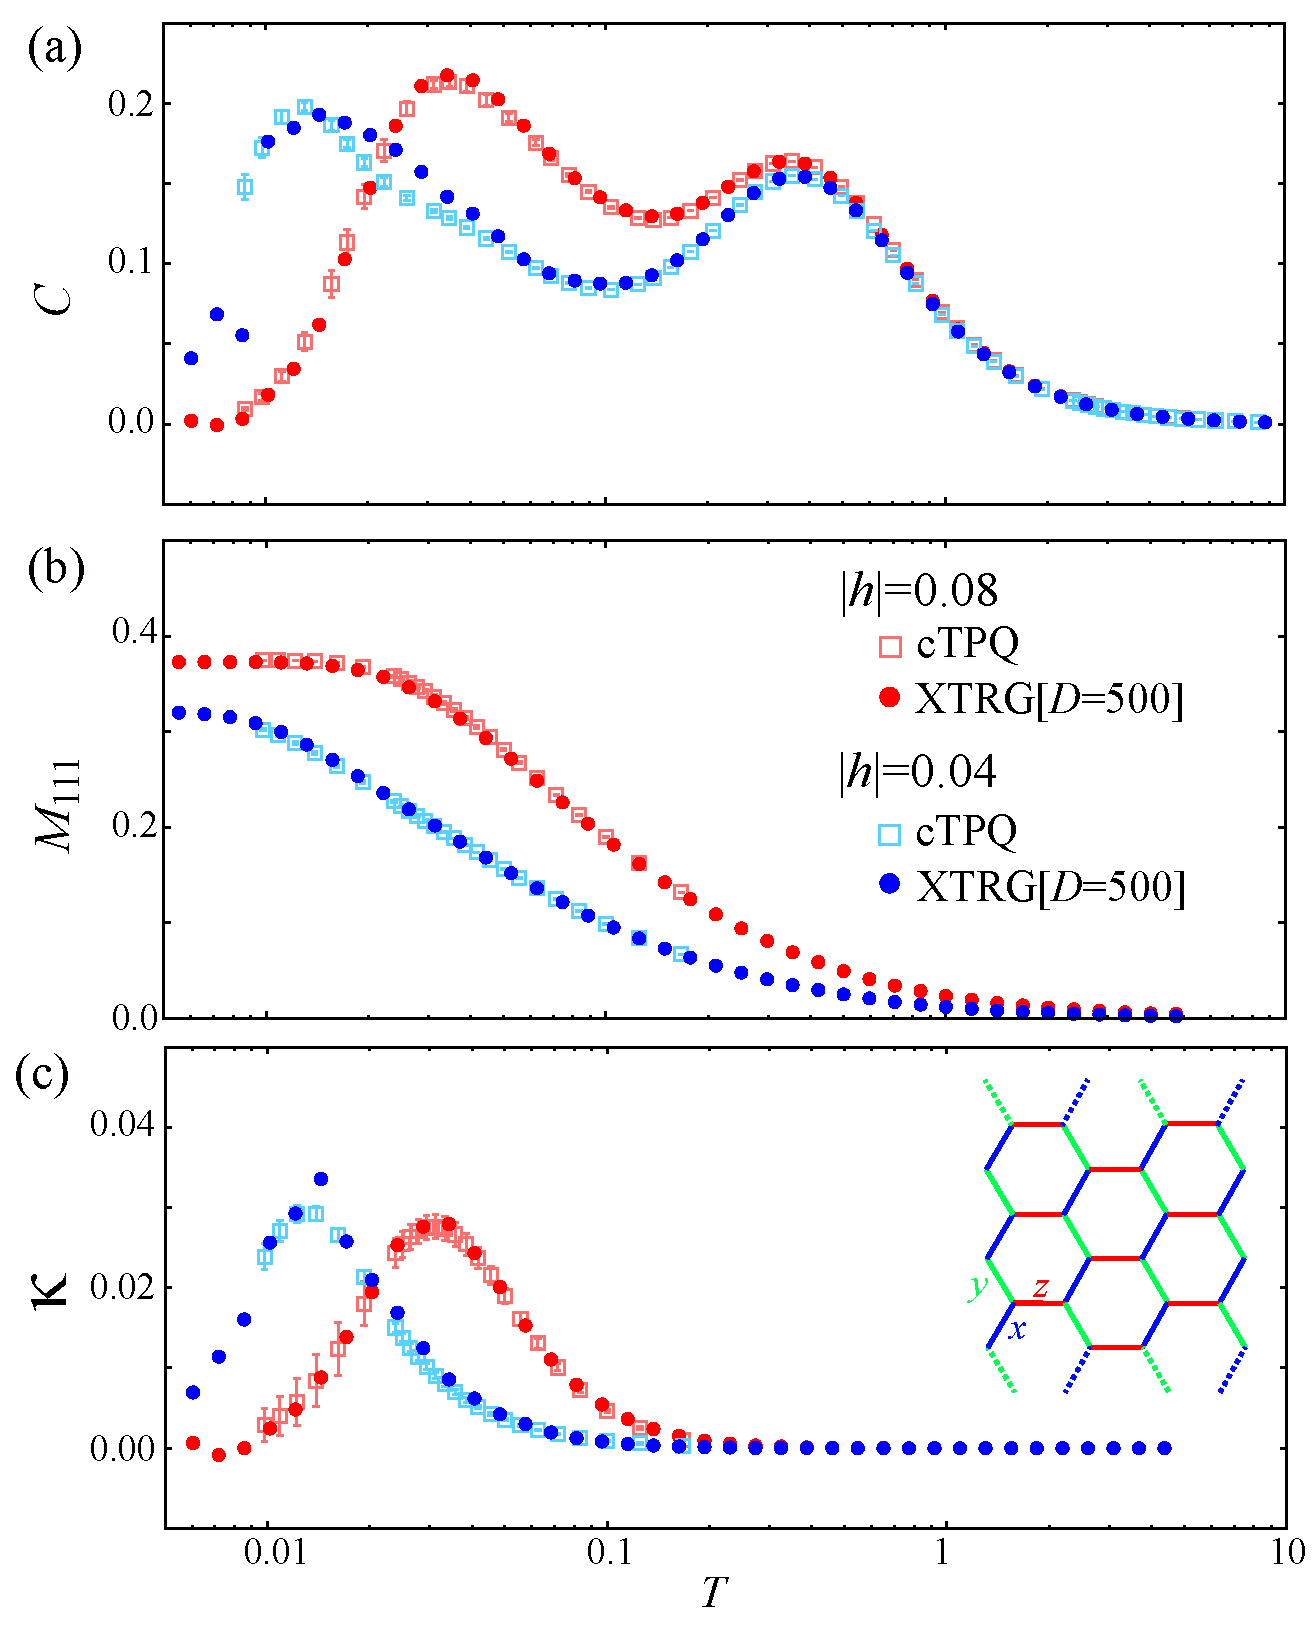
\includegraphics[width=0.9\linewidth]{Figs/compXTRG_3_o.pdf}
\vspace{-0.5cm} 
\caption{Temperature dependence of (a) the specific heat, (b) the total magnetization, and
(c) the thermal Hall conductivity $\kappa$. 
In the bootstrap sampling, we take $100$ independent initial states,
and choose $100$ samples $50$ times with replacement to evaluate
the average values and the error vars.
}
\label{comp_XTRG}
\end{center}
\end{figure}


% \clearpage
% \section{Field-angle dependence of physical quantities}
% \label{app:fieldangle}

% \clearpage

%{\bf \orange{(8,4)のcontour plotはなくてもよい?}}
%\begin{figure*}
%  \begin{center}
%    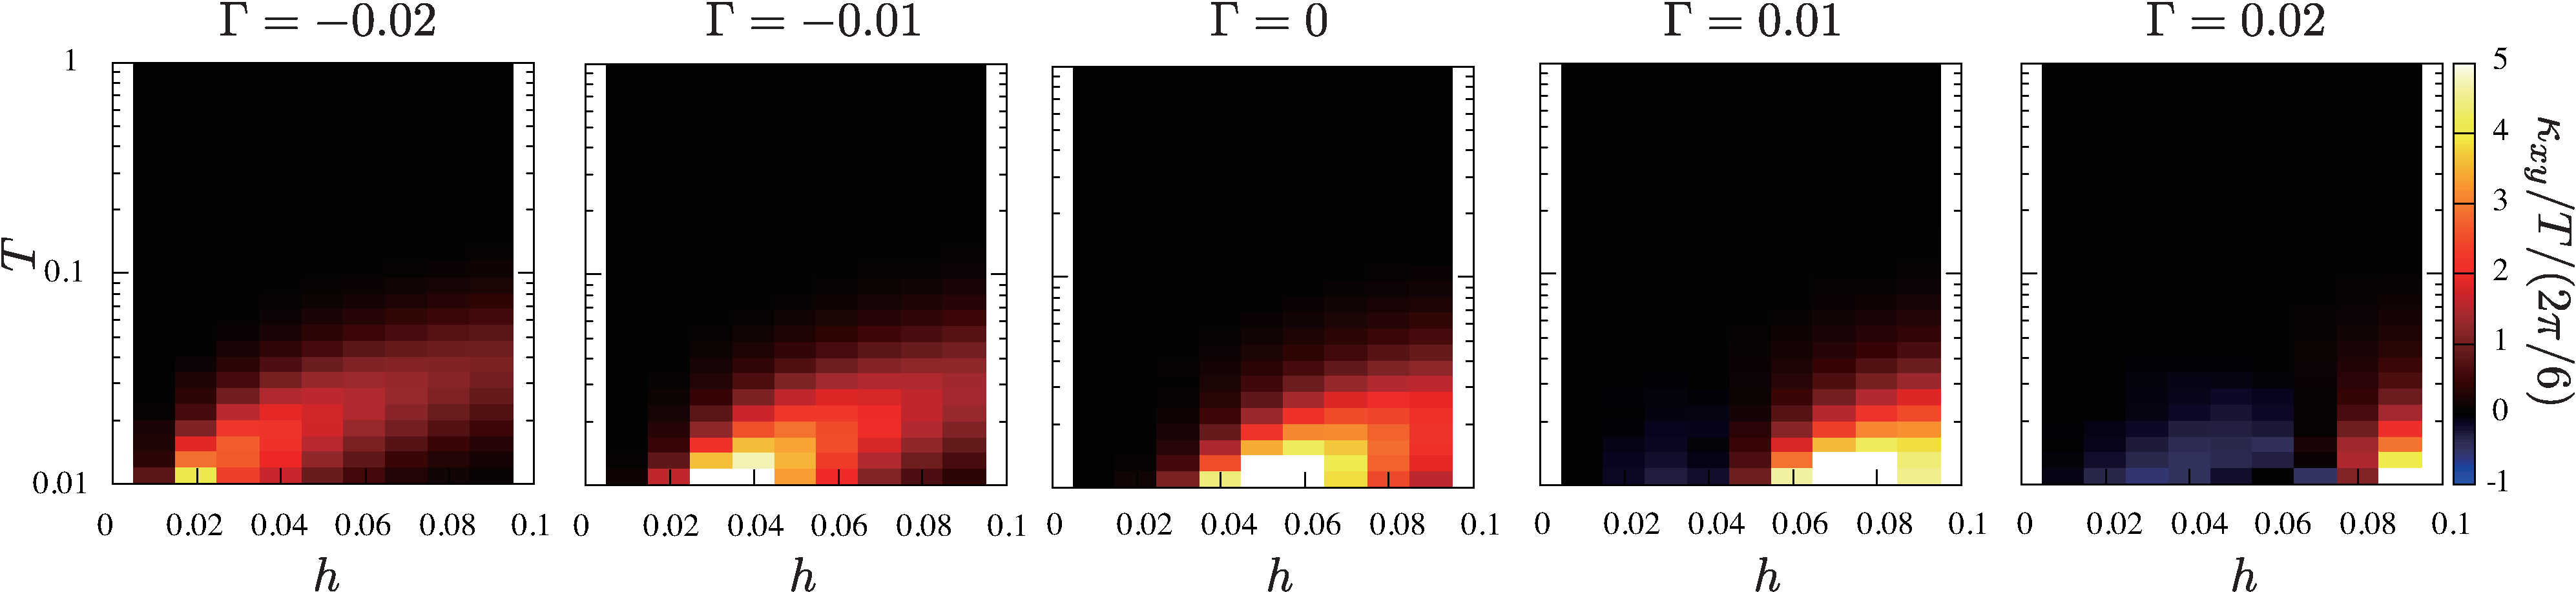
\includegraphics[width=\linewidth]{Figs/color_map_G_XC4.pdf}
%  \end{center}
%  \caption{Color maps of $\kappa_{xy}/T$ for ferromagnetic Kitaev model with $\Gamma = 0, \pm 0.01, \pm 0.02$ with various magnetic fields and temperatures. The lattice is \red{$(L, L') = (8, 4)$}.}
%  \label{fig:color_map_G_XC4}
%\end{figure*}

%\begin{figure*}
%  \begin{center}
%    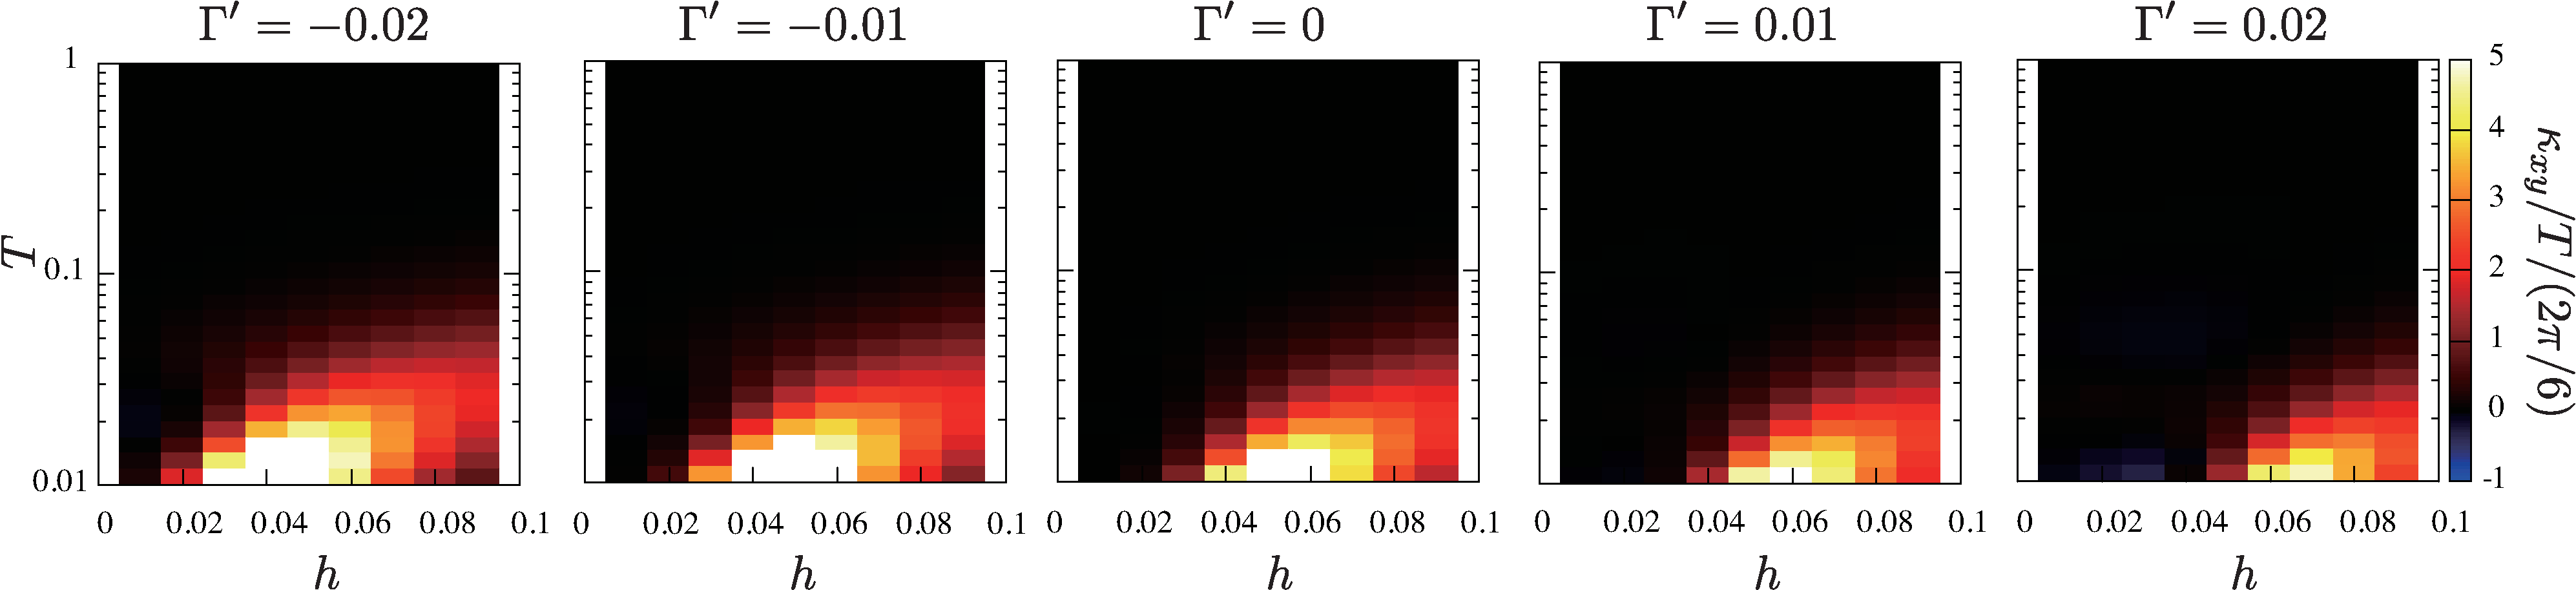
\includegraphics[width=\linewidth]{Figs/color_map_Gp_XC4.pdf}
%  \end{center}
%  \caption{Color maps of $\kappa_{xy}/T$ for ferromagnetic Kitaev model with $\Gamma' = 0, \pm 0.01, \pm 0.02$ with various magnetic fields and temperatures. The lattice is \red{$(L, L') = (8, 4)$}.}
%  \label{fig:color_map_Gp_XC4}
%\end{figure*}

\bibliography{Kitaev_kxy}
\end{document}
